\documentclass[11pt,a4paper]{scrartcl}

% ===================== PACKAGES =====================
\usepackage[british,UKenglish,USenglish,english,american]{babel}
\usepackage[tmargin=1in, bmargin=1in, lmargin=0.75in, rmargin=0.75in]{geometry}
\usepackage{tikz}
\usepackage{graphicx}
\usepackage{pgfplots}
\pgfplotsset{width=12cm, compat=1.9}
\usepackage{setspace}
\usepackage{chemmacros}
\usepackage{chemfig}
\usepackage{esint}
\usepackage{tabularray}
\usepackage{makeidx}
\usepackage{epstopdf}
\usepackage{amssymb}
\usepackage{mathrsfs}
\usepackage{bm}
\usepackage{amsmath}
\usepackage{enumitem}
\usepackage[english]{varioref}
\usepackage{lipsum}
\usepackage{fancyhdr}
\usepackage{float}
\usepackage{empheq}
\usepackage[framemethod=tikz]{mdframed}
\numberwithin{equation}{section}
\usepackage{eso-pic}
\usepackage{calc}
\usepackage{nccmath}
\usepackage{caption}
\usepackage{subcaption}
\usepackage{gensymb}
\usepackage{amsfonts, amsthm, epsfig, epstopdf, titling, url, array}
\usepackage{tabularx}
\usepackage{makecell}
\usepackage{booktabs}
\usepackage{array}
\usepackage{siunitx}
\sisetup{input-digits=0123456789\pi}
\usepackage[symbol]{footmisc}
\usepackage{xcolor}
\usepackage{multicol}
\usepackage{boondox-cal}
\usepackage{blindtext}
\usepackage{changepage}

% ===================== SI UNITS =====================
\DeclareSIUnit\atm{atm}

% ===================== PAGE STYLE =====================
\pagestyle{fancy}
\fancypagestyle{firstpage}{\rhead{}}
\fancyhead[L]{\slshape\nouppercase{\leftmark}}
\chead{}
\rhead{}
\lfoot{\textit{}}
\cfoot{-\ \thepage\ -}
\rfoot{\textit{}}
\renewcommand{\headrulewidth}{0.4pt}
\renewcommand{\footrulewidth}{0.4pt}

% ===================== MATH OPERATORS =====================
\DeclareMathOperator{\rank}{rank}
\DeclareMathOperator{\atantwo}{atan2}
\DeclareMathOperator{\spn}{span}

% ===================== COMMANDS =====================
\newcommand{\abs}[1]{\left|#1\right|}
\newcommand{\sign}{\text{sign}}
\newcommand{\centered}[1]{\begin{tabular}{@{}l@{}} #1 \end{tabular}}

% ===================== COLORS =====================
\definecolor{mycolor1}{rgb}{0.97, 0.97, 0.97}
\definecolor{mycolor2}{rgb}{0.97, 0.97, 0.97}
\definecolor{tableShade}{gray}{0.9}

% ===================== THEOREM ENVIRONMENTS =====================
\theoremstyle{it}
\newtheorem{defn}{Definition}[section]
\newtheorem{assumption}{Assumption}[section]
\newtheorem{thm}{Theorem}[section]
\newtheorem{lemma}{Lemma}[section]
\newtheorem{corollary}{Corollary}[section]
\theoremstyle{definition}
\newtheorem{example}{Example}[section]

% ===================== CUSTOM ENVIRONMENTS =====================
\newenvironment{myitemize_1}{
	\begin{itemize}[topsep=0pt]
		\setlength{\topsep}{2pt}
		\setlength{\itemsep}{2pt}
		\setlength{\parskip}{2pt}
		\setlength{\parsep}{2pt}
	}{\end{itemize}}

\newmdenv[
innerlinewidth=0.5pt,
roundcorner=4pt,
backgroundcolor=mycolor2,
linecolor=mycolor1,
innerleftmargin=6pt,
innerrightmargin=6pt,
innertopmargin=6pt,
innerbottommargin=6pt
]{mybox}

% ===================== TABLE COLUMN TYPES =====================
\newcolumntype{Y}{>{\hsize=2\hsize}X}
\newcolumntype{Z}{>{\centering\arraybackslash\hsize=0.857\hsize}X}

% ===================== SECTION DEPTH =====================
\setcounter{secnumdepth}{3}
\setcounter{tocdepth}{3}

\title{\textbf{ 
	\begin{LARGE}
		Single Phase Inverter:
	\end{LARGE} \\[12pt]
	\begin{LARGE}
		architecture, control, and simulation results.
	\end{LARGE}
	}
}
\author{\textbf{Davide Bagnara}}

\begin{document}
	\thispagestyle{firstpage}
	\begin{mybox}
		\maketitle
		\vspace{100mm}
	\end{mybox}
	\newpage
	\tableofcontents
	\listoffigures	
	\listoftables
	\newpage
	
%\chapter*{}	
%\begin{adjustwidth}{50pt}{50pt}
%		\textit{In the present document the design and model derivation of a CLL-Resonant DC/DC converter is reported. The document includes the control strategy and additional control loops for load harmonic compensation.}
%\end{adjustwidth}
\begin{onehalfspace}
\section{Introduction}
In this document a study for a single phase inverter is shown. 

The document starts with a description of the hardware layout following with a description of the control architecture.

\section{Architecture}

\subsection{Hardware Layout}
System architecture can be assumed as Figure~\ref{architecture_figure_2} shows. \\
\begin{figure}[H]
	\centering
	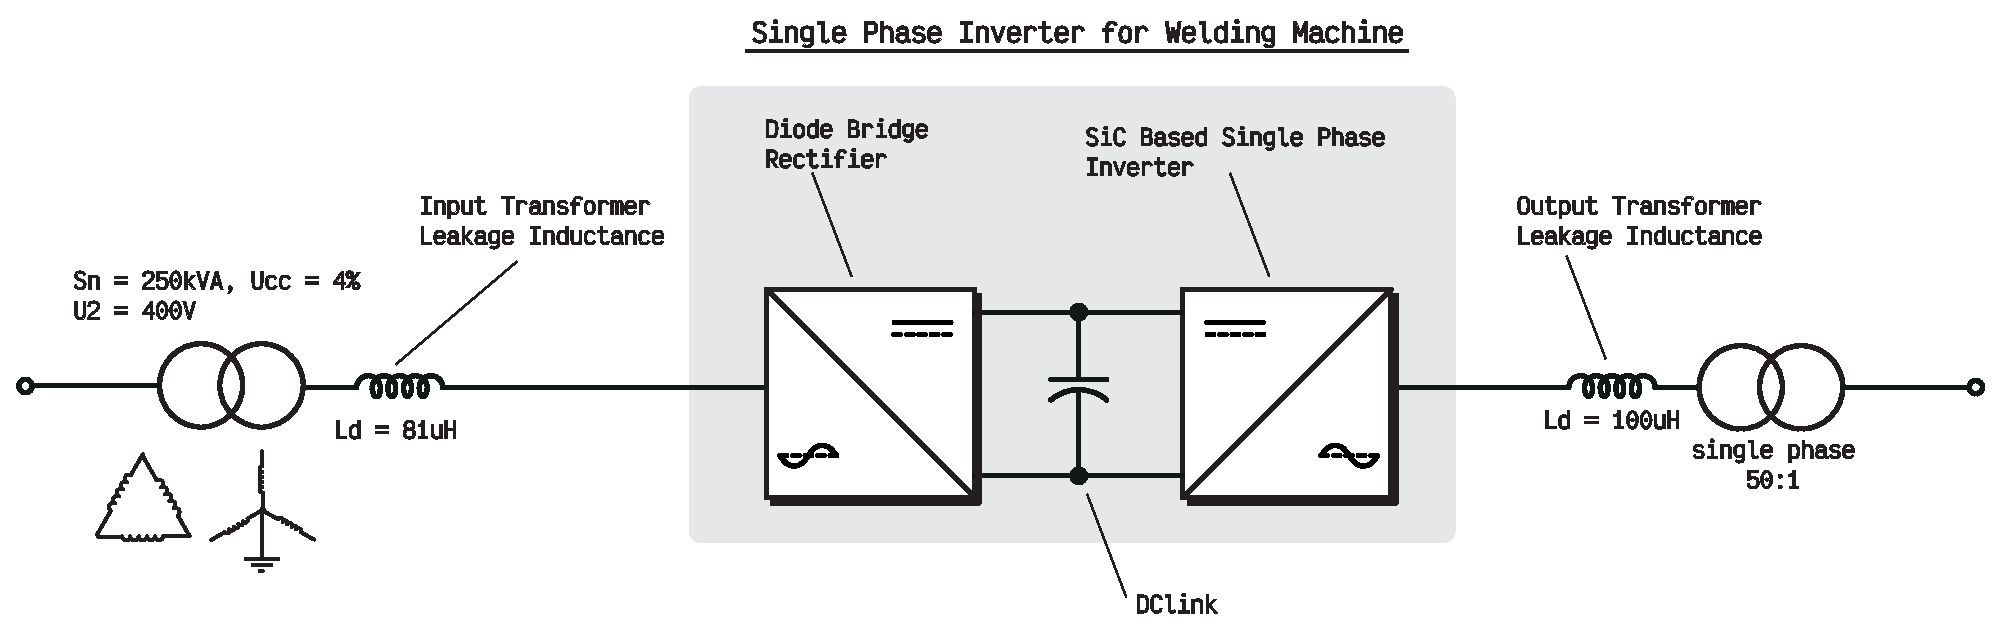
\includegraphics[width = 475pt, angle = 0, 
	keepaspectratio]{figures/arc/architecture_figure_2.eps}
	\captionsetup{width=0.5\textwidth, font=small}
	\caption{System layout composed by a grid with finite short circuit capability, a diode bridge rectifier, a dclink, a single phase inverter, and an output transformer with given leakage inductance.}
	\label{architecture_figure_2}
\end{figure}



\noindent\textbf{The system is composed by the following parts:}
\begin{itemize}
	\item[--] a grid power supply. It has been assumed that the system is connected to a 400V-250kVA three phase with a $U_{cc} = \SI{4}{\percent}$ which means an equivalent leakage inductance of $L_{d} = \SI{81}{\micro\henry}$;
	\item[--] a three phase diode bridge rectifier. The DClink voltage is generated by rectifying the 400V three phase voltage leading a nominal DClink voltage of $U_{dc}^{nom} = \SI{540}{\volt}$;
	\item[--] a DClink capacitor of value $C_{Fi} = \SI{5.6}{\milli\farad}$;
	\item[--] a SiC-MOSFET based full-bridge. The component selected is the module \textbf{SKM1700MB20R4S2I4} operating at the switching frequency of $f_{pwm} = \SI{20}{\kilo\hertz}$ per leg with an equivalent load switching frequency of $f_{load} = \SI{40}{\kilo\hertz}$;
	\item[--] the nominal inverter output current is $I_{out}^{nom} = \SI{600}{\ampere}$rms;
	\item[--] the load consists of an single phase transformer with a ratio factor of 50:1 (nominal secondary current of $I_2 = \SI{30}{\kilo\ampere}$);
\end{itemize}


\begin{figure}[H]
	\centering
	\begin{subfigure}{0.5\textwidth}
	\centering
	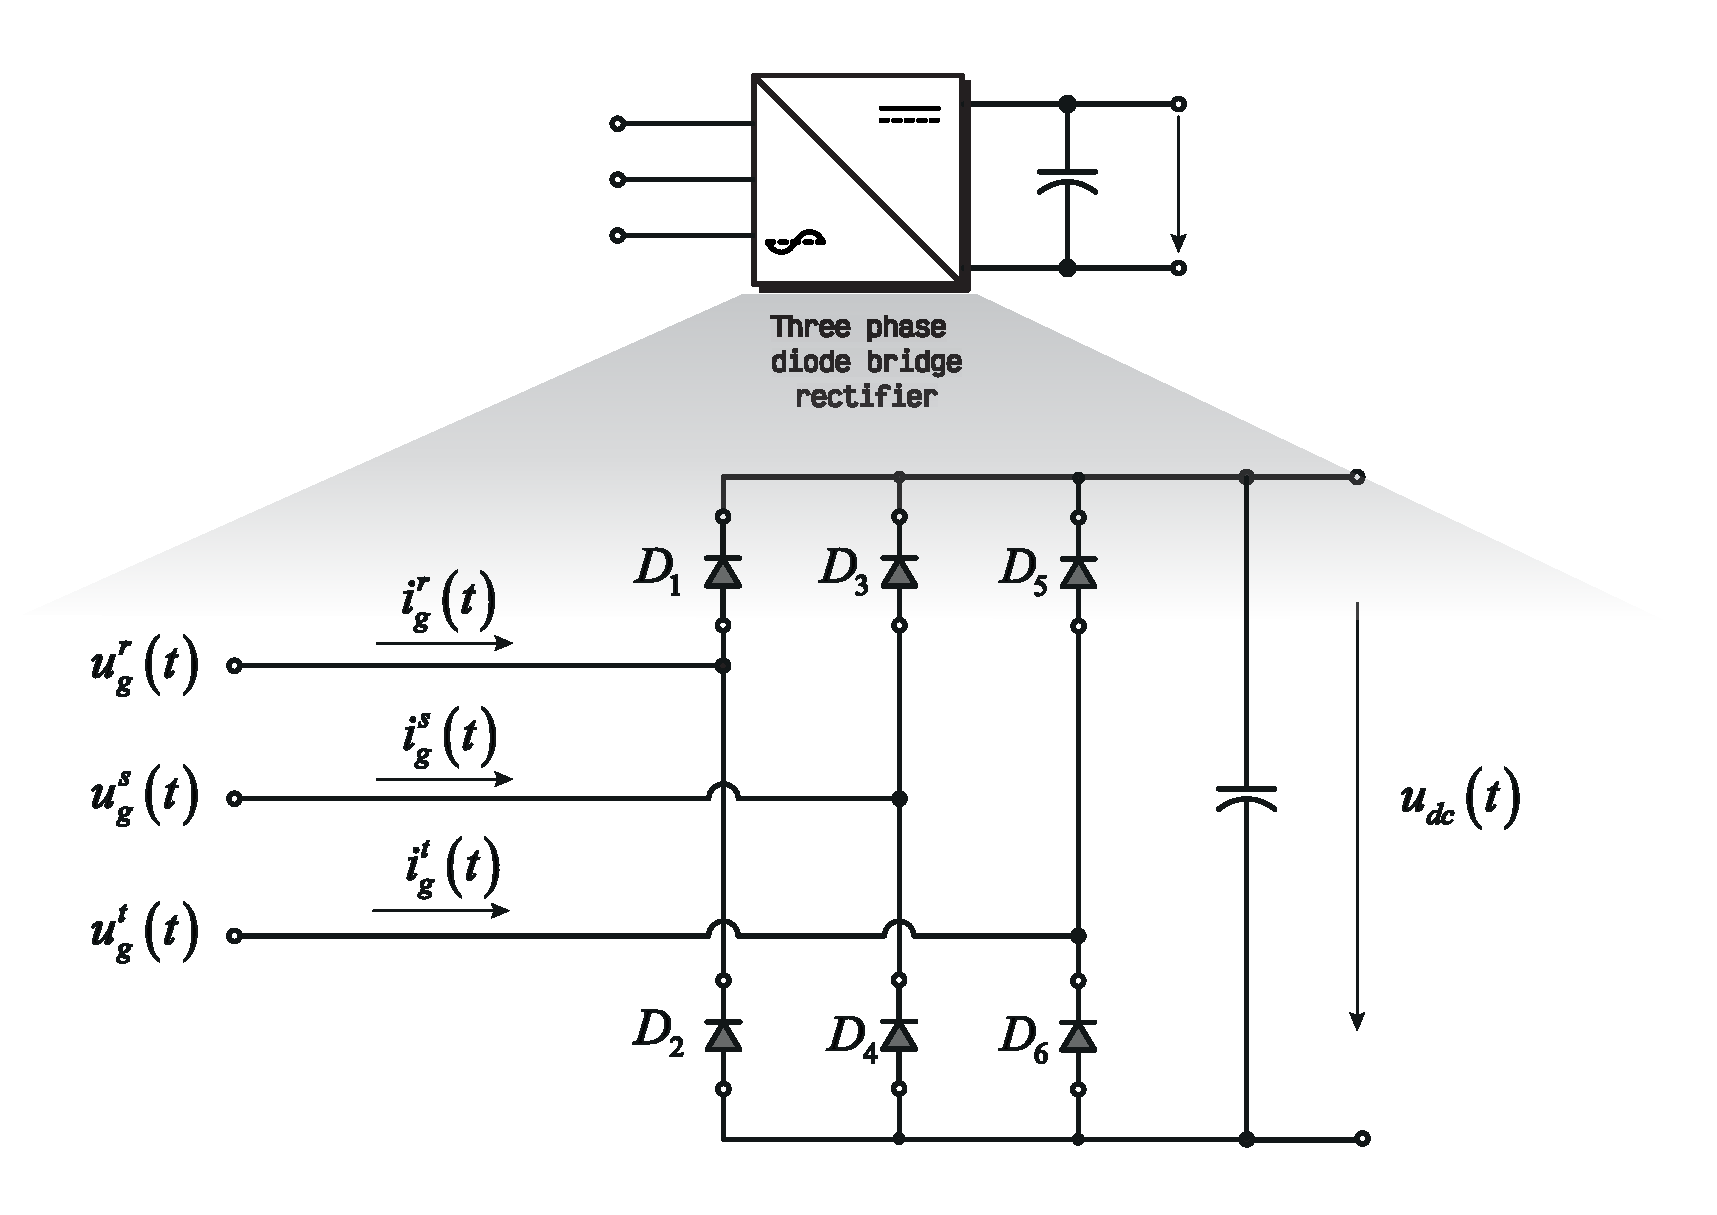
\includegraphics[width = 270pt, angle = 0, 
	keepaspectratio]{figures/arc/architecture_figure_3.eps}
	\captionsetup{width=0.5\textwidth, font=footnotesize}
	\caption{Input stage based on three phase diode rectifier and DClink capacitor.}
	\label{architecture_figure_3}
	\end{subfigure}%
	\begin{subfigure}{0.5\textwidth}
	\centering
	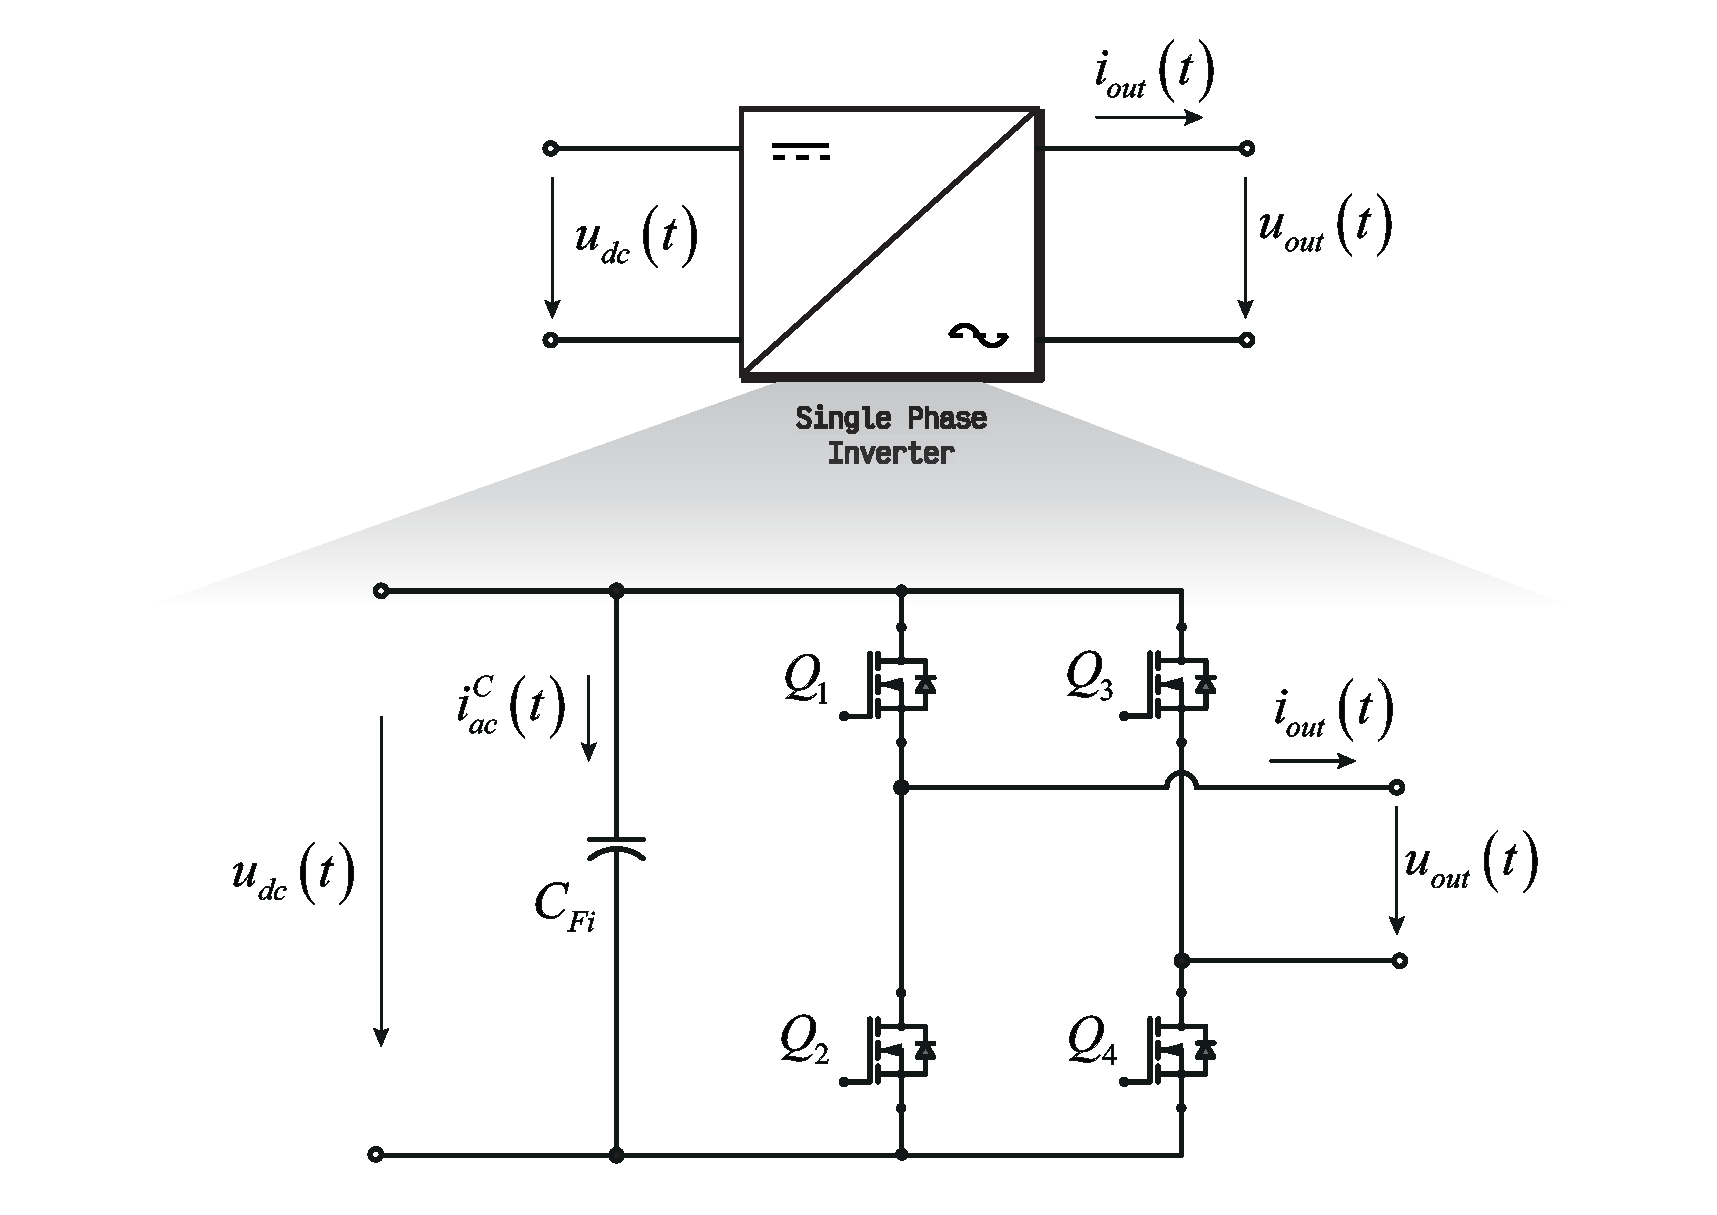
\includegraphics[width = 270pt, angle = 0, 
	keepaspectratio]{figures/arc/architecture_figure_1.eps}
	\captionsetup{width=0.5\textwidth, font=footnotesize}
	\caption{Single phase inverter based on SiC-MOSFET based full bridge.}
	\label{architecture_figure_1}
	\end{subfigure}
	\captionsetup{width=0.65\textwidth, font=small}	
	\caption{System architecture elements.}
	\label{}
\end{figure}


\section{Control Architectures}
As mentioned, the single phase inverter will operate in current control mode. The control strategy adopted is based on a virtual DQ control, as shown in Figure~\ref{single_phase_inverter_control_1}.

The current control is implemented using a virtual $DQ$ control (here $\xi\eta$ notation is used), where the $\eta$ component is created by a phase shift filter of the form

\begin{figure}[H]
	\centering
	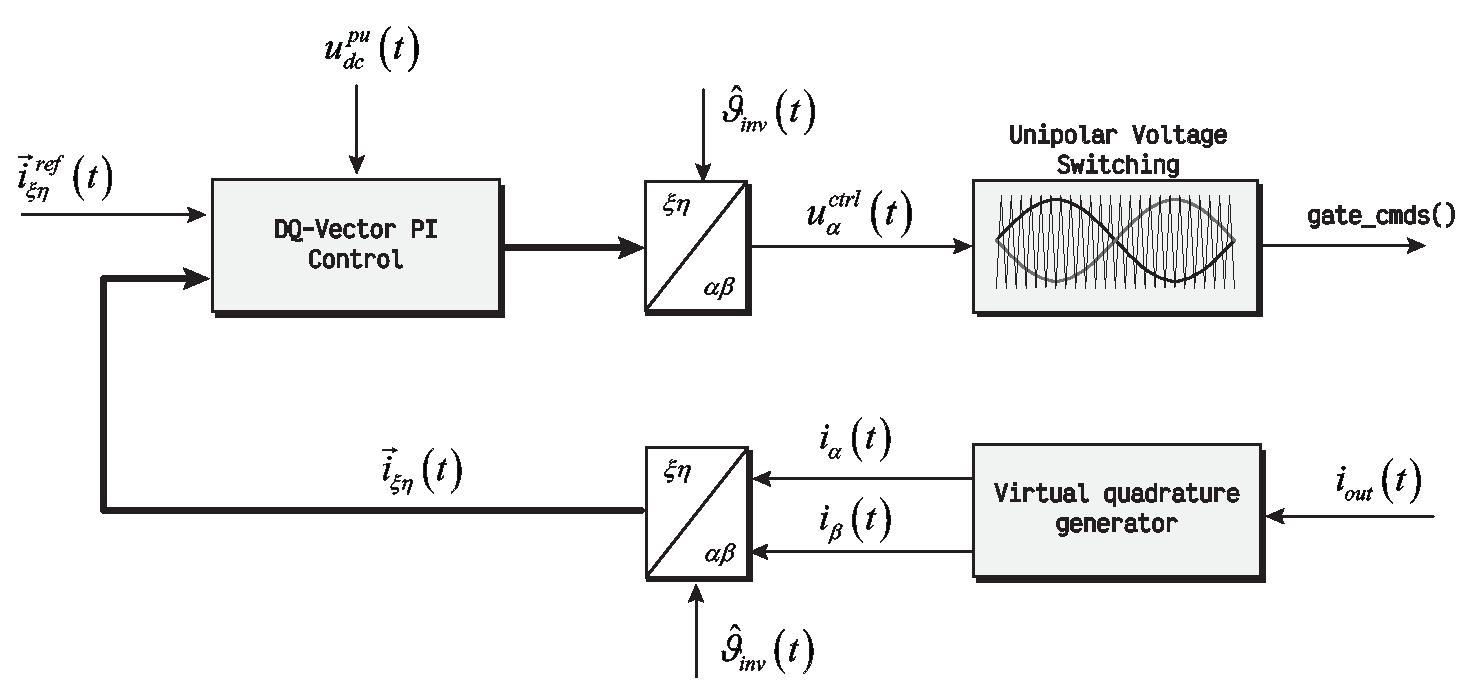
\includegraphics[width = 500pt, angle = 0, 
	keepaspectratio]{figures/ctrl/single_phase_inverter_control.eps}
	\captionsetup{width=0.5\textwidth, font=small}
	\caption{Current vector control layout of the single phase inverter. Virtual quadrature current is created by a phase shift filter.}
	\label{single_phase_inverter_control_1}
\end{figure}
\subsection{Nomenclature}	
Here, a list of used symbols:
\begin{itemize}
	\item[--] $i_{out}(t)$: inverter output current;
	\item[--] $u_{out}(t)$: inverter output voltage;	
	\item[--] $u_{dc}(t)$: DClink voltage;
	\item[--] $i_{ac}^{C}(t)$: DClink capacitor current;
	\item[--] $I_{ac}^{b}$: normalization AC current factor (end scale);
	\item[--] $U_{ac}^{b}$: normalization AC voltage factor (end scale);
	\item[--] $U_{dc}^{b}$: normalization DC voltage factor (end scale);
	\item[--] $i_{out}^{pu}(t) = i_{out}(t)/I_{ac}^{b}$ : normalized inverter output voltage;	
	\item[--] $i_\alpha = i_{out}^{pu}(t)$, load current respect to the stationary reference frame;
	\item[--] $i_\beta = i_\alpha(\omega t - \pi/2)$, phase shifted load current respect to the stationary reference frame, the phase shift is generated by an \textit{phase-shift-filter};
	\item[--] $\vartheta_{inv}(t)$ : inverter output phase internally generated when $f_{inv} \ne \SI{50}{\hertz}$ otherwise taken from grid phase lock loop (PLL);
	\item[--] $\omega = \dot{\vartheta}_{inv}(t)$
	\item[--] $u_{dc}^{pu} = u_{dc}(t)/U_{dc}^{b}$ : normalized DClink voltage;
	\item[--] $i_\xi(t) = i_\alpha(t)\cos(\omega t) + i_\beta(t)\sin(\omega t)$, load current component $\xi$ respect to the rotating reference frame;
	\item[--] $i_\eta(t) = -i_\alpha(t)\sin(\omega t) + i_\beta(t)\cos(\omega t)$, load current component $\eta$ respect to the rotating reference frame;
	\item[--] $u_\xi^{ctrl}(t)$, output current control of component $\xi$ respect to the rotating reference frame;
	\item[--] $u_\eta^{ctrl}(t)$, output current control of component $\eta$ respect to the rotating reference frame;
	\item[--] $u_\alpha^{ctrl}(t) = u_\xi^{ctrl}(t)\cos(\omega t) - u_\eta^{ctrl}(t)\sin(\omega t)$, output current control respect to the stationary reference frame;
\end{itemize}

\subsection{Normalization}
The per unit representation or \textit{normalization} plays a fundamental role for overall control tracking performance and shall be implemented as follows:
\begin{itemize}
	\item[--] Reference quantities
	\begin{itemize}
	\item[--] $i_{b} = I_{ac}^{b}$: normalization AC current factor (end scale);
	\item[--] $u_{b} = U_{ac}^{b}$: normalization AC voltage factor (end scale);
	\item[--] $\omega^{b} = 2\pi f = \frac{d}{dt}\vartheta_{inv}(t)$: normalization factor of the electrical pulsation;
	\end{itemize}
	\item[--] Per unit quantities
	\begin{itemize}
		\item[--] $R_{load}^{norm} = R_{load}/X^{b}$ : per unit representation of the load resistance;
		\item[--] $L_{load}^{norm} = L_{load}/L^{b}$ : per unit representation of the load inductance;
		\item[--] $\omega^{norm} = \omega/\omega^{b}$ : per unit of the electrical pulsation;		
		\item[--] $i^{norm} = i/i_{b}$ : per unit of $i$ current;
		\item[--] $u^{norm} = u/u_{b}$ : per unit of $u$ voltage;
		\item[--] $X^{b} = u_{b}/i_{b}$ : per unit of the linkage permanent magnet flux;
		\item[--] $L^{b} = X^{b}/\omega^{b}$ : per unit of the linkage permanent magnet flux.
	\end{itemize}	 
\end{itemize}

\subsection{Inner current control based on DQ-Vector PI}	


\begin{figure}[H]
	\centering
	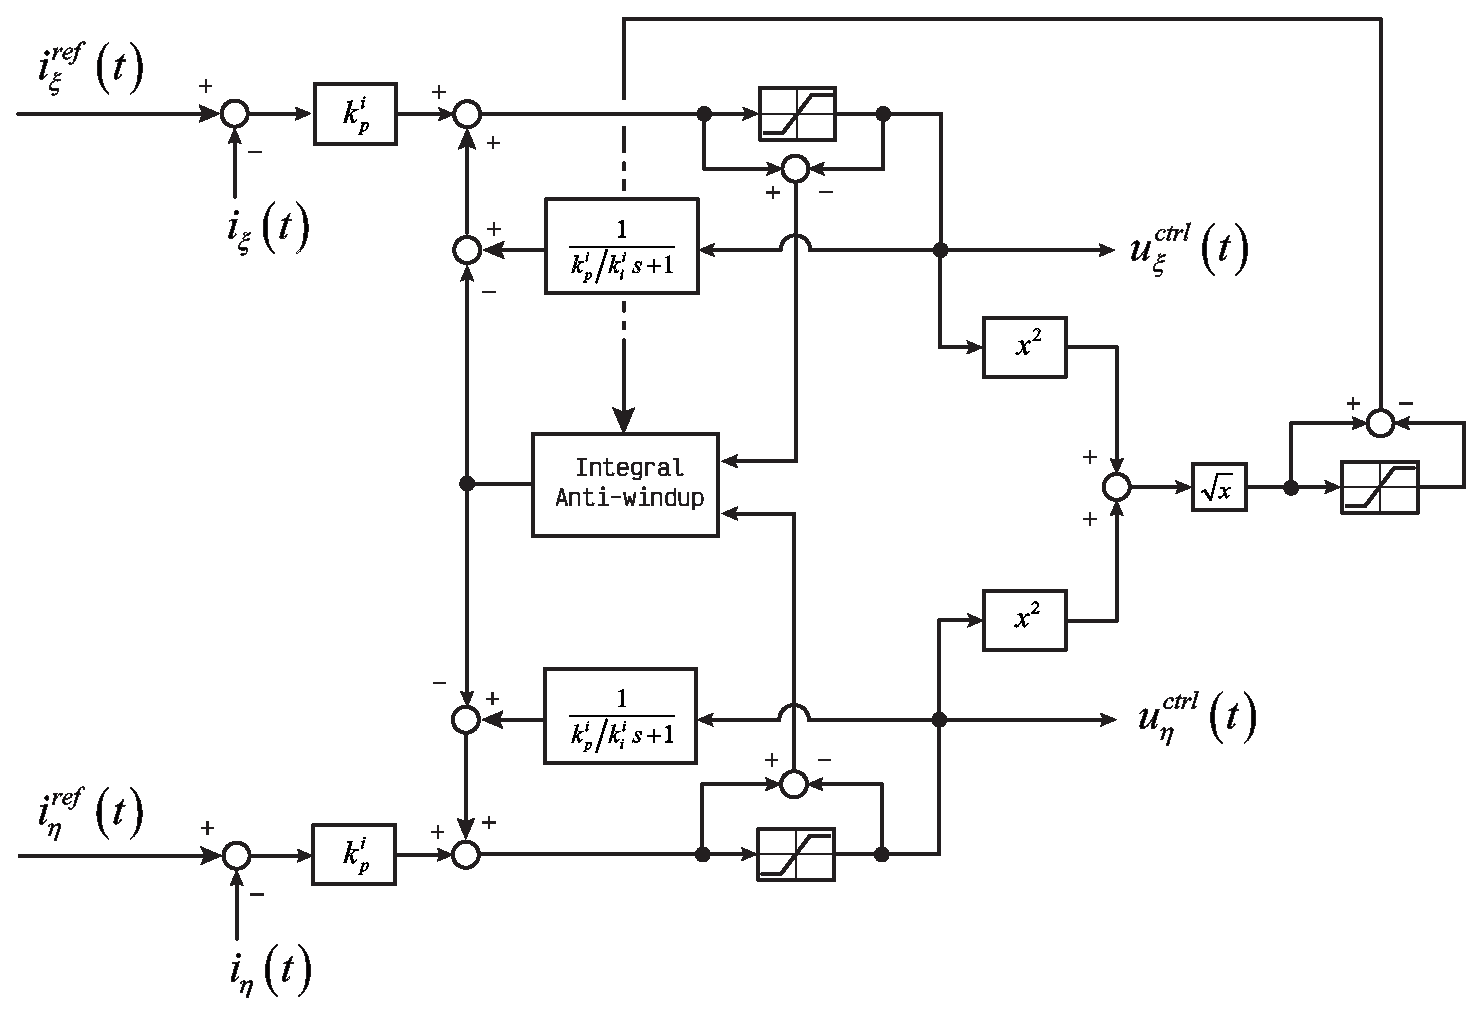
\includegraphics[width = 400pt, angle = 0, 
	keepaspectratio]{figures/ctrl/vector_pi_2.eps}
	\captionsetup{width=0.5\textwidth, font=small}
	\caption{Vector-PI control, where anti-windup is generated by three over-length conditions: on phase D, on phase Q, and on vector amplitude.}
	\label{vector_pi_2}
\end{figure}



\section{Simulation Results}

\subsection{Output frequency at 50Hz}

\begin{table}[H]
	%	\footnotesize
	\small
	\begin{center}	
		\begin{tblr}{p{0.75\linewidth}|p{0.25\linewidth}}
			\textbf{Quantity} & \textbf{value} \\
			\hline
			Load current reference				& $i_{out}^{ref} = \SI{600}{\ampere}$ rms \\	
			Load inductance	(at primary side)					& $L_{load} = \SI{400}{\micro\henry}$ \\	
			Load resistance (at primary side)						& $R_{load} = \SI{250}{\milli\ohm}$ \\	
			Load frequency 						& $f_{load} = \SI{50}{\hertz}$ \\
			Switching frequency (per leg) 		& $f_{sw} = \SI{10}{\kilo\hertz}$ \\
			DClink voltage 						& $v_{dc}=\SI{540}{\volt}$ \\
			External gate ON resistance 		& $R_g^{on}=\SI{0}{\ohm}$ \\			
			External gate OFF resistance 		& $R_g^{off}=\SI{0}{\ohm}$ \\
			Turn-On Switching Energy ($R_g^{on}=\SI{0.75}{\ohm}$, $T_j=\SI{150}{\celsius}$, $u_{dc}=\SI{1300}{\volt}$, $i_{d}=\SI{1000}{\ampere}$) 			& $E_{on}=\SI{1.56}{\milli\joule}$ \\
			Turn-Off Switching Energy ($R_g^{off}=\SI{1.3}{\ohm}$, $T_j=\SI{150}{\celsius}$, $u_{dc}=\SI{1300}{\volt}$, $i_{d}=\SI{1000}{\ampere}$) 			& $E_{off}=\SI{0.84}{\milli\joule}$ \\
			Reserve Recovery Energy ($T_j=\SI{150}{\celsius}$, $u_{dc}=\SI{1300}{\volt}$, $i_{d}=\SI{1000}{\ampere}$) & $E_{rr}=\SI{0.075}{\milli\joule}$ \\
			MOSFET Thermal Resistance, Junction to Heatsink (per MOSFET) 	& $R_{jh}=\SI{25}{\celsius\per\kilo\watt}$ \\
			Thermal Interface Material (per MOSFET) 						& $R_{TIM}=\SI{5}{\celsius\per\kilo\watt}$ \\
			MOSFET Thermal Resistance, Heatsink to Ambient (per MOSFET) 	& $R_{ha}=\SI{7.5}{\celsius\per\kilo\watt}$ \\
			\hline
		\end{tblr}
	\end{center}
	\captionsetup{width=.5\textwidth, font=small}
	\caption{List of conditions for the electro-thermal simulation at $f_{load} = \SI{50}{\hertz}$.}
	\label{}
\end{table}	

\begin{table}[H]
	%	\footnotesize
	\small
	\begin{center}	
		\begin{tblr}{p{0.75\linewidth}|p{0.25\linewidth}}
			\textbf{Quantity} & \textbf{value} \\
			\hline
			Load current							& $i_{out} = \SI{600}{\ampere}$rms \\	
			Load voltage							& $u_{out} = \SI{238}{\volt}$ rms \\	
			Grid input active power					& $P_{g} = \SI{93}{\kilo\watt}$ \\				
			DClink capaciror current				& $i_{ac}^C = \SI{343}{\ampere}$rms \\	
			MOSFET Q1 rms current					& $i_{Q1} = \SI{424}{\ampere}$rms \\	
			MOSFET Q1 maximum voltage				& $u_{Q1}^{max} = \SI{620}{\volt}$ \\	
			MOSFET Q1 power losses					& $P_{Q1} = \SI{432}{\watt}$ \\	
			Module power losses						& $P_{m} = \SI{864}{\watt}$ \\
			Inverter power losses					& $P_{H} = \SI{1728}{\watt}$ \\
			MOSFET maximum J-H delta temperature	& $T_{jh}^{Q1} = \SI{90}{\celsius}$ \\	
			Diode rectifier rms current 			& $i_{dr} = \SI{400}{\ampere}$rms \\	
			\hline
		\end{tblr}
	\end{center}
	\captionsetup{width=.5\textwidth, font=small}
	\caption{List of data results for the electro-thermal simulation at $f_{load} = \SI{50}{\hertz}$.}
	\label{}
\end{table}	


\begin{figure}[H]
	\centering
	\begin{subfigure}{0.5\textwidth}
		\centering
		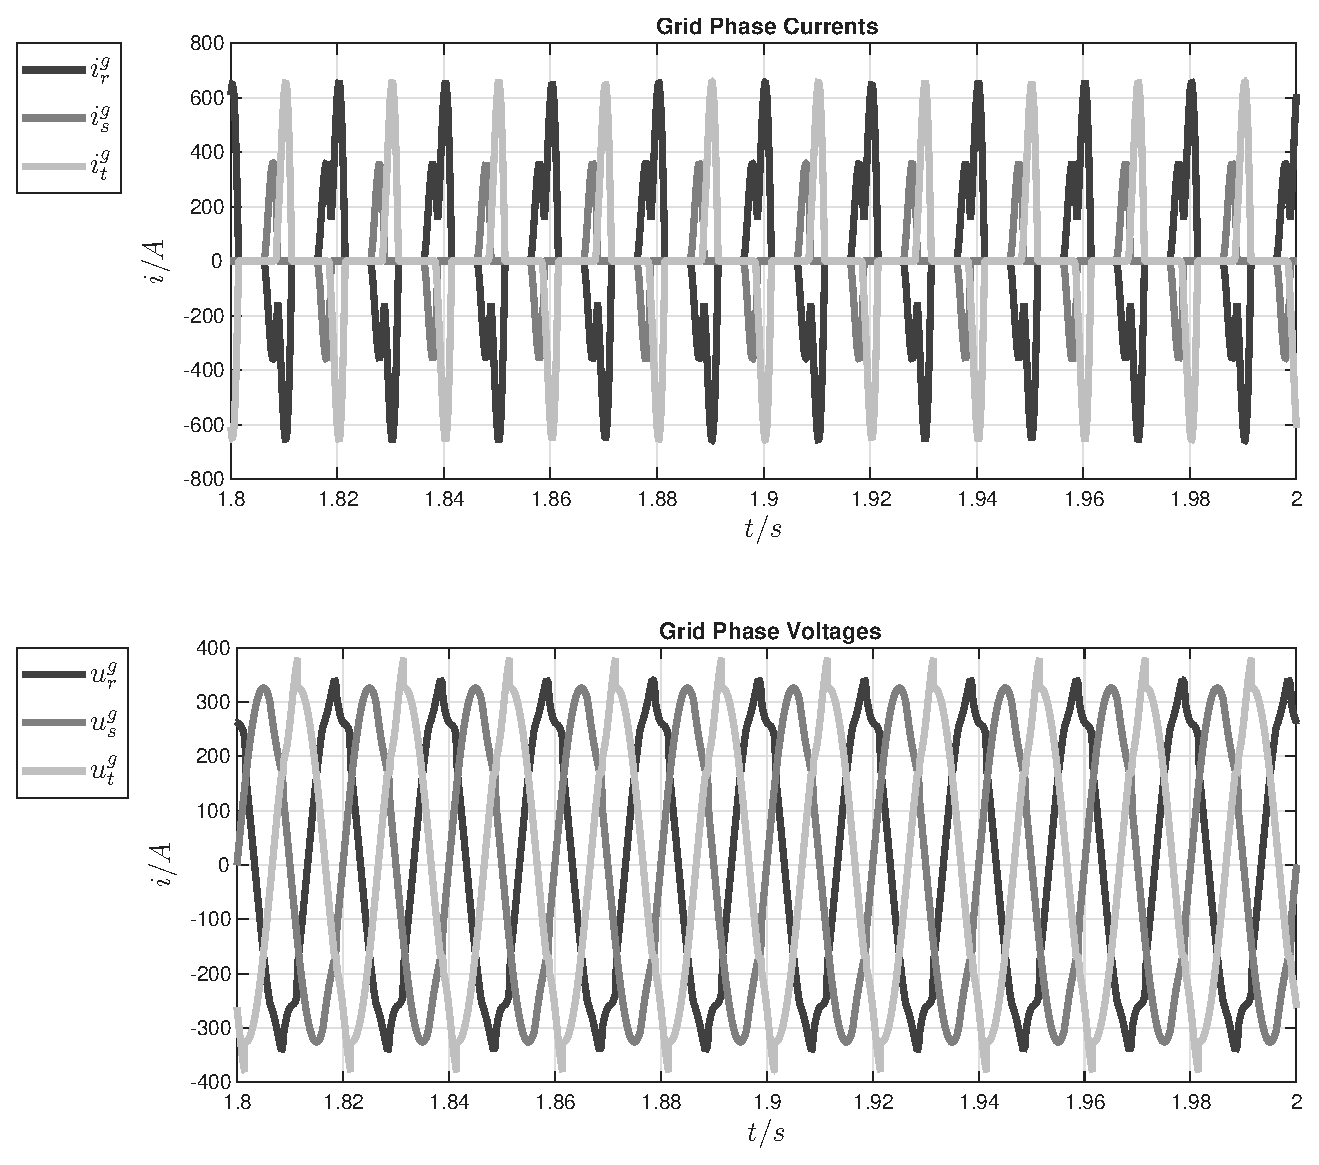
\includegraphics[width =225pt, angle = 0, 
		keepaspectratio]{figures/sim_results_50Hz_10kHz_1/grid_quantities.eps}
		\captionsetup{width=0.75\textwidth, font=footnotesize}	
		\caption{Grid currents (top), and grid voltages (bottom), supposing $S_{nom} = \SI{250}{\kilo\volt\ampere}$ and $U_{cc} = \SI{4}{\percent}$.}
		\label{grid_quantities}
	\end{subfigure}%
	\begin{subfigure}{0.5\textwidth}
		\centering
		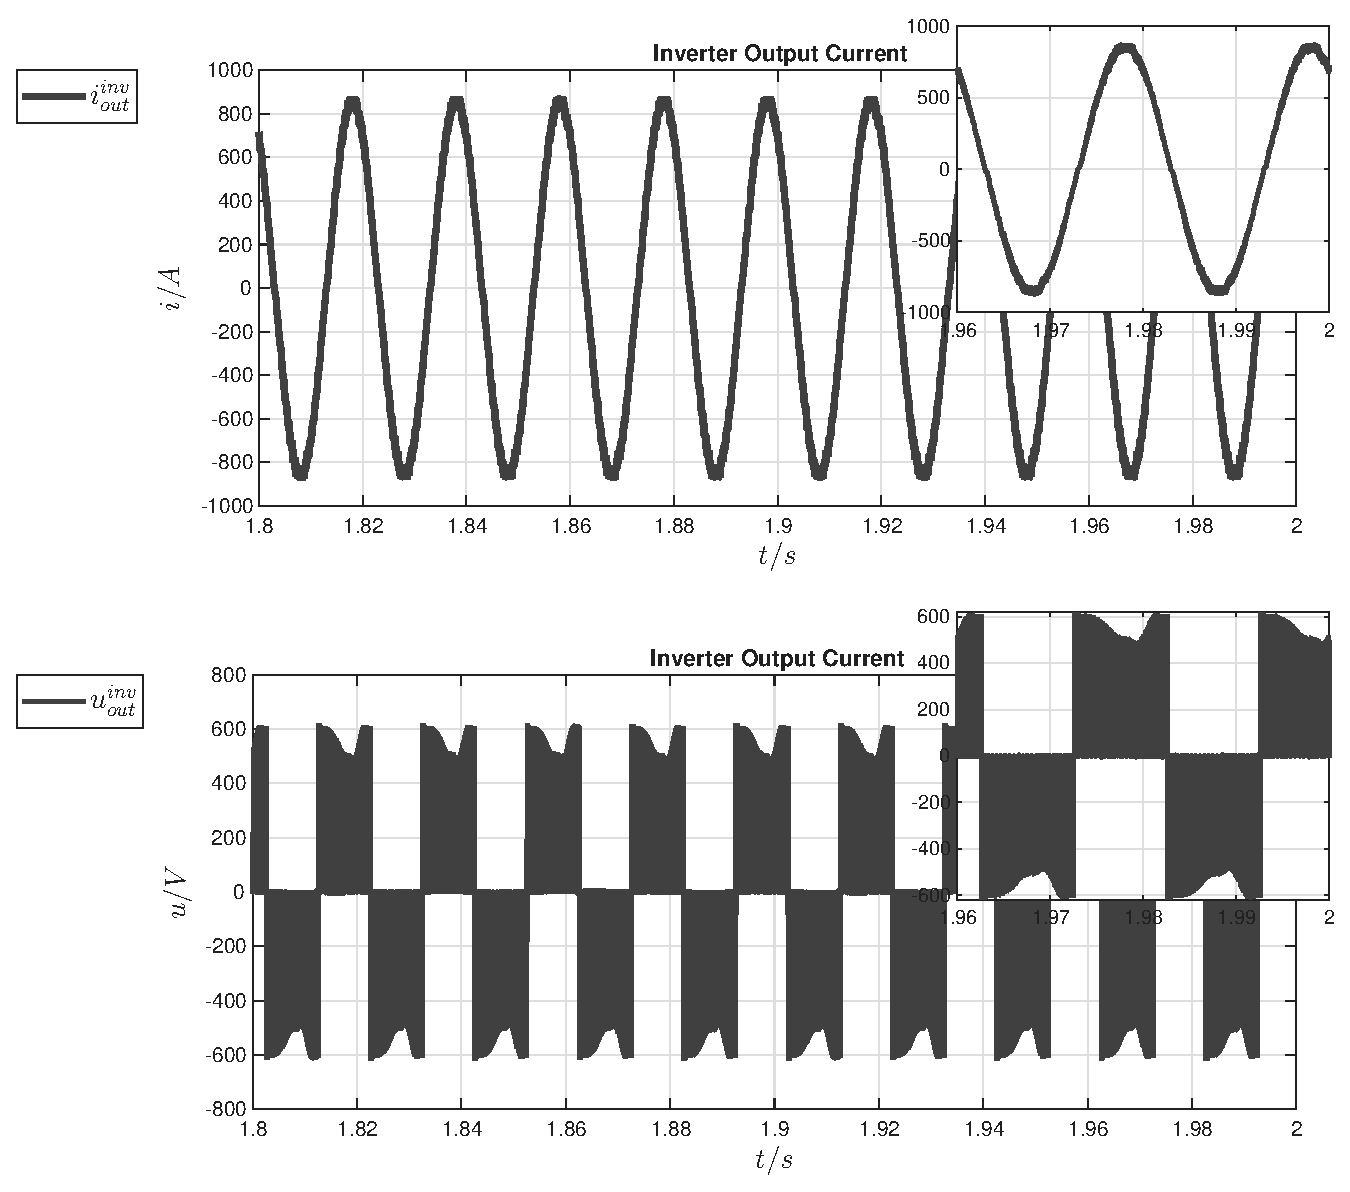
\includegraphics[width =225pt, angle = 0, 
		keepaspectratio]{figures/sim_results_50Hz_10kHz_1/inverter_output_current.eps}
		\captionsetup{width=0.75\textwidth, font=footnotesize}	
		\caption{Inverter output current (top), and inverter output voltage (bottom), supposing $f_{pwm} = \SI{10}{\kilo\hertz}$ per leg.}
		\label{inverter_output_current}
	\end{subfigure}
	\captionsetup{width=0.65\textwidth, font=small}	
	\caption{Grid and inverter output quantities.}
	\label{}
\end{figure}

\begin{figure}[H]
	\centering
	\begin{subfigure}{0.5\textwidth}
		\centering
		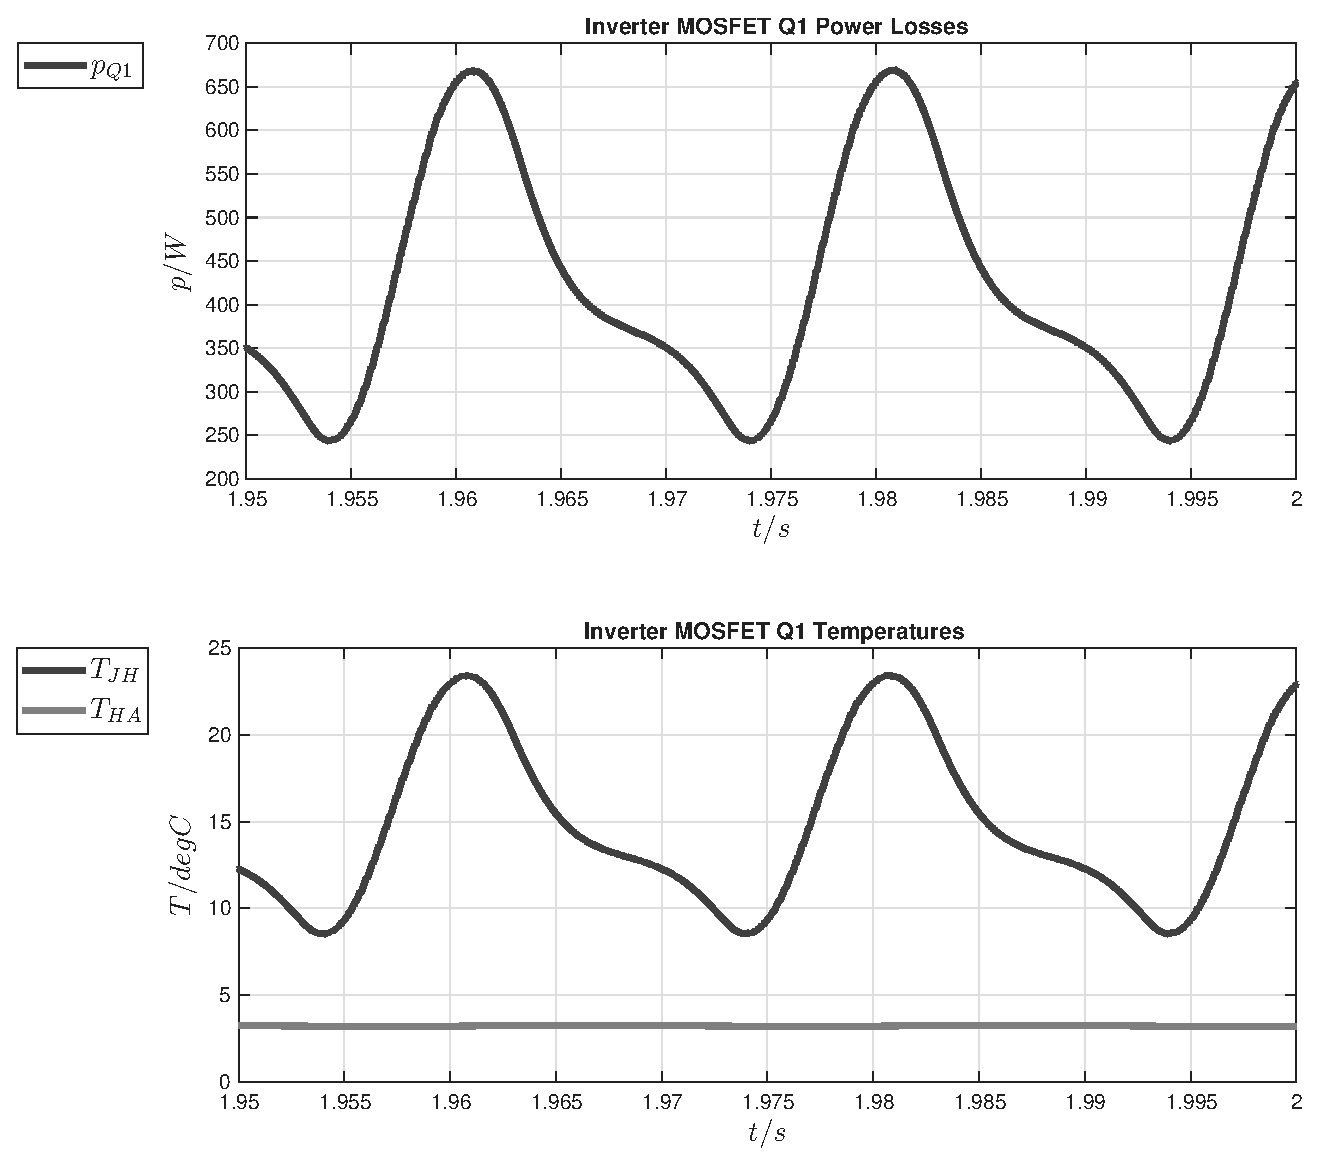
\includegraphics[width =225pt, angle = 0, 
		keepaspectratio]{figures/sim_results_50Hz_10kHz_1/inverter_Q1_power_losses.eps}
		\captionsetup{width=0.65\textwidth, font=footnotesize}	
		\caption{Inverter MOSFET Q1 power loss (top), and junction-case temperature (bottom).}
		\label{inverter_Q1_power_losses}
	\end{subfigure}%
	\begin{subfigure}{0.5\textwidth}
		\centering
		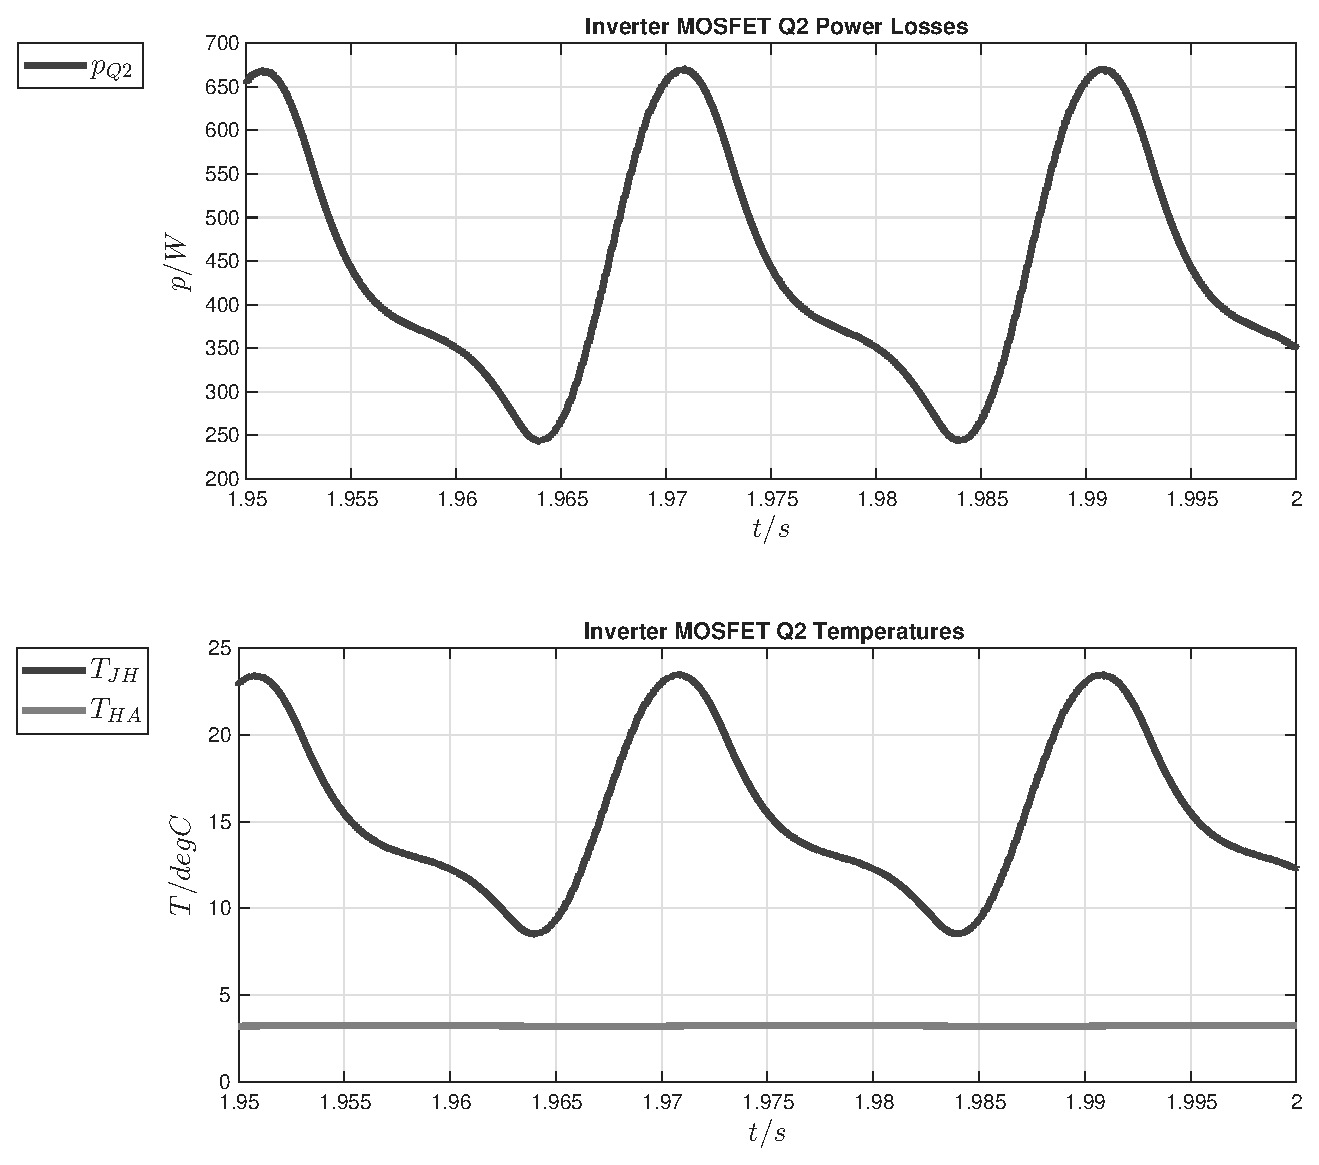
\includegraphics[width =225pt, angle = 0, 
		keepaspectratio]{figures/sim_results_50Hz_10kHz_1/inverter_Q2_power_losses.eps}
		\captionsetup{width=0.75\textwidth, font=footnotesize}	
		\caption{Inverter MOSFET Q2 power loss (top), and junction-case temperature (bottom).}
		\label{inverter_Q2_power_losses}
	\end{subfigure}
	\captionsetup{width=0.65\textwidth, font=small}	
	\caption{Inverter MOSFETs thermal performance.}
	\label{}
\end{figure}

\begin{figure}[H]
	\centering
	\begin{subfigure}{0.5\textwidth}
		\centering
		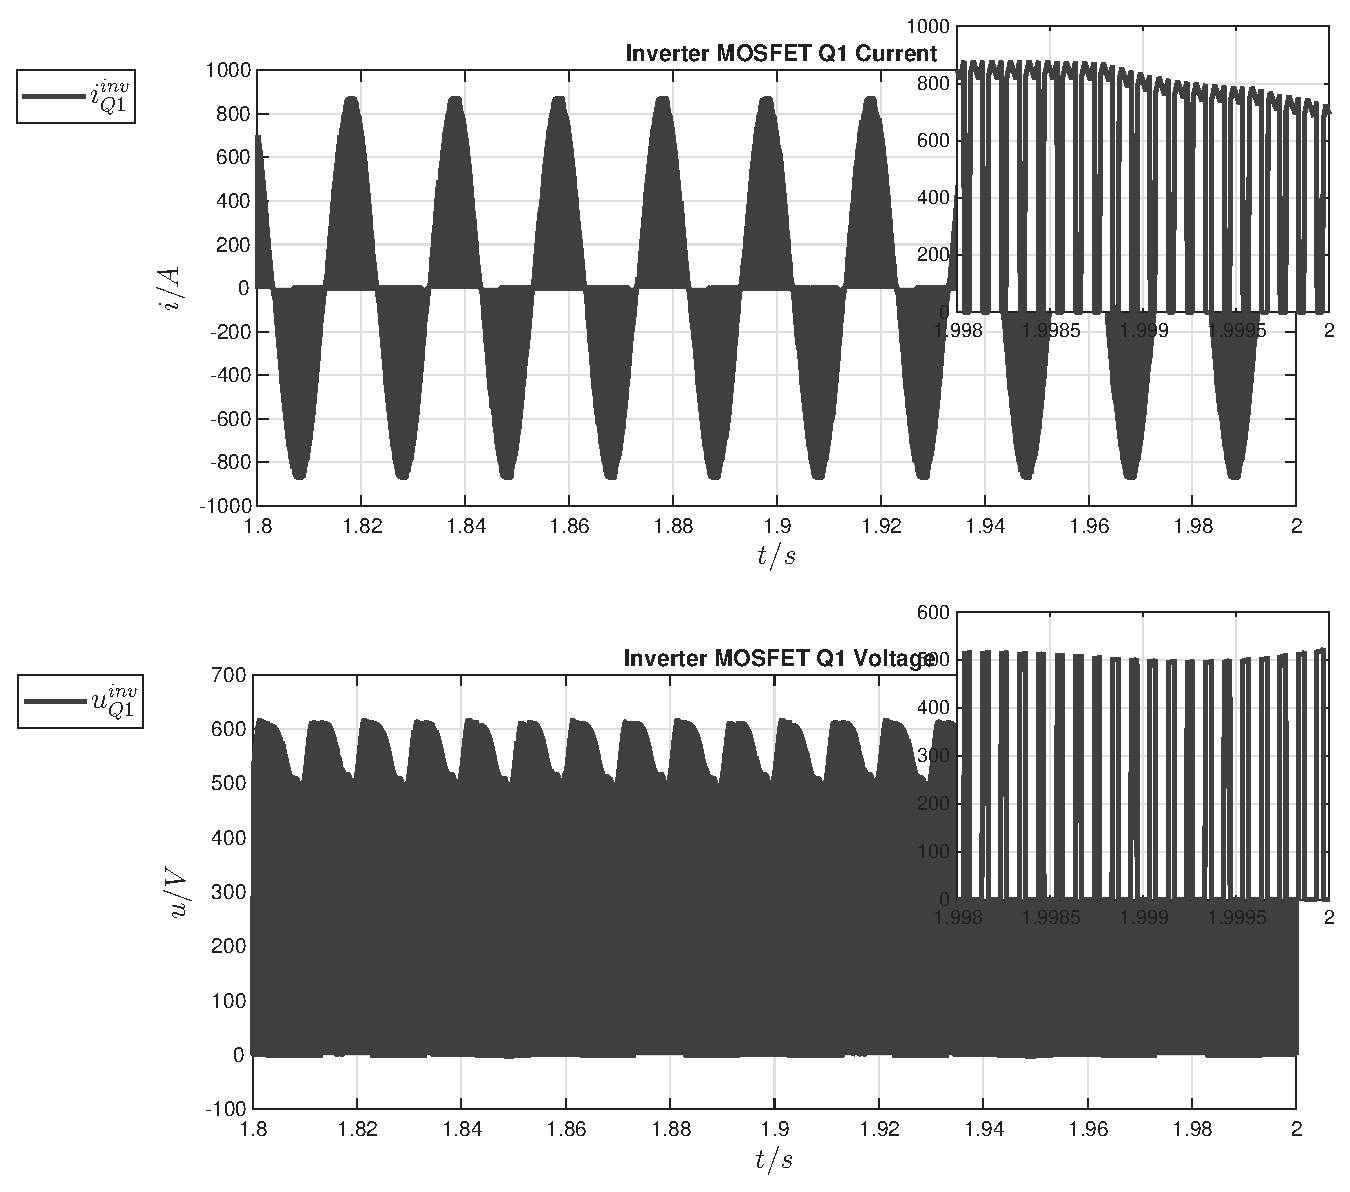
\includegraphics[width =225pt, angle = 0, 
		keepaspectratio]{figures/sim_results_50Hz_10kHz_1/inverter_mosfet_Q1_iu.eps}
		\captionsetup{width=0.65\textwidth, font=footnotesize}	
		\caption{Inverter MOSFET Q1 current (top), and voltage (bottom).}
		\label{inverter_mosfet_Q1_iu}
	\end{subfigure}%
	\begin{subfigure}{0.5\textwidth}
		\centering
		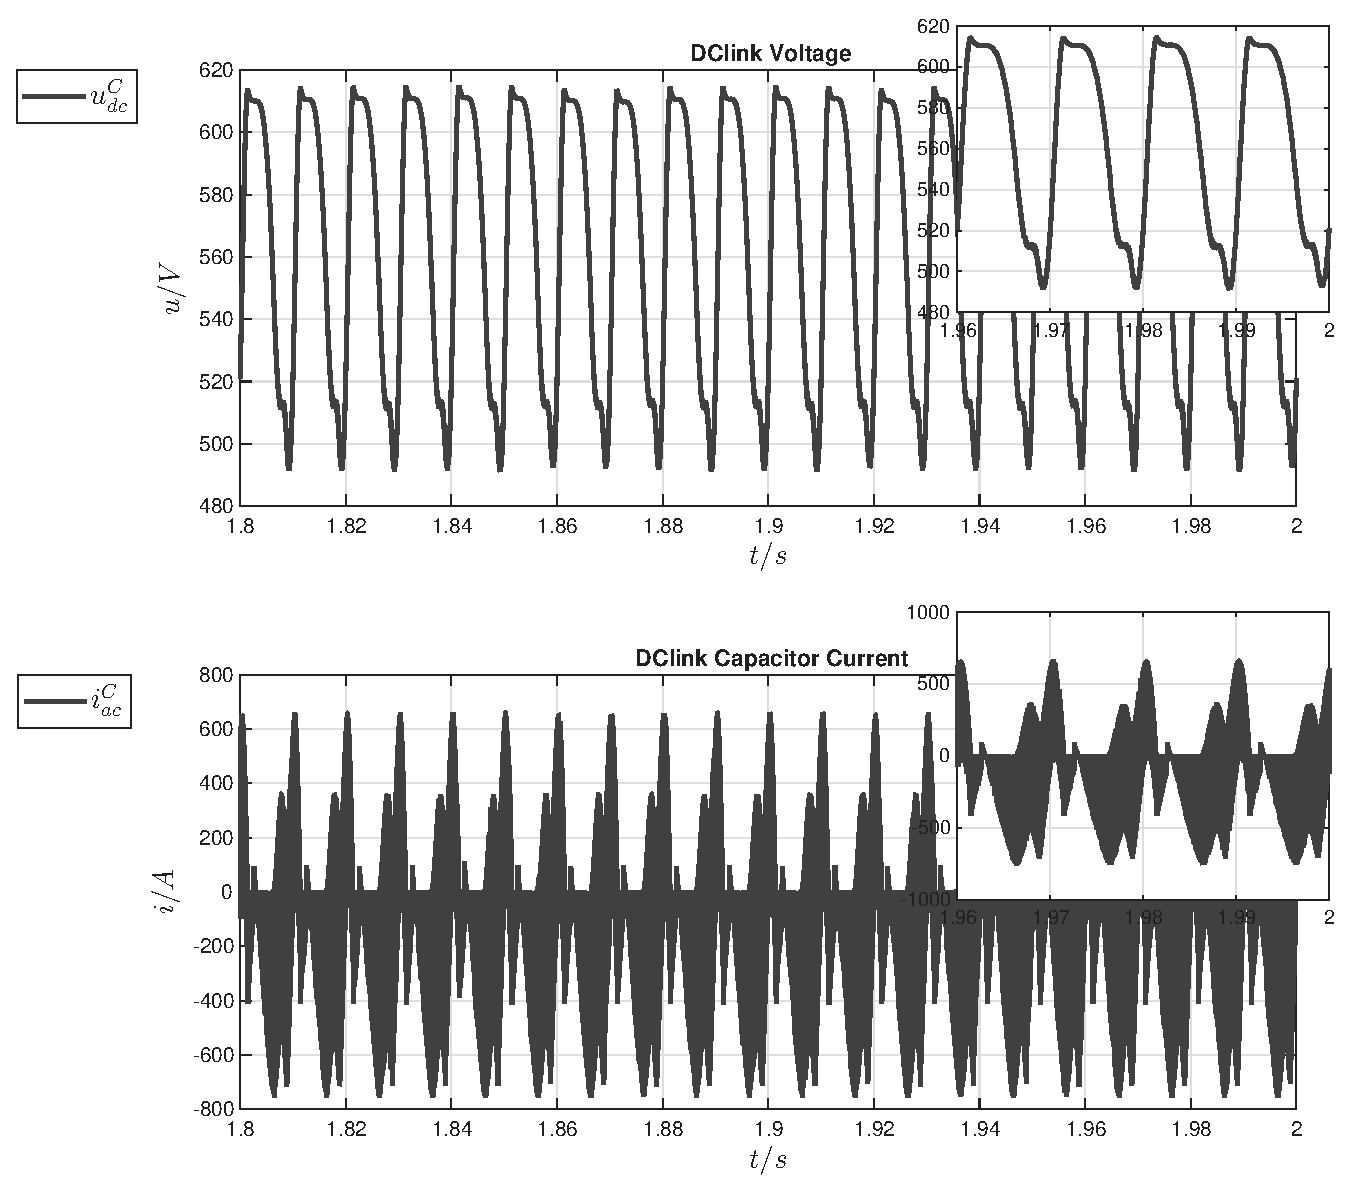
\includegraphics[width =225pt, angle = 0, 
		keepaspectratio]{figures/sim_results_50Hz_10kHz_1/dclink_ui.eps}
		\captionsetup{width=0.75\textwidth, font=footnotesize}	
		\caption{DClink voltage (top), and dclink capcitor current (bottom).}
		\label{dclink_ui}
	\end{subfigure}
	\captionsetup{width=0.65\textwidth, font=small}	
	\caption{Inverter MOSFETs, and DClink quantities.}
	\label{}
\end{figure}

\begin{figure}[H]
	\centering
	\begin{subfigure}{0.5\textwidth}
		\centering
		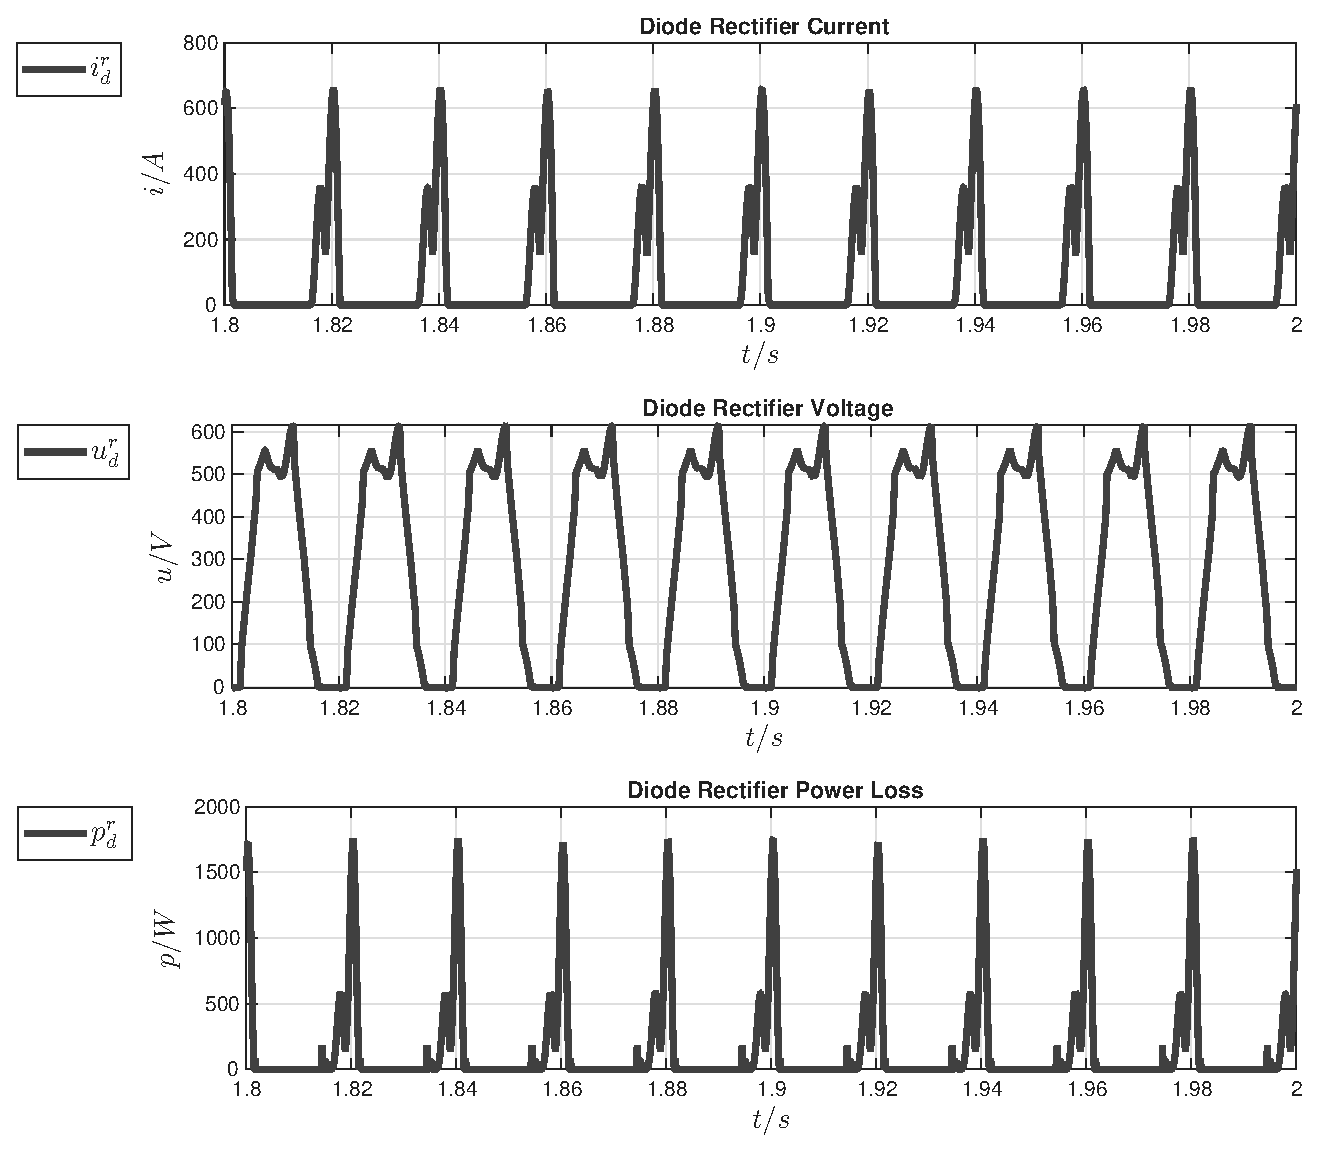
\includegraphics[width =225pt, angle = 0, 
		keepaspectratio]{figures/sim_results_50Hz_10kHz_1/diode_rectifier.eps}
		\captionsetup{width=0.65\textwidth, font=footnotesize}	
		\caption{Diode D1 rectifier current (top), voltage (center), and power loss (bottom).}
		\label{diode_rectifier}
	\end{subfigure}%
	\begin{subfigure}{0.5\textwidth}
		\centering
		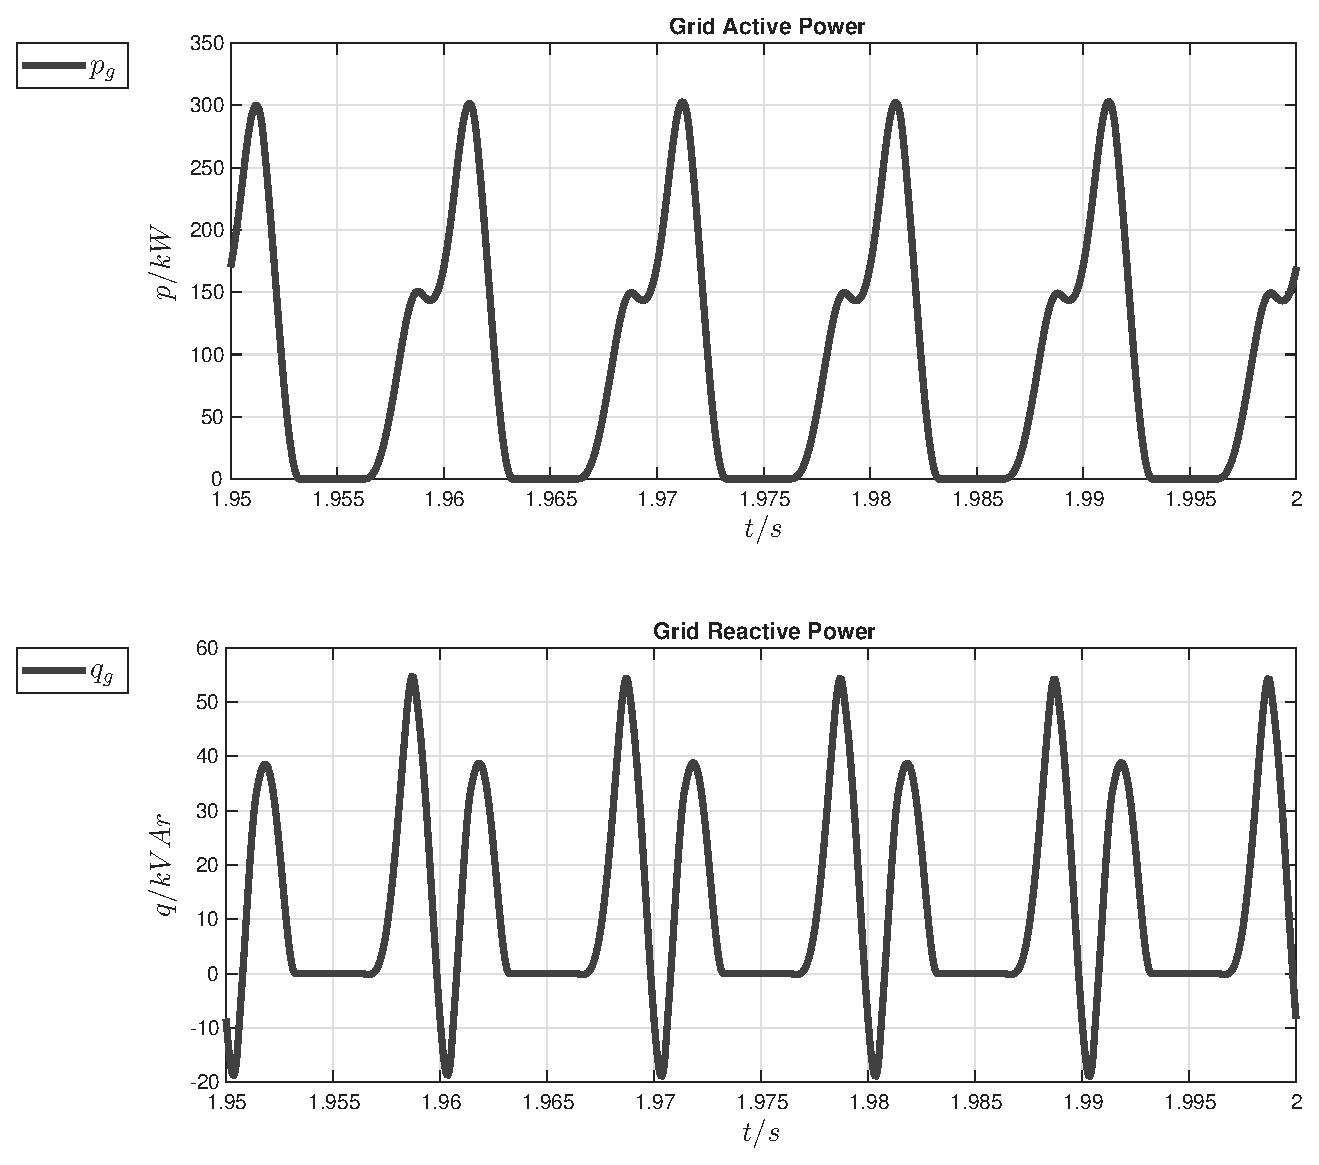
\includegraphics[width =225pt, angle = 0, 
		keepaspectratio]{figures/sim_results_50Hz_10kHz_1/grid_power.eps}
		\captionsetup{width=0.75\textwidth, font=footnotesize}	
		\caption{Grid active power (top), and grid reactive power (bottom) - measure implemented according to IEC.}
		\label{grid_power}
	\end{subfigure}
	\captionsetup{width=0.65\textwidth, font=small}	
	\caption{Rectifier diode quantities and grid power analysis.}
	\label{}
\end{figure}

\begin{figure}[H]
	\centering
	\begin{subfigure}{0.5\textwidth}
		\centering
		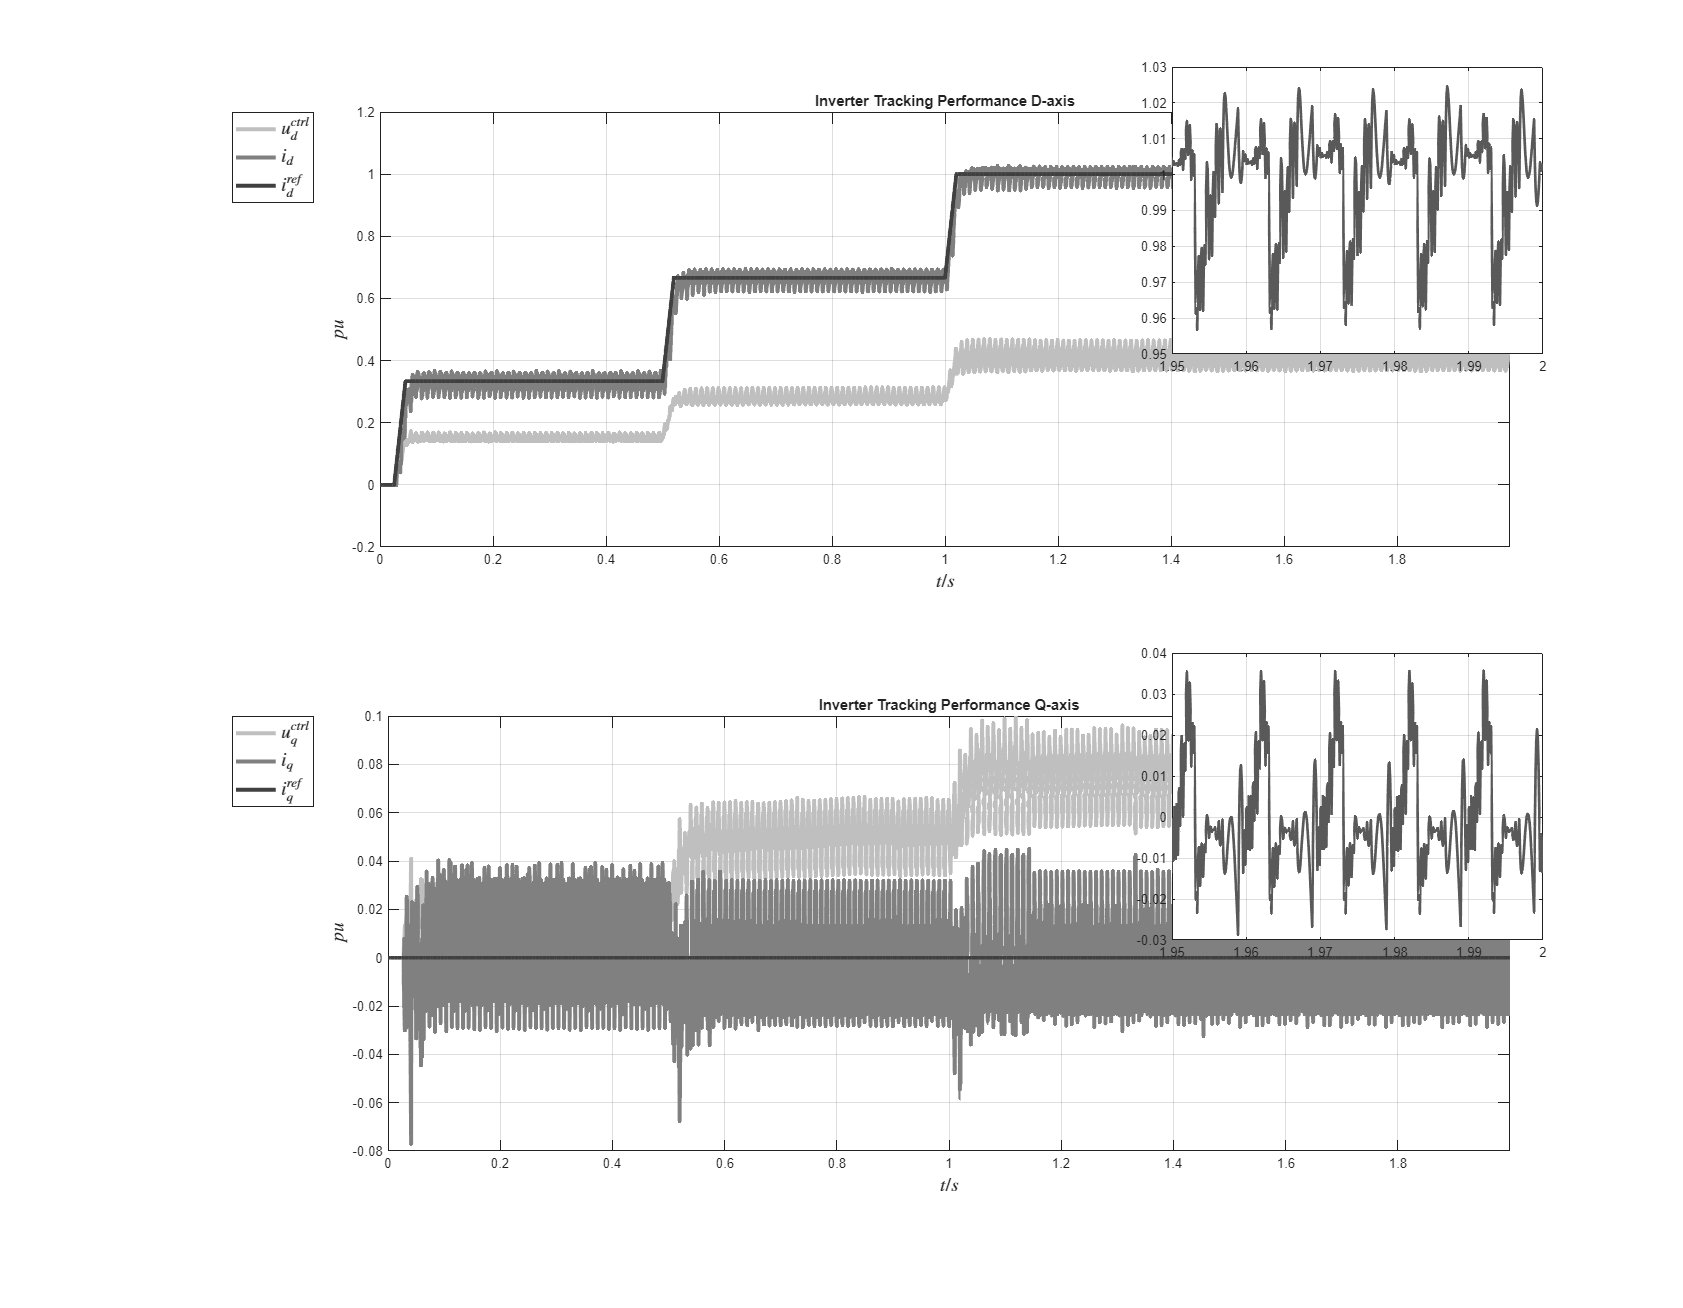
\includegraphics[width =265pt, angle = 0, 
		keepaspectratio]{figures/sim_results_50Hz_10kHz_1/inverter_current_control_1.eps}
		\captionsetup{width=0.65\textwidth, font=footnotesize}	
		\caption{Single phase tracking performance: along D-axis (top), along Q-axis (bottom).}
		\label{inverter_current_control_1}
	\end{subfigure}%
	\begin{subfigure}{0.5\textwidth}
		\centering
		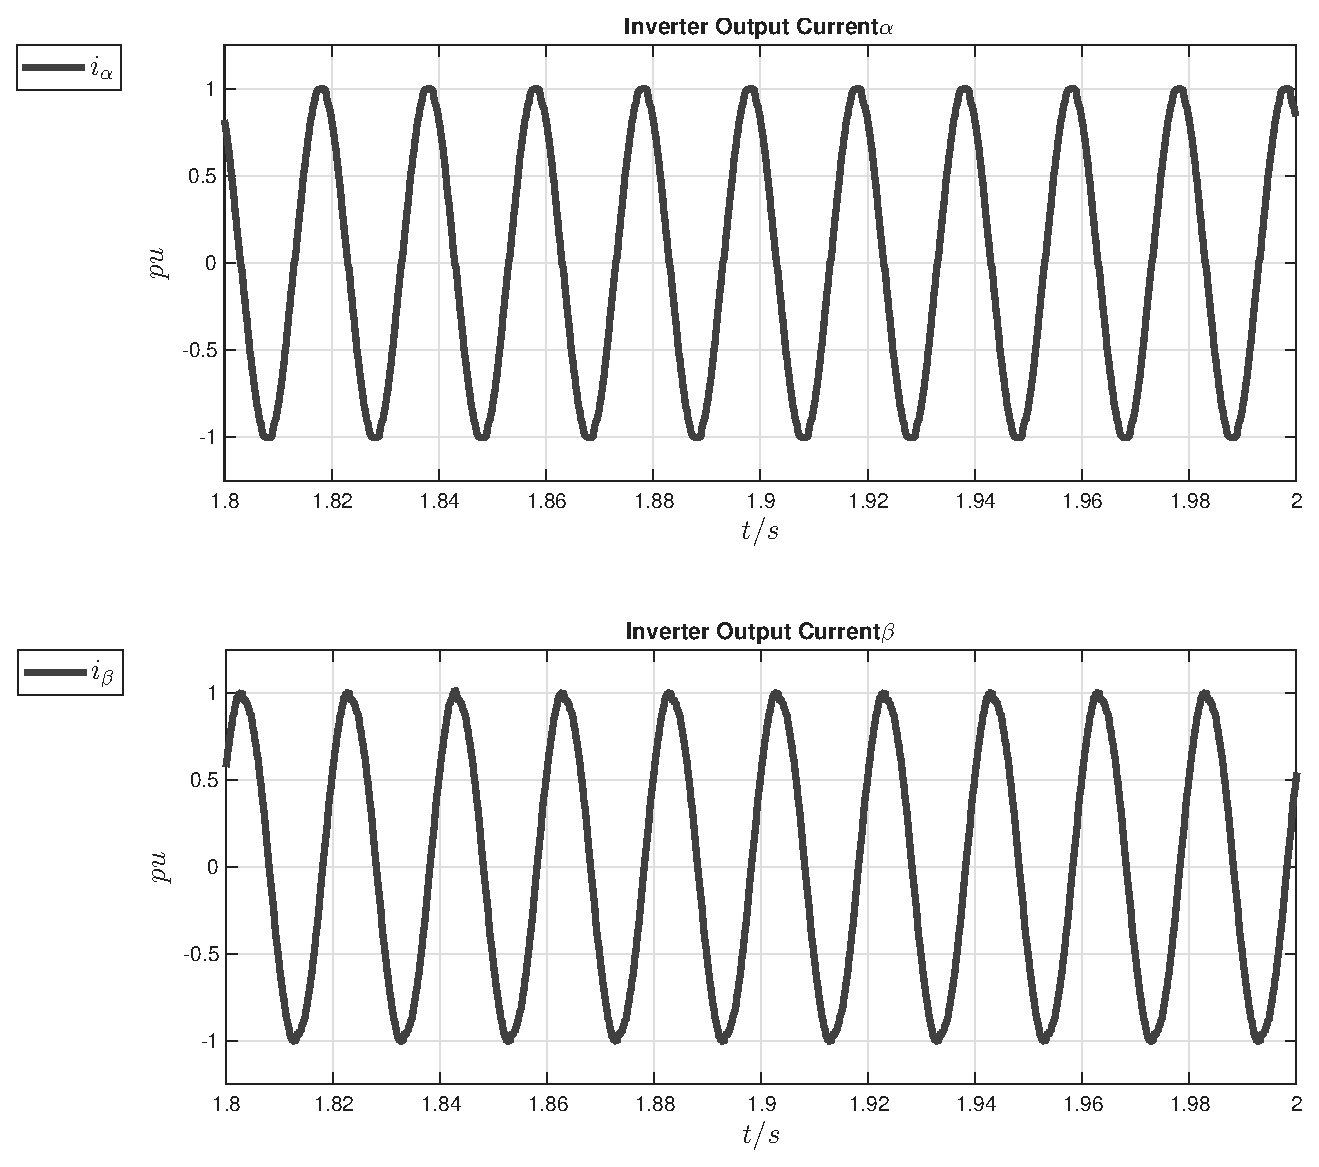
\includegraphics[width =225pt, angle = 0, 
		keepaspectratio]{figures/sim_results_50Hz_10kHz_1/inverter_current_control_2.eps}
		\captionsetup{width=0.75\textwidth, font=footnotesize}	
		\caption{Single phase output current (top), and equivalent shifted by the \textbf{phase-shift-filter} (bottom).}
		\label{inverter_current_control_2}
	\end{subfigure}
	\captionsetup{width=0.65\textwidth, font=small}	
	\caption{Single phase inverter control performance.}
	\label{}
\end{figure}

\begin{figure}[H]
	\centering
	\begin{subfigure}{0.5\textwidth}
		\centering
		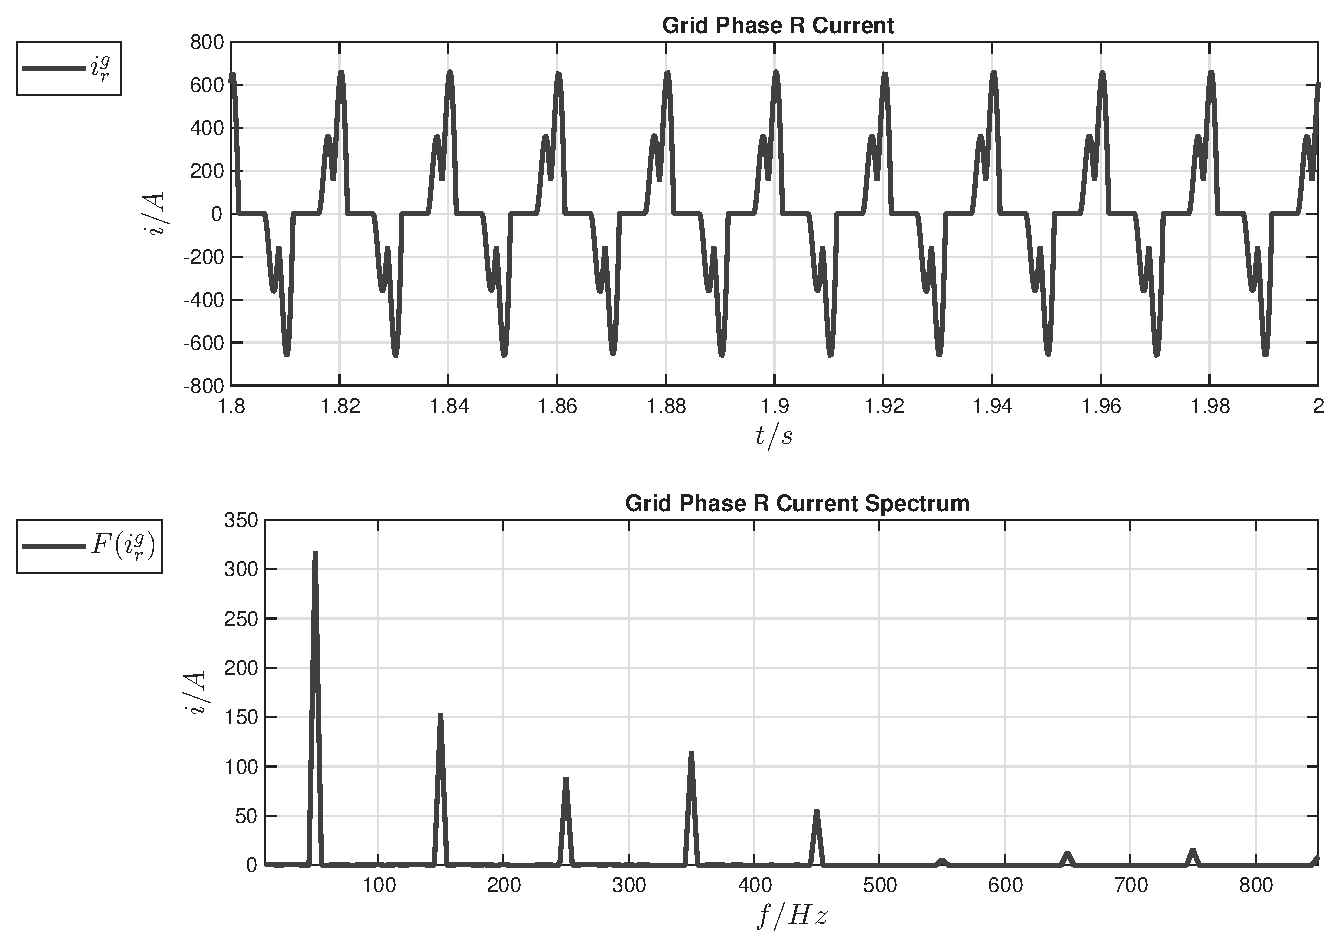
\includegraphics[width = 225pt, angle = 0, 
		keepaspectratio]{figures/sim_results_50Hz_10kHz_1/spectrum_grid_current_r.eps}
		\captionsetup{width=0.65\textwidth, font=footnotesize}	
		\caption{Grid phase current R (top), and grid phase current R spectrum (bottom).}
		\label{spectrum_grid_current_r}
	\end{subfigure}%
	\begin{subfigure}{0.5\textwidth}
		\centering
		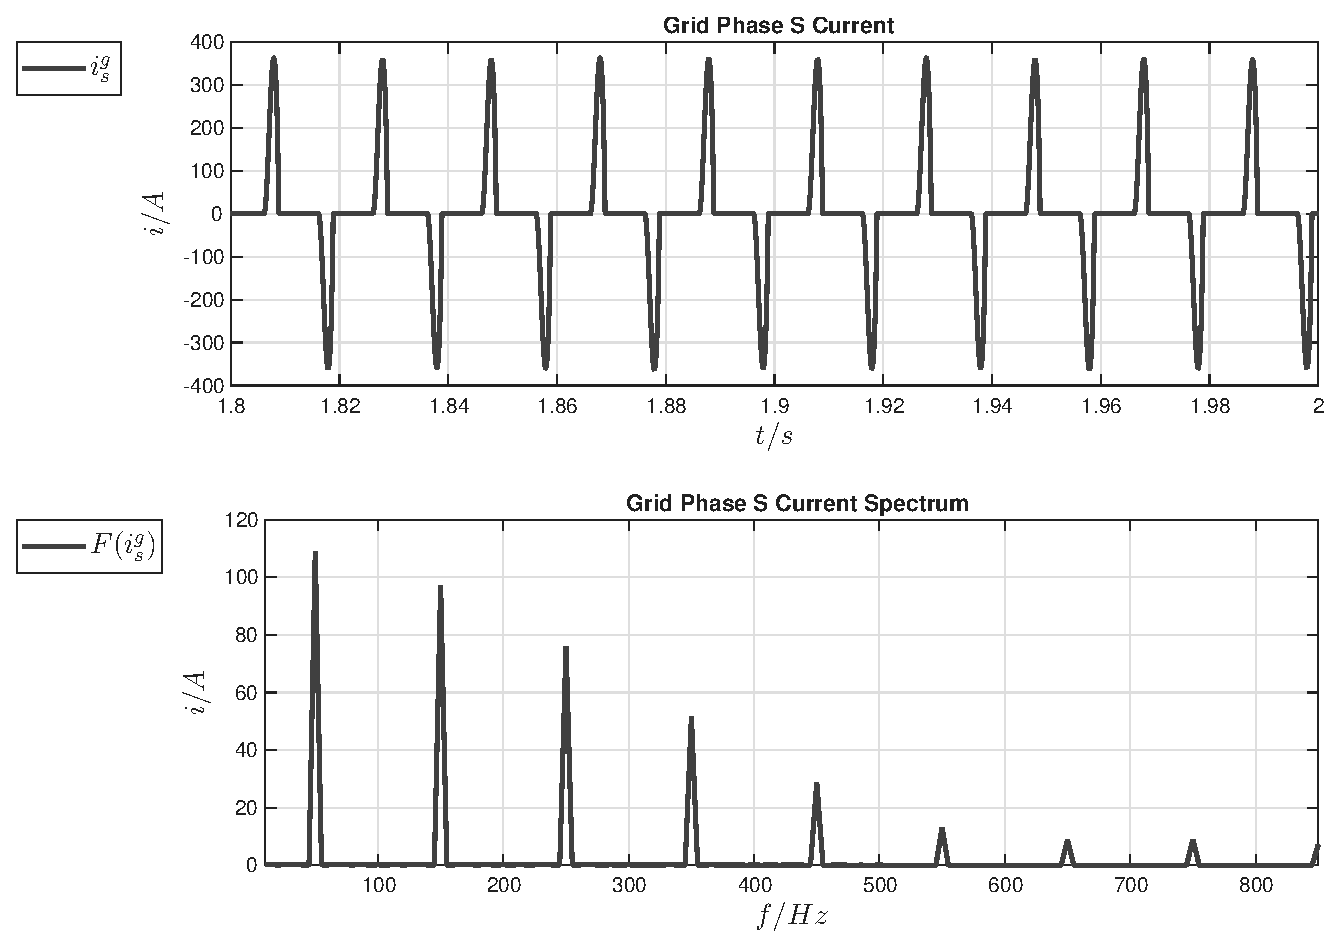
\includegraphics[width =225pt, angle = 0, 
		keepaspectratio]{figures/sim_results_50Hz_10kHz_1/spectrum_grid_current_s.eps}
		\captionsetup{width=0.75\textwidth, font=footnotesize}	
		\caption{Grid phase current S (top), and grid phase current S spectrum (bottom).}
		\label{spectrum_grid_current_s}
	\end{subfigure}
	\captionsetup{width=0.65\textwidth, font=small}	
	\caption{Grid current harmonic analysis.}
	\label{}
\end{figure}

\subsection{Output frequency at 80Hz}

\begin{table}[H]
	%	\footnotesize
	\small
	\begin{center}	
		\begin{tblr}{p{0.75\linewidth}|p{0.25\linewidth}}
			\textbf{Quantity} & \textbf{value} \\
			\hline
			Load current			& $I_m = \SI{45}{\ampere}$ (RMS) \\	
			Load voltage	& $U_{m} = \SI{262}{\ampere}$ (ph-ph RMS) \\	
			Load power factor	& $\cos(\phi) = \SI{0.9}{}$ \\	
			Load fundamental frequency & $f_{load} = \SI{1250}{\hertz}$ \\
			Inverter switching frequency & $f_{sw} = \SI{25}{\kilo\hertz}$ \\
			DC-link voltage & $v_{dc}=\SI{400}{\volt}$ \\
			External gate ON resistance & $R_g^{on}=\SI{6}{\ohm}$ \\			
			External gate OFF resistance & $R_g^{off}=\SI{6}{\ohm}$ \\
			Turn-On Switching Energy ($R_g^{on}=\SI{6}{\ohm}$, $T_j=\SI{125}{\celsius}$, $u_{dc}=\SI{600}{\volt}$, $i_{d}=\SI{80}{\ampere}$) & $E_{on}=\SI{1.56}{\milli\joule}$ \\
			Turn-Off Switching Energy ($R_g^{off}=\SI{6}{\ohm}$, $T_j=\SI{125}{\celsius}$, $u_{dc}=\SI{600}{\volt}$, $i_{d}=\SI{80}{\ampere}$) & $E_{off}=\SI{0.84}{\milli\joule}$ \\
			Reserve Recovery Energy ($T_j=\SI{125}{\celsius}$, $u_{dc}=\SI{600}{\volt}$, $i_{d}=\SI{80}{\ampere}$) & $E_{rr}=\SI{0.075}{\milli\joule}$ \\
			MOSFET Thermal Resistance, Junction to Heatsink (per MOSFET) & $R_{jh}=\SI{0.642}{\celsius\per\watt}$ \\
			Thermal Interface Material (per MOSFET) & $R_{TIM}=\SI{0.5}{\celsius\per\watt}$ \\
			MOSFET Thermal Resistance, Heatsink to Ambient (per MOSFET) & $R_{ha}=\SI{1.88}{\celsius\per\watt}$ \\
			\hline
		\end{tblr}
	\end{center}
	\captionsetup{width=.5\textwidth, font=small}
	\caption{List of condition for the electro-thermal simulation.}
	\label{}
\end{table}	

\begin{figure}[H]
	\centering
	\begin{subfigure}{0.5\textwidth}
		\centering
		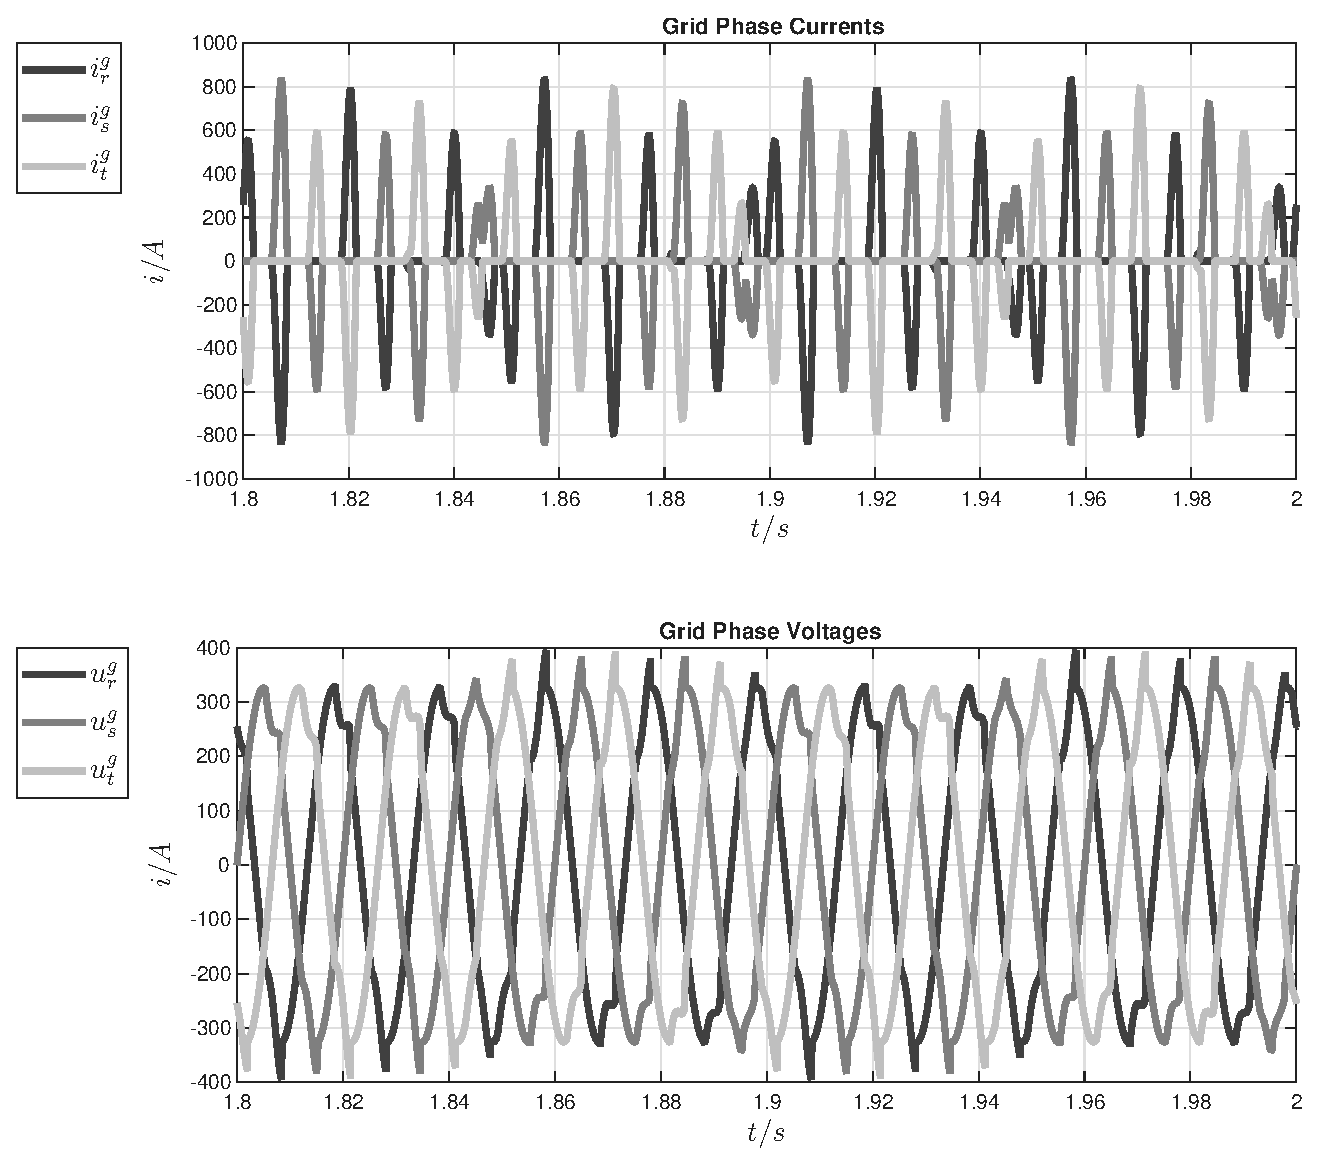
\includegraphics[width =225pt, angle = 0, 
		keepaspectratio]{figures/sim_results_80Hz_10kHz_1/grid_quantities.eps}
		\captionsetup{width=0.75\textwidth, font=footnotesize}	
		\caption{Grid currents (top), and grid voltages (bottom), supposing $S_{nom} = \SI{250}{\kilo\volt\ampere}$ and $U_{cc} = \SI{4}{\percent}$.}
		\label{grid_quantities_80Hz}
	\end{subfigure}%
	\begin{subfigure}{0.5\textwidth}
		\centering
		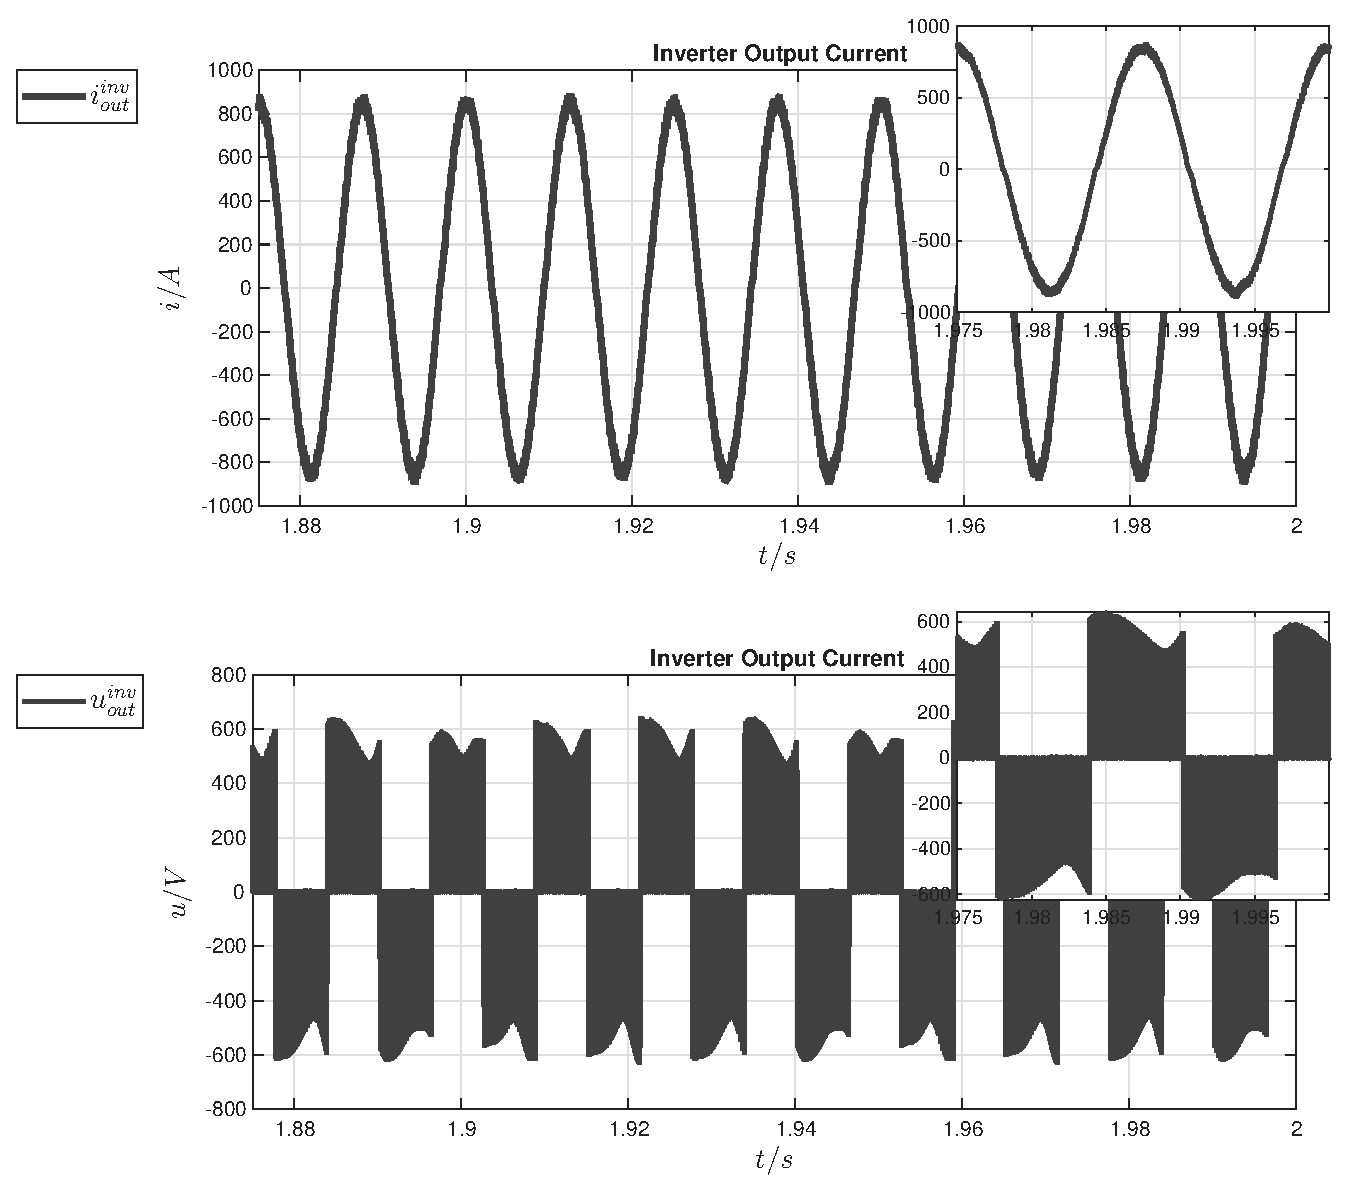
\includegraphics[width =225pt, angle = 0, 
		keepaspectratio]{figures/sim_results_80Hz_10kHz_1/inverter_output_current.eps}
		\captionsetup{width=0.75\textwidth, font=footnotesize}	
		\caption{Inverter output current (top), and inverter output voltage (bottom), supposing $f_{pwm} = \SI{10}{\kilo\hertz}$ per leg.}
		\label{inverter_output_current_80Hz}
	\end{subfigure}
	\captionsetup{width=0.65\textwidth, font=small}	
	\caption{Grid and inverter output quantities.}
	\label{}
\end{figure}

\begin{figure}[H]
	\centering
	\begin{subfigure}{0.5\textwidth}
		\centering
		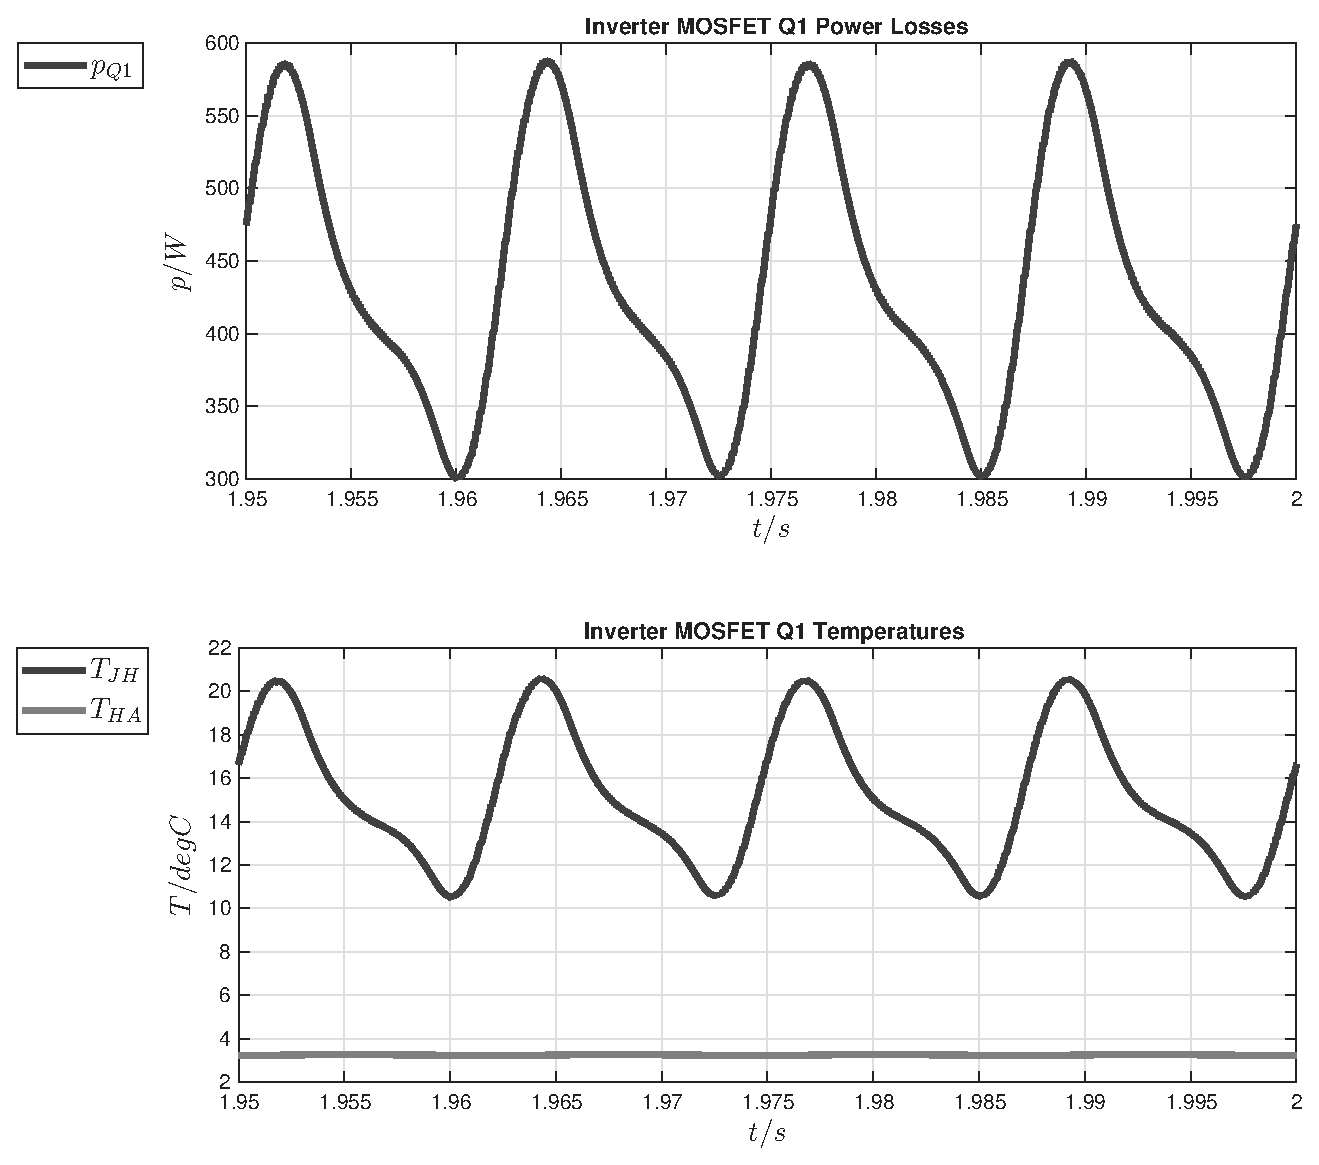
\includegraphics[width =225pt, angle = 0, 
		keepaspectratio]{figures/sim_results_80Hz_10kHz_1/inverter_Q1_power_losses.eps}
		\captionsetup{width=0.65\textwidth, font=footnotesize}	
		\caption{Inverter MOSFET Q1 power loss (top), and junction-case temperature (bottom).}
		\label{inverter_Q1_power_losses_80Hz}
	\end{subfigure}%
	\begin{subfigure}{0.5\textwidth}
		\centering
		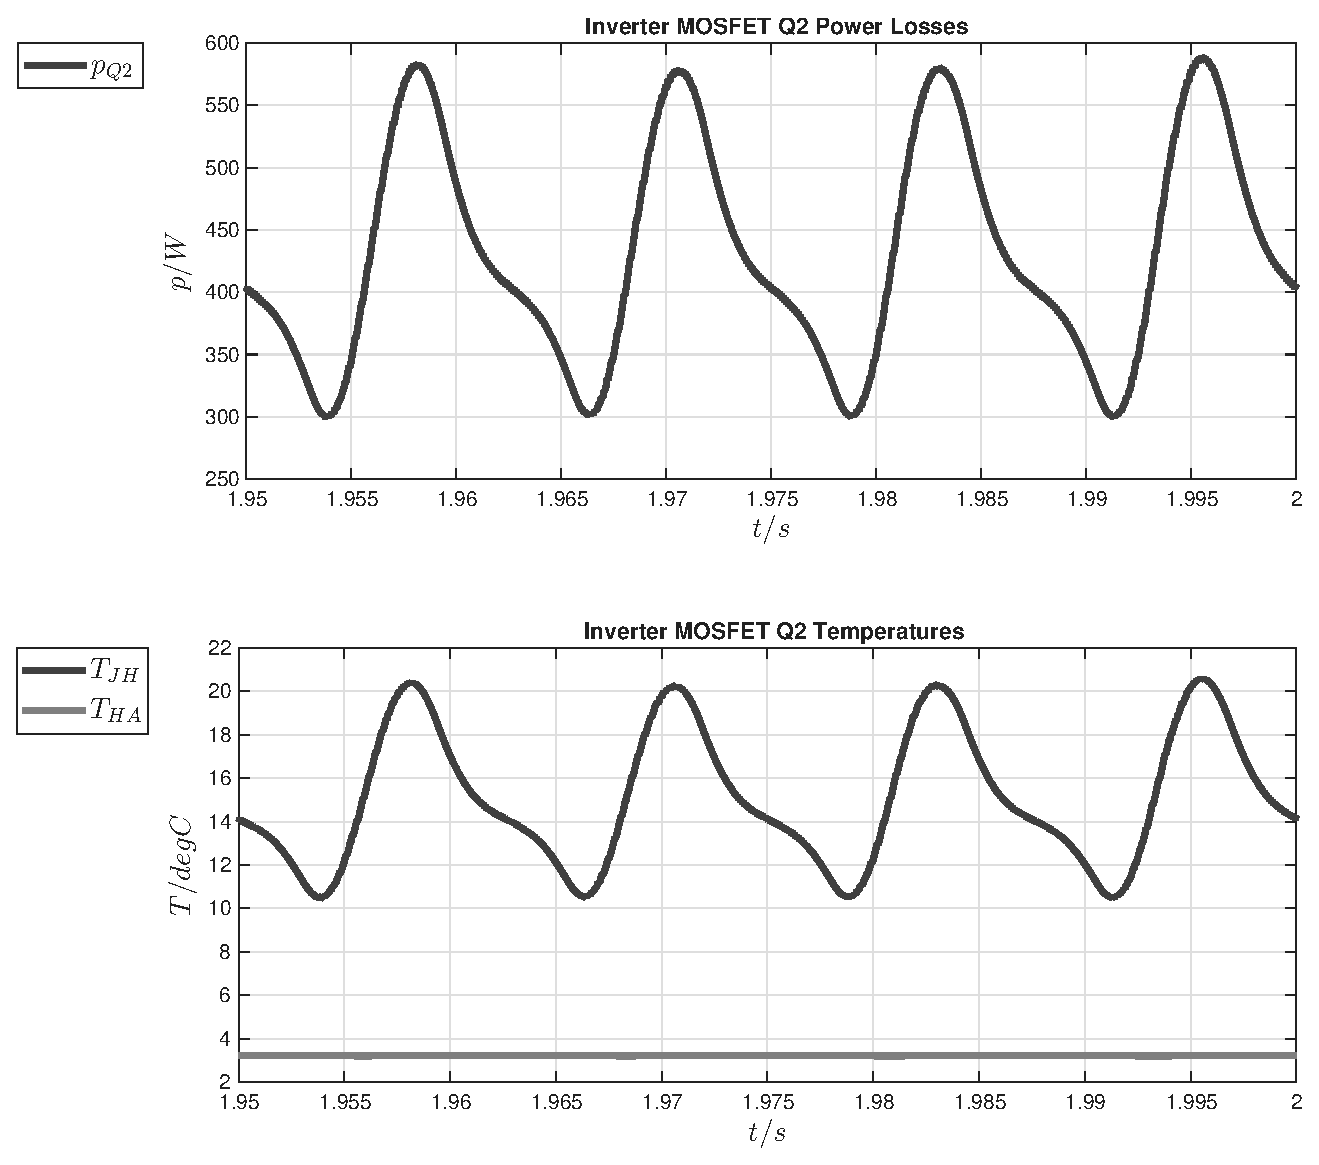
\includegraphics[width =225pt, angle = 0, 
		keepaspectratio]{figures/sim_results_80Hz_10kHz_1/inverter_Q2_power_losses.eps}
		\captionsetup{width=0.75\textwidth, font=footnotesize}	
		\caption{Inverter MOSFET Q2 power loss (top), and junction-case temperature (bottom).}
		\label{inverter_Q2_power_losses_80Hz}
	\end{subfigure}
	\captionsetup{width=0.65\textwidth, font=small}	
	\caption{Inverter MOSFETs thermal performance.}
	\label{}
\end{figure}

\begin{figure}[H]
	\centering
	\begin{subfigure}{0.5\textwidth}
		\centering
		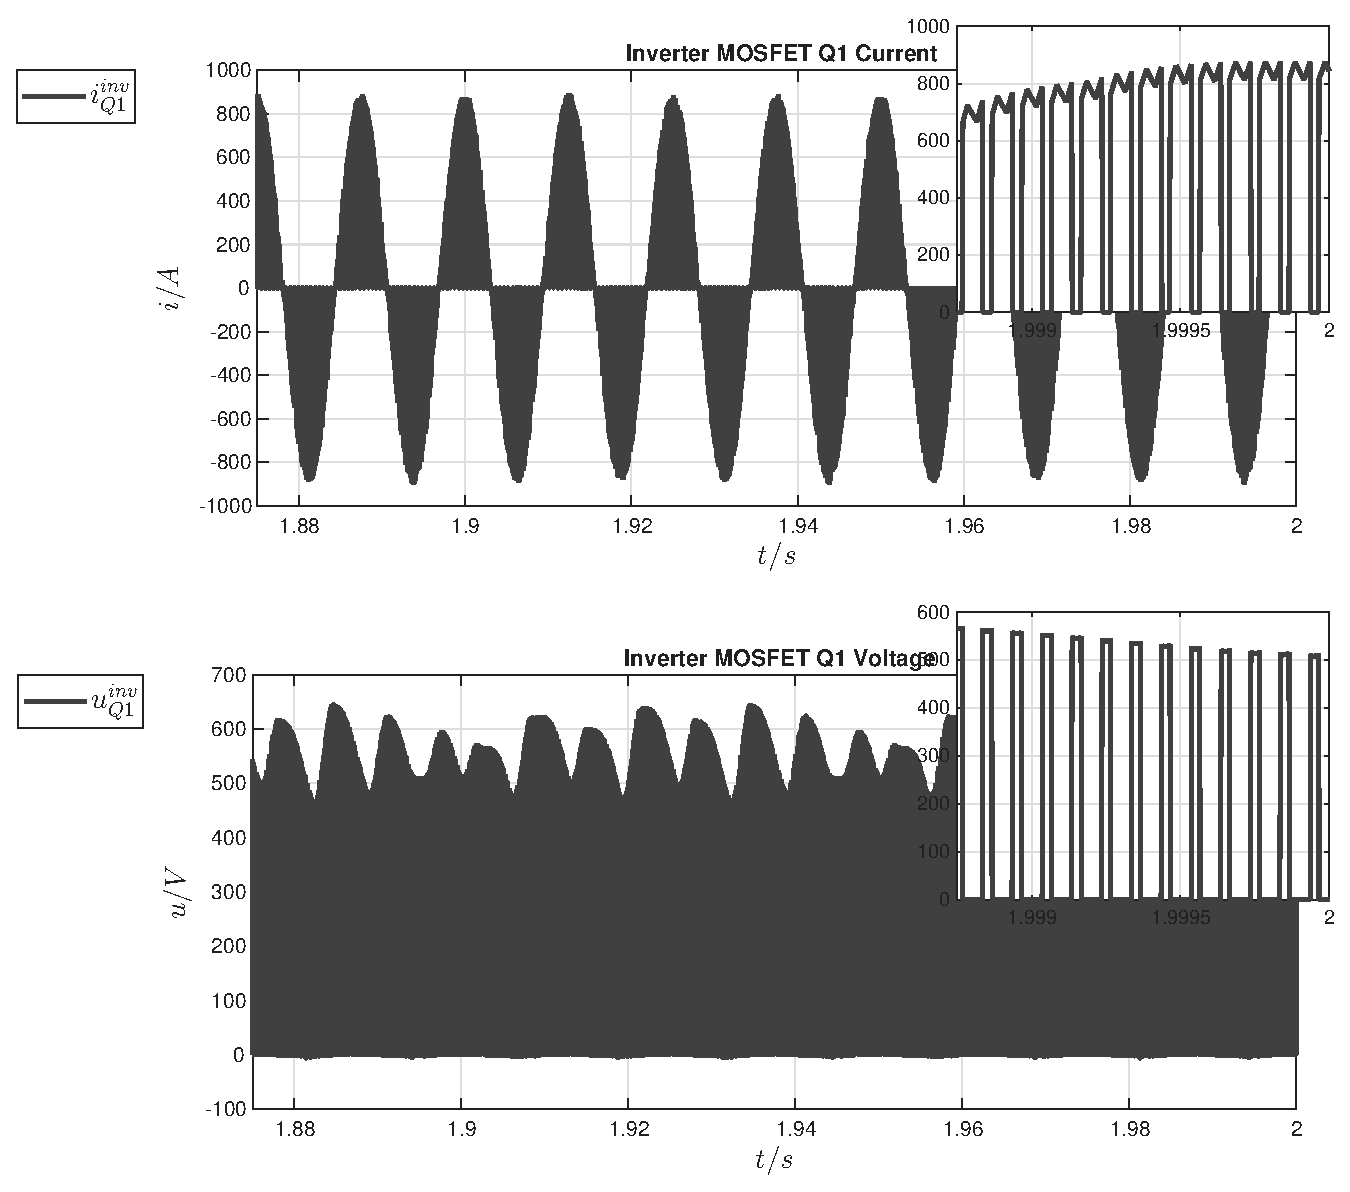
\includegraphics[width =225pt, angle = 0, 
		keepaspectratio]{figures/sim_results_80Hz_10kHz_1/inverter_mosfet_Q1_iu.eps}
		\captionsetup{width=0.65\textwidth, font=footnotesize}	
		\caption{Inverter MOSFET Q1 current (top), and voltage (bottom).}
		\label{inverter_mosfet_Q1_iu_80Hz}
	\end{subfigure}%
	\begin{subfigure}{0.5\textwidth}
		\centering
		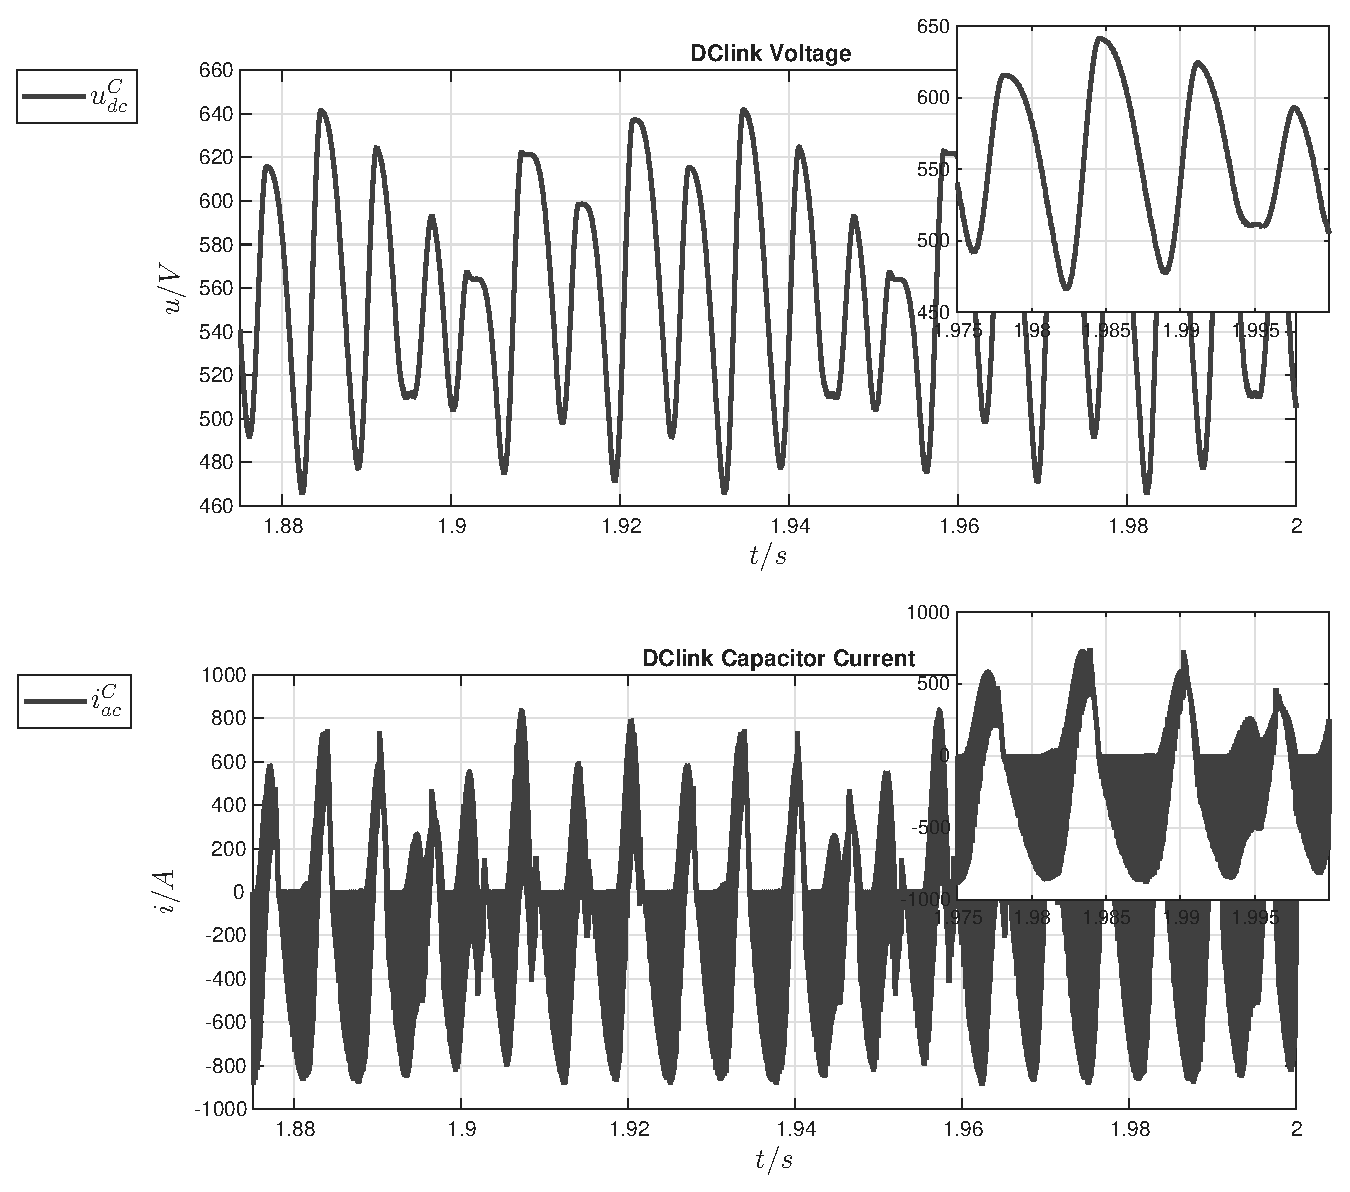
\includegraphics[width =225pt, angle = 0, 
		keepaspectratio]{figures/sim_results_80Hz_10kHz_1/dclink_ui.eps}
		\captionsetup{width=0.75\textwidth, font=footnotesize}	
		\caption{DClink voltage (top), and dclink capcitor current (bottom).}
		\label{dclink_ui_80Hz}
	\end{subfigure}
	\captionsetup{width=0.65\textwidth, font=small}	
	\caption{Inverter MOSFETs, and DClink quantities.}
	\label{}
\end{figure}

\begin{figure}[H]
	\centering
	\begin{subfigure}{0.5\textwidth}
		\centering
		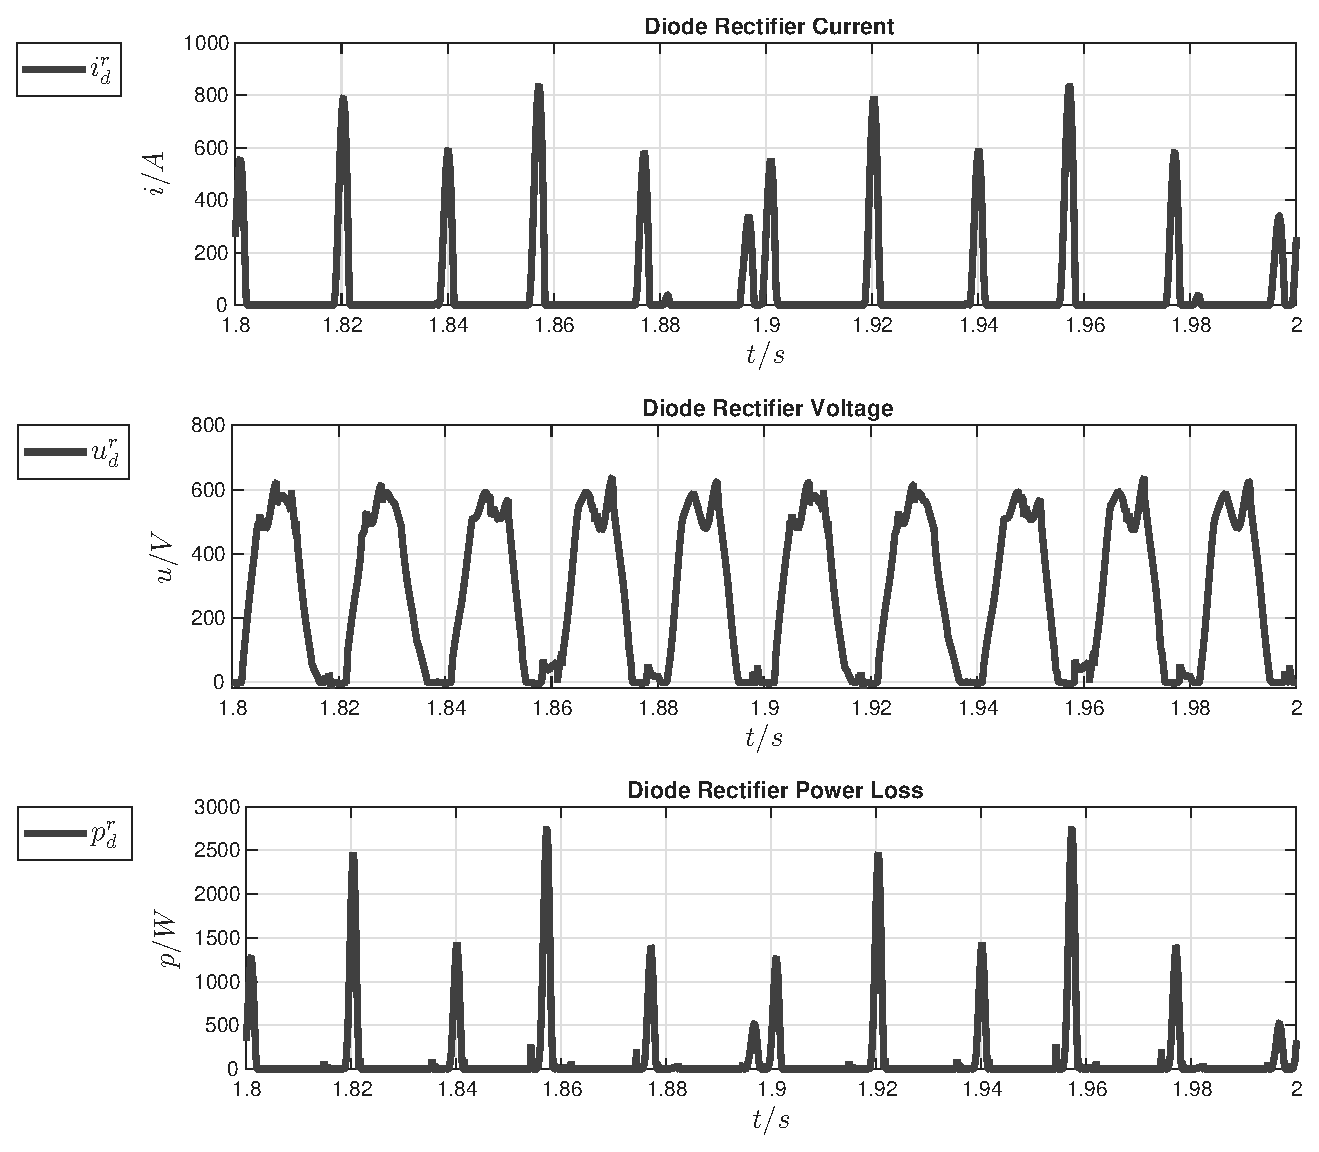
\includegraphics[width =225pt, angle = 0, 
		keepaspectratio]{figures/sim_results_80Hz_10kHz_1/diode_rectifier.eps}
		\captionsetup{width=0.65\textwidth, font=footnotesize}	
		\caption{Diode D1 rectifier current (top), voltage (center), and power loss (bottom).}
		\label{diode_rectifier_80Hz}
	\end{subfigure}%
	\begin{subfigure}{0.5\textwidth}
		\centering
		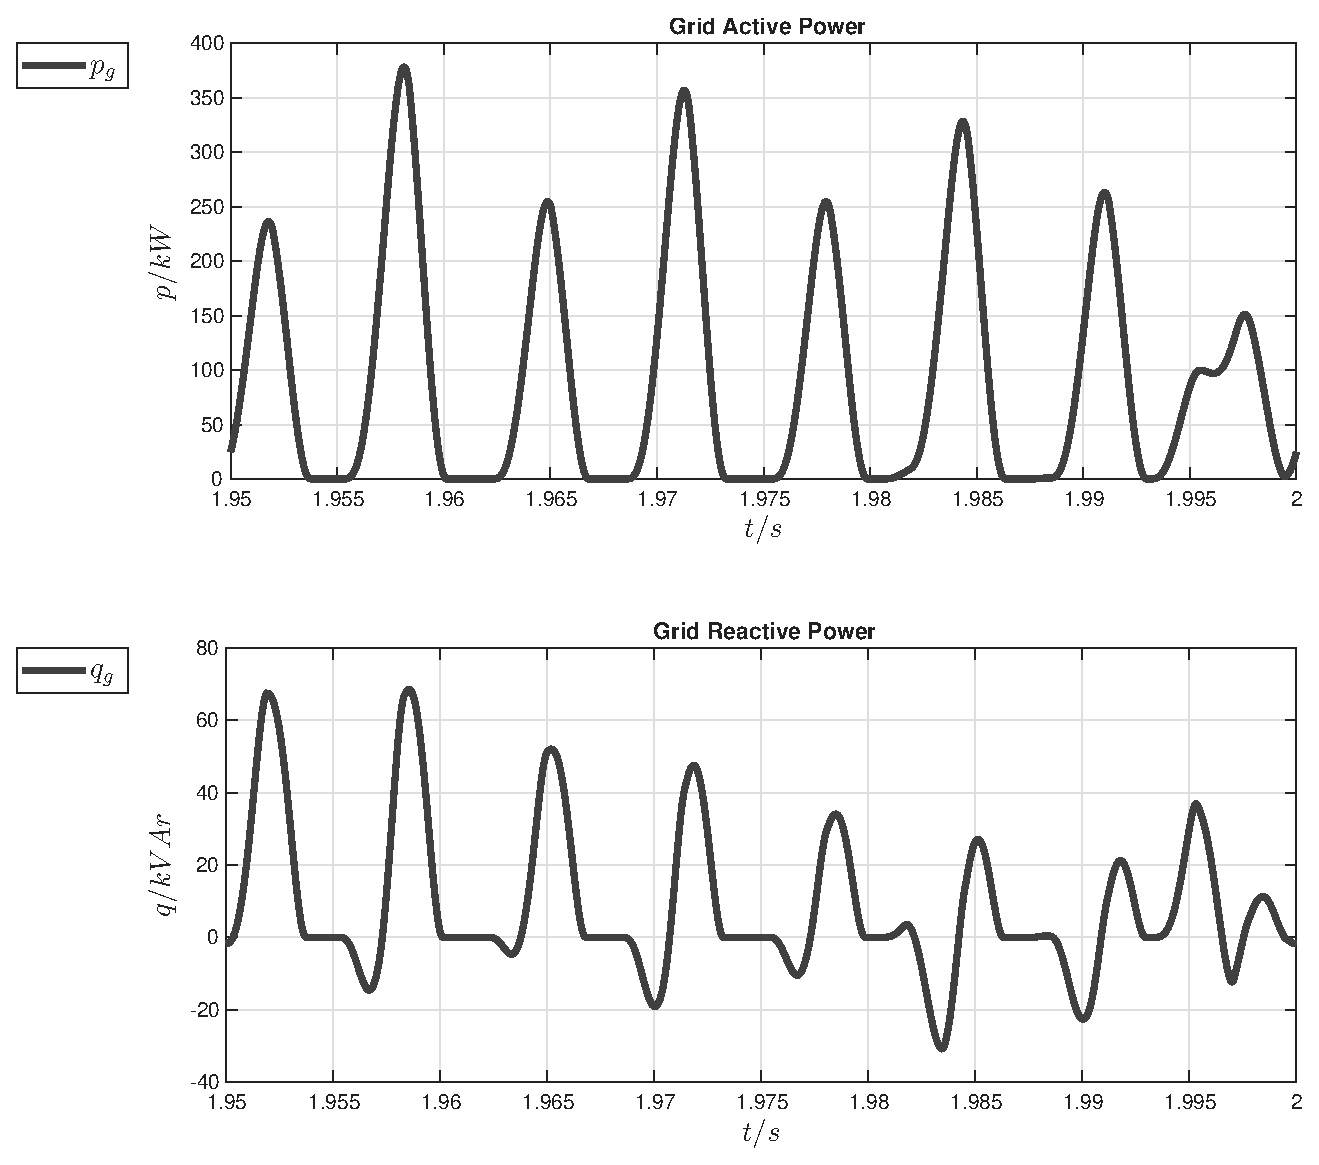
\includegraphics[width =225pt, angle = 0, 
		keepaspectratio]{figures/sim_results_80Hz_10kHz_1/grid_power.eps}
		\captionsetup{width=0.75\textwidth, font=footnotesize}	
		\caption{Grid active power (top), and grid reactive power (bottom) - measure implemented according to IEC.}
		\label{grid_power_80Hz}
	\end{subfigure}
	\captionsetup{width=0.65\textwidth, font=small}	
	\caption{Rectifier diode quantities and grid power analysis.}
	\label{}
\end{figure}

\begin{figure}[H]
	\centering
	\begin{subfigure}{0.5\textwidth}
		\centering
		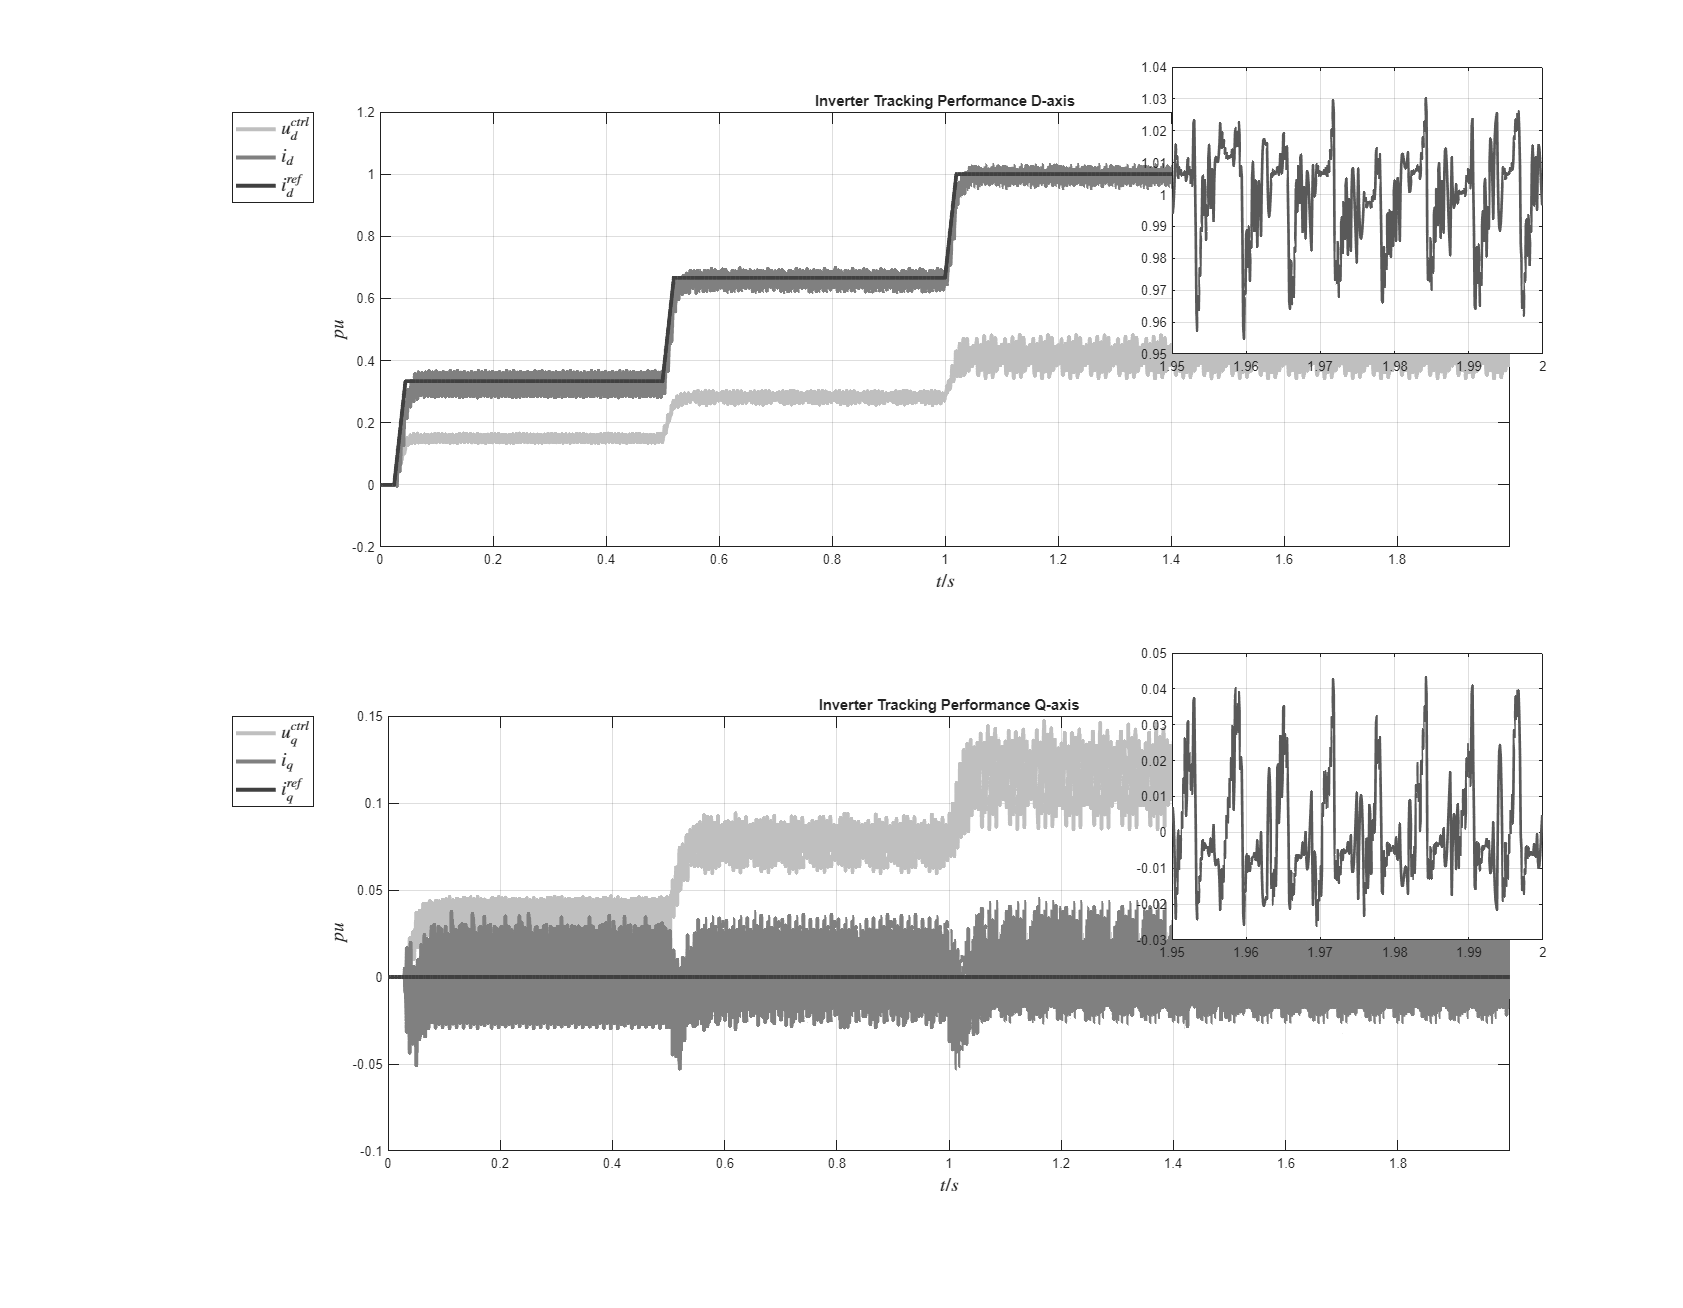
\includegraphics[width =265pt, angle = 0, 
		keepaspectratio]{figures/sim_results_80Hz_10kHz_1/inverter_current_control_1.eps}
		\captionsetup{width=0.65\textwidth, font=footnotesize}	
		\caption{Single phase tracking performance: along D-axis (top), along Q-axis (bottom).}
		\label{inverter_current_control_1_80Hz}
	\end{subfigure}%
	\begin{subfigure}{0.5\textwidth}
		\centering
		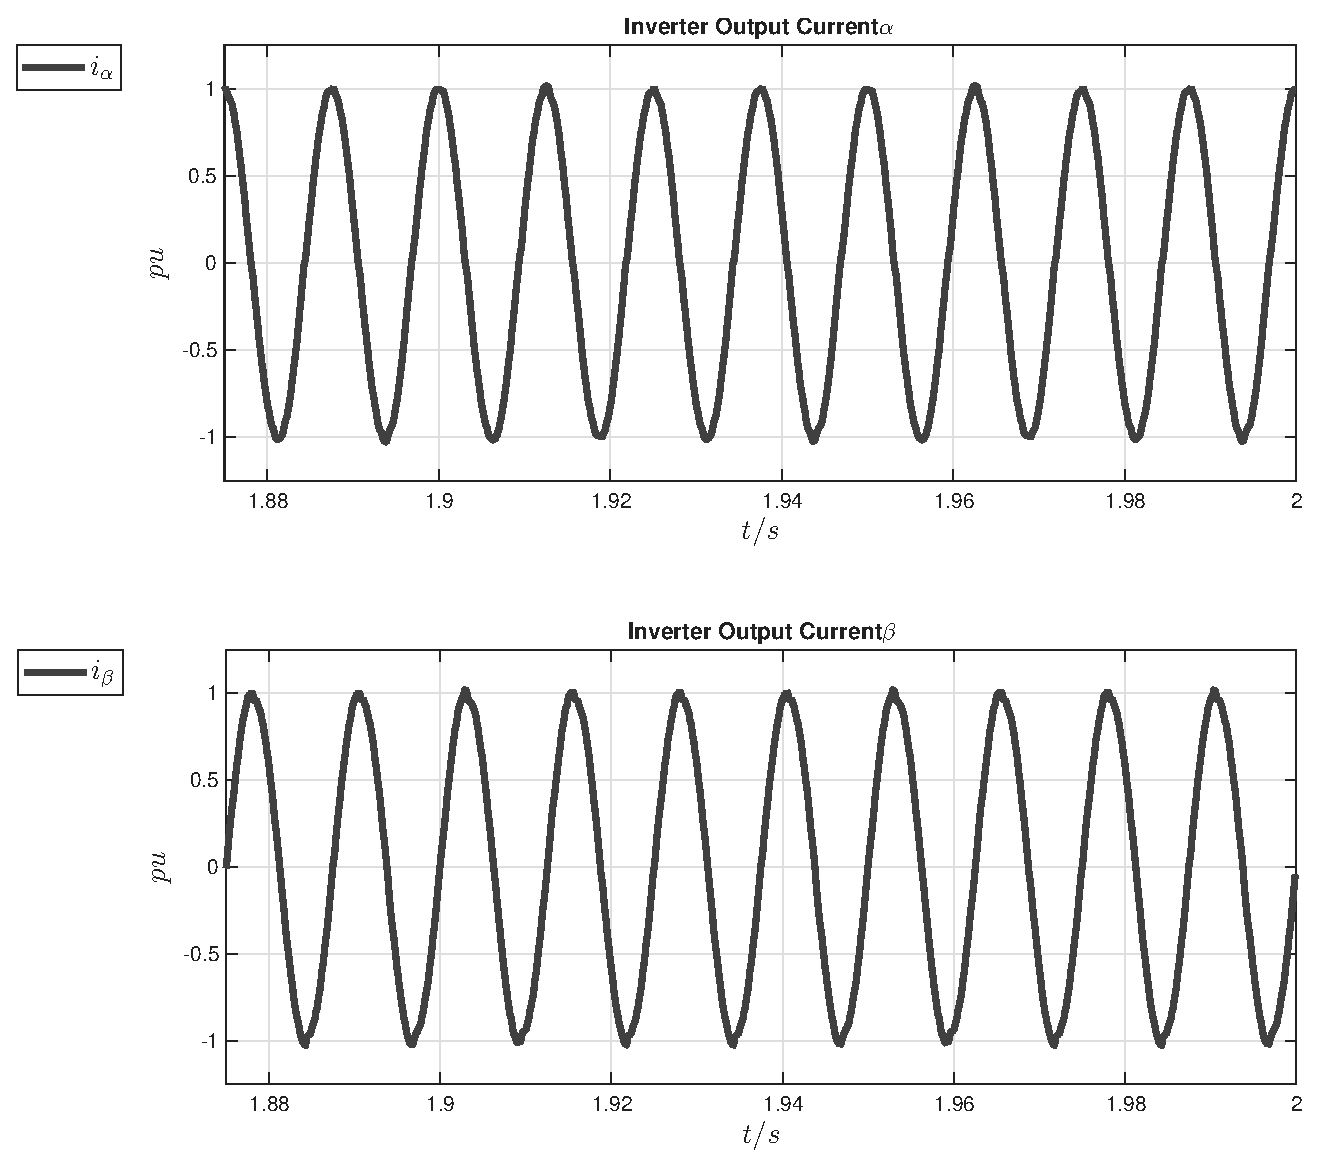
\includegraphics[width =225pt, angle = 0, 
		keepaspectratio]{figures/sim_results_80Hz_10kHz_1/inverter_current_control_2.eps}
		\captionsetup{width=0.75\textwidth, font=footnotesize}	
		\caption{Single phase output current (top), and equivalent shifted by the \textbf{phase-shift-filter} (bottom).}
		\label{inverter_current_control_2_80Hz}
	\end{subfigure}
	\captionsetup{width=0.65\textwidth, font=small}	
	\caption{Single phase inverter control performance.}
	\label{}
\end{figure}

\begin{figure}[H]
	\centering
	\begin{subfigure}{0.5\textwidth}
		\centering
		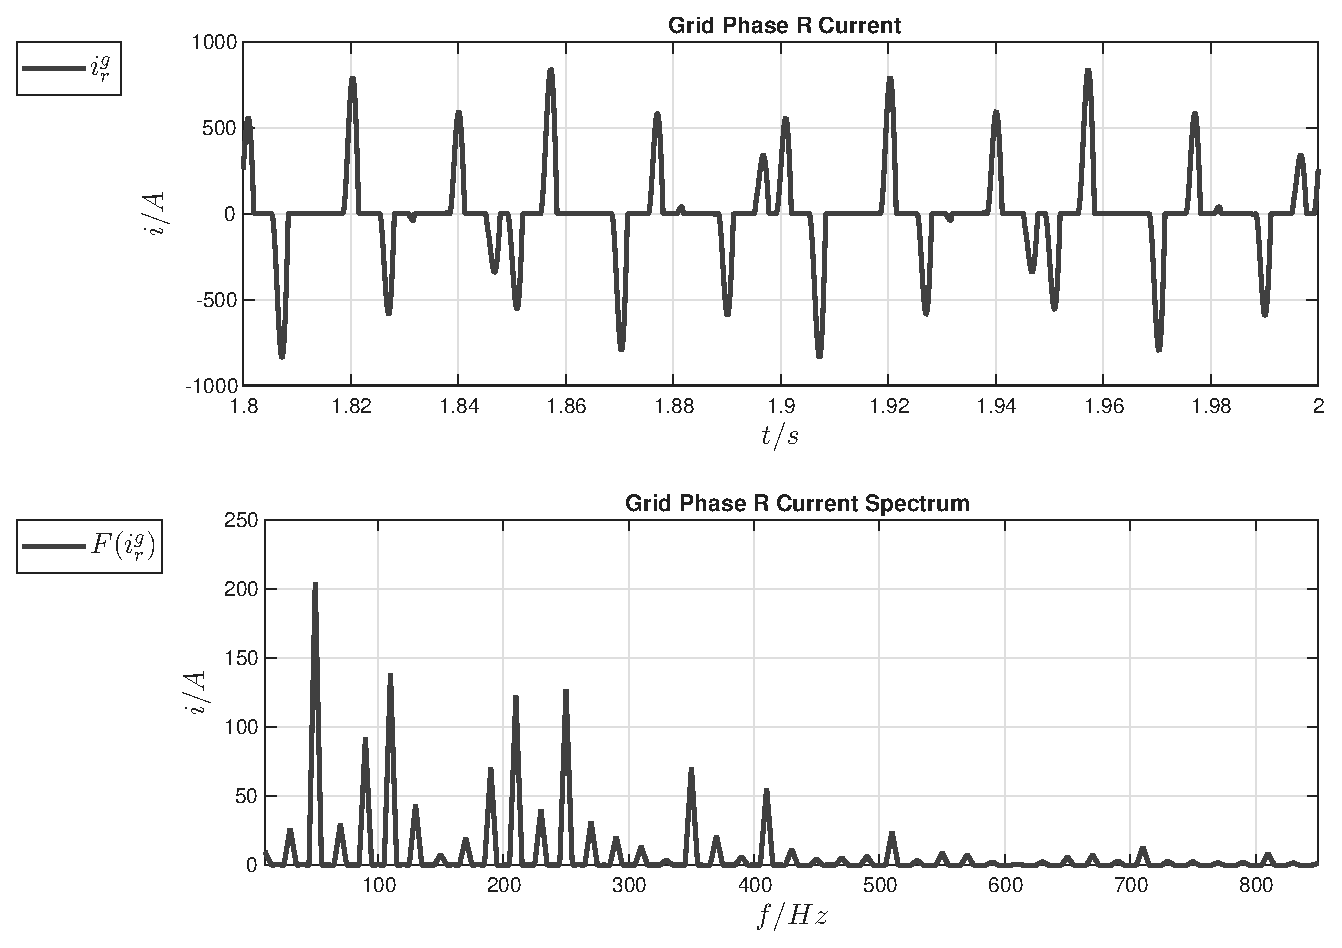
\includegraphics[width = 225pt, angle = 0, 
		keepaspectratio]{figures/sim_results_80Hz_10kHz_1/spectrum_grid_current_r.eps}
		\captionsetup{width=0.65\textwidth, font=footnotesize}	
		\caption{Grid phase current R (top), and grid phase current R spectrum (bottom).}
		\label{spectrum_grid_current_r_80Hz}
	\end{subfigure}%
	\begin{subfigure}{0.5\textwidth}
		\centering
		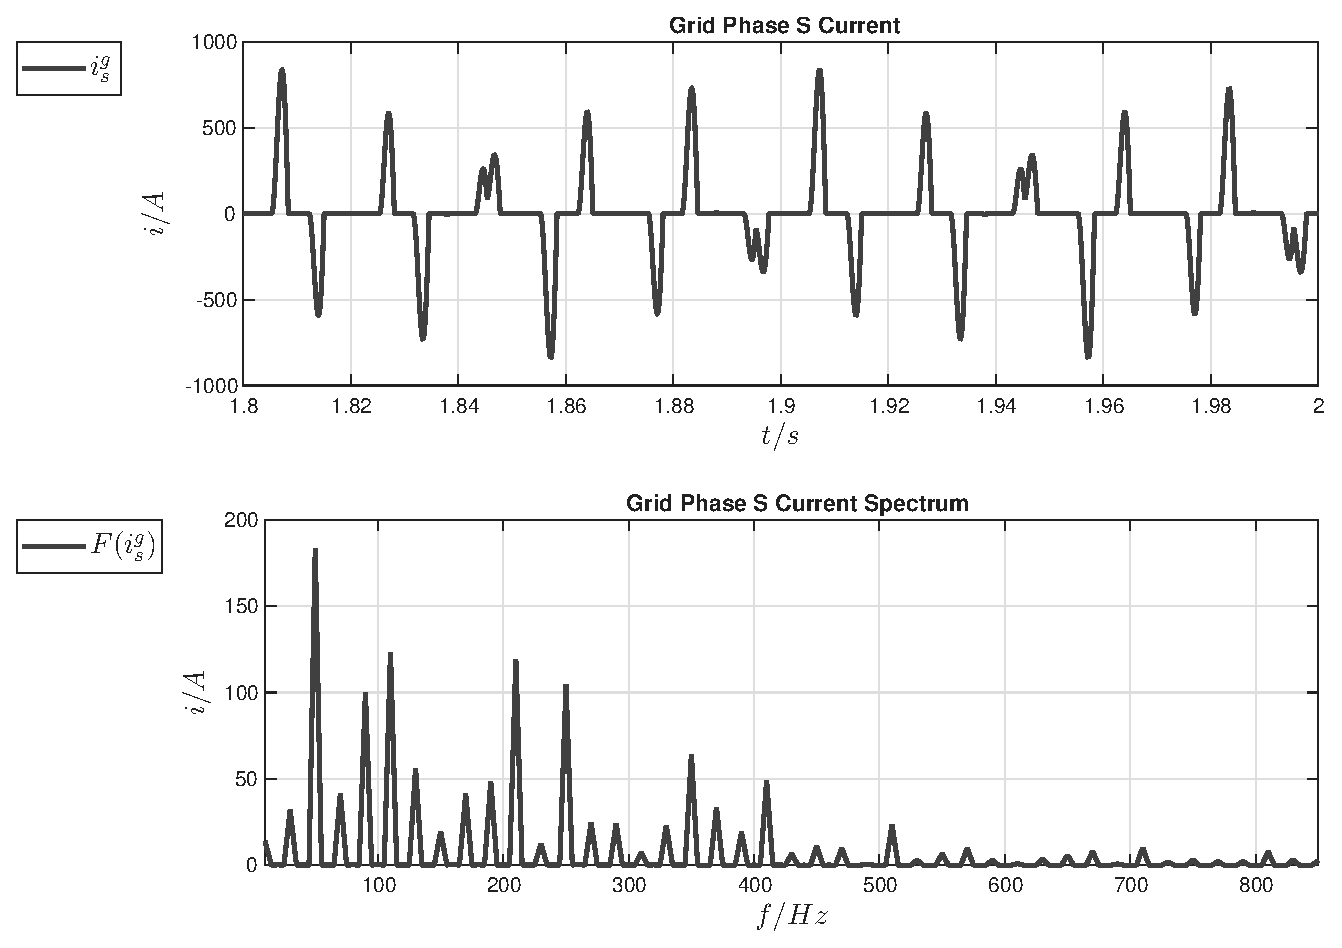
\includegraphics[width =225pt, angle = 0, 
		keepaspectratio]{figures/sim_results_80Hz_10kHz_1/spectrum_grid_current_s.eps}
		\captionsetup{width=0.75\textwidth, font=footnotesize}	
		\caption{Grid phase current S (top), and grid phase current S spectrum (bottom).}
		\label{spectrum_grid_current_s_80Hz}
	\end{subfigure}
	\captionsetup{width=0.65\textwidth, font=small}	
	\caption{Grid current harmonic analysis.}
	\label{}
\end{figure}

\subsection{Output frequency at 400Hz}

\begin{table}[H]
	%	\footnotesize
	\small
	\begin{center}	
		\begin{tblr}{p{0.75\linewidth}|p{0.25\linewidth}}
			\textbf{Quantity} & \textbf{value} \\
			\hline
			Load current			& $I_m = \SI{45}{\ampere}$ (RMS) \\	
			Load voltage	& $U_{m} = \SI{262}{\ampere}$ (ph-ph RMS) \\	
			Load power factor	& $\cos(\phi) = \SI{0.9}{}$ \\	
			Load fundamental frequency & $f_{load} = \SI{1250}{\hertz}$ \\
			Inverter switching frequency & $f_{sw} = \SI{25}{\kilo\hertz}$ \\
			DC-link voltage & $v_{dc}=\SI{400}{\volt}$ \\
			External gate ON resistance & $R_g^{on}=\SI{6}{\ohm}$ \\			
			External gate OFF resistance & $R_g^{off}=\SI{6}{\ohm}$ \\
			Turn-On Switching Energy ($R_g^{on}=\SI{6}{\ohm}$, $T_j=\SI{125}{\celsius}$, $u_{dc}=\SI{600}{\volt}$, $i_{d}=\SI{80}{\ampere}$) & $E_{on}=\SI{1.56}{\milli\joule}$ \\
			Turn-Off Switching Energy ($R_g^{off}=\SI{6}{\ohm}$, $T_j=\SI{125}{\celsius}$, $u_{dc}=\SI{600}{\volt}$, $i_{d}=\SI{80}{\ampere}$) & $E_{off}=\SI{0.84}{\milli\joule}$ \\
			Reserve Recovery Energy ($T_j=\SI{125}{\celsius}$, $u_{dc}=\SI{600}{\volt}$, $i_{d}=\SI{80}{\ampere}$) & $E_{rr}=\SI{0.075}{\milli\joule}$ \\
			MOSFET Thermal Resistance, Junction to Heatsink (per MOSFET) & $R_{jh}=\SI{0.642}{\celsius\per\watt}$ \\
			Thermal Interface Material (per MOSFET) & $R_{TIM}=\SI{0.5}{\celsius\per\watt}$ \\
			MOSFET Thermal Resistance, Heatsink to Ambient (per MOSFET) & $R_{ha}=\SI{1.88}{\celsius\per\watt}$ \\
			\hline
		\end{tblr}
	\end{center}
	\captionsetup{width=.5\textwidth, font=small}
	\caption{List of condition for the electro-thermal simulation.}
	\label{}
\end{table}	

\begin{figure}[H]
	\centering
	\begin{subfigure}{0.5\textwidth}
		\centering
		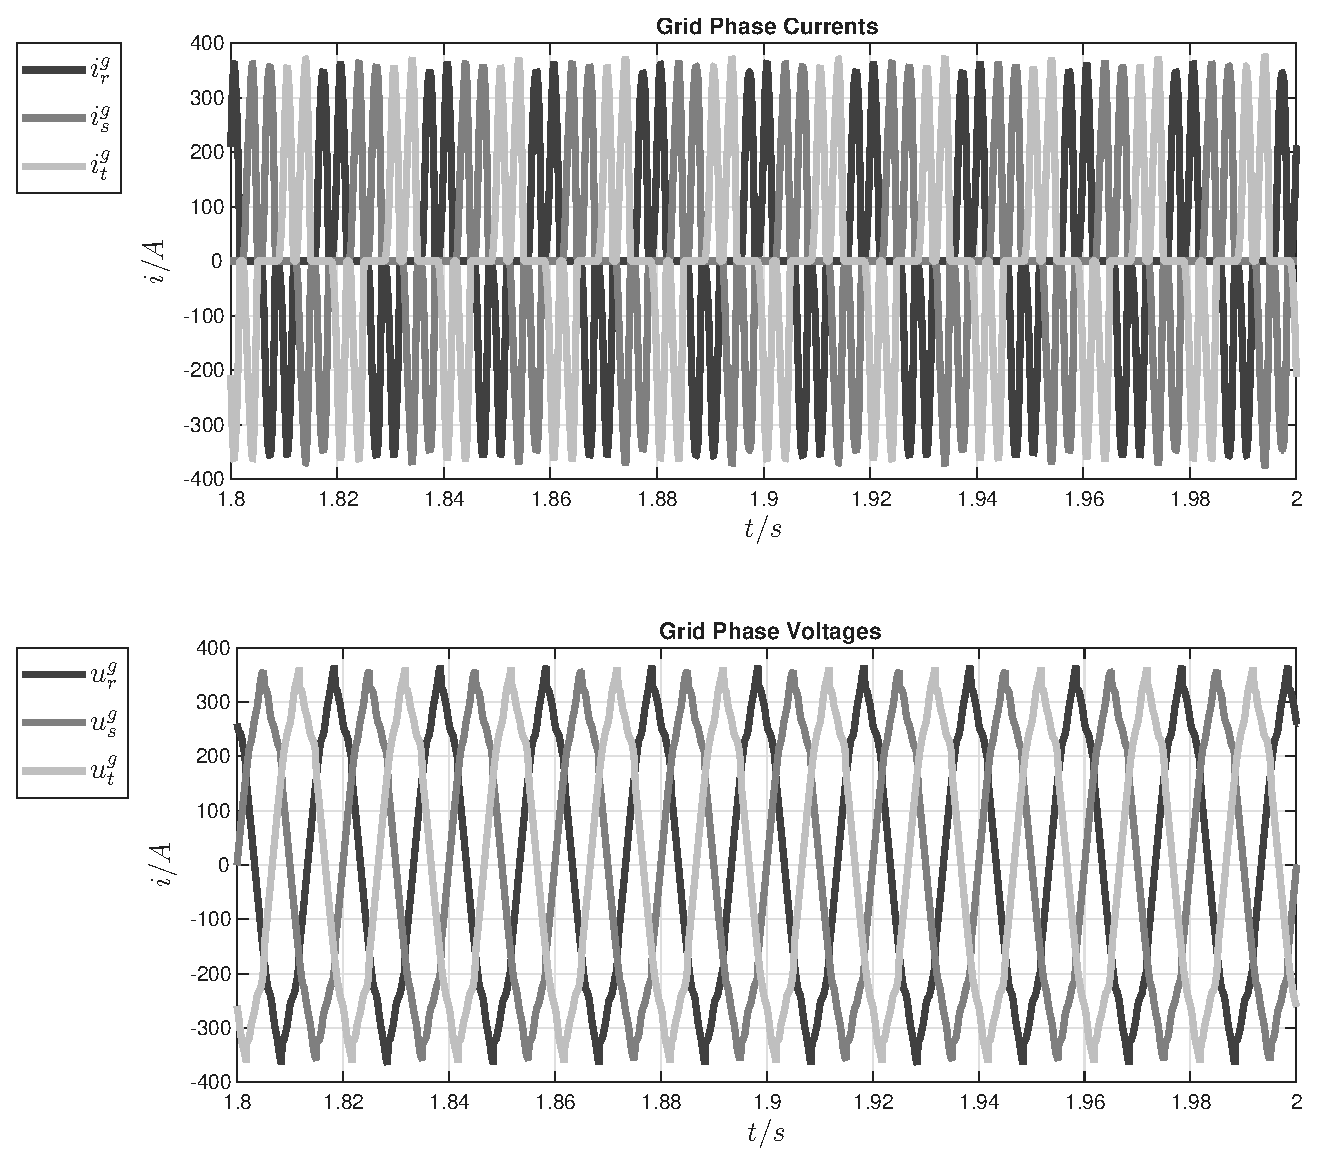
\includegraphics[width =225pt, angle = 0, 
		keepaspectratio]{figures/sim_results_400Hz_10kHz_1/grid_quantities.eps}
		\captionsetup{width=0.75\textwidth, font=footnotesize}	
		\caption{Grid currents (top), and grid voltages (bottom), supposing $S_{nom} = \SI{250}{\kilo\volt\ampere}$ and $U_{cc} = \SI{4}{\percent}$.}
		\label{grid_quantities_400Hz}
	\end{subfigure}%
	\begin{subfigure}{0.5\textwidth}
		\centering
		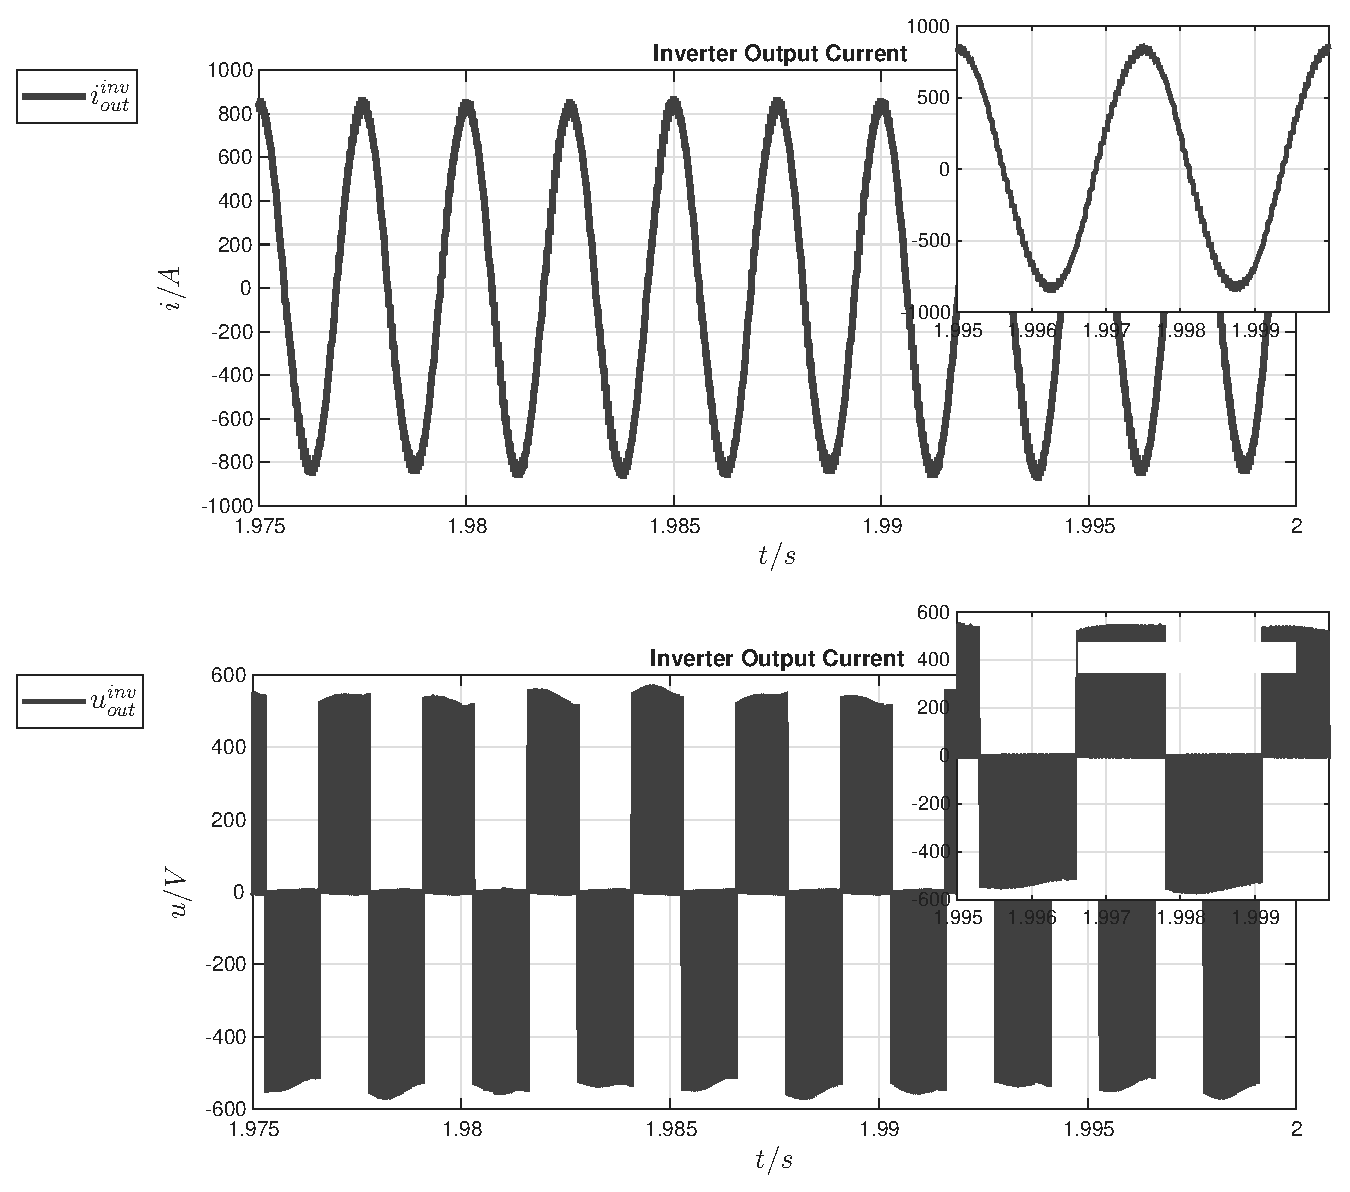
\includegraphics[width =225pt, angle = 0, 
		keepaspectratio]{figures/sim_results_400Hz_10kHz_1/inverter_output_current.eps}
		\captionsetup{width=0.75\textwidth, font=footnotesize}	
		\caption{Inverter output current (top), and inverter output voltage (bottom), supposing $f_{pwm} = \SI{10}{\kilo\hertz}$ per leg.}
		\label{inverter_output_current_400Hz}
	\end{subfigure}
	\captionsetup{width=0.65\textwidth, font=small}	
	\caption{Grid and inverter output quantities.}
	\label{}
\end{figure}

\begin{figure}[H]
	\centering
	\begin{subfigure}{0.5\textwidth}
		\centering
		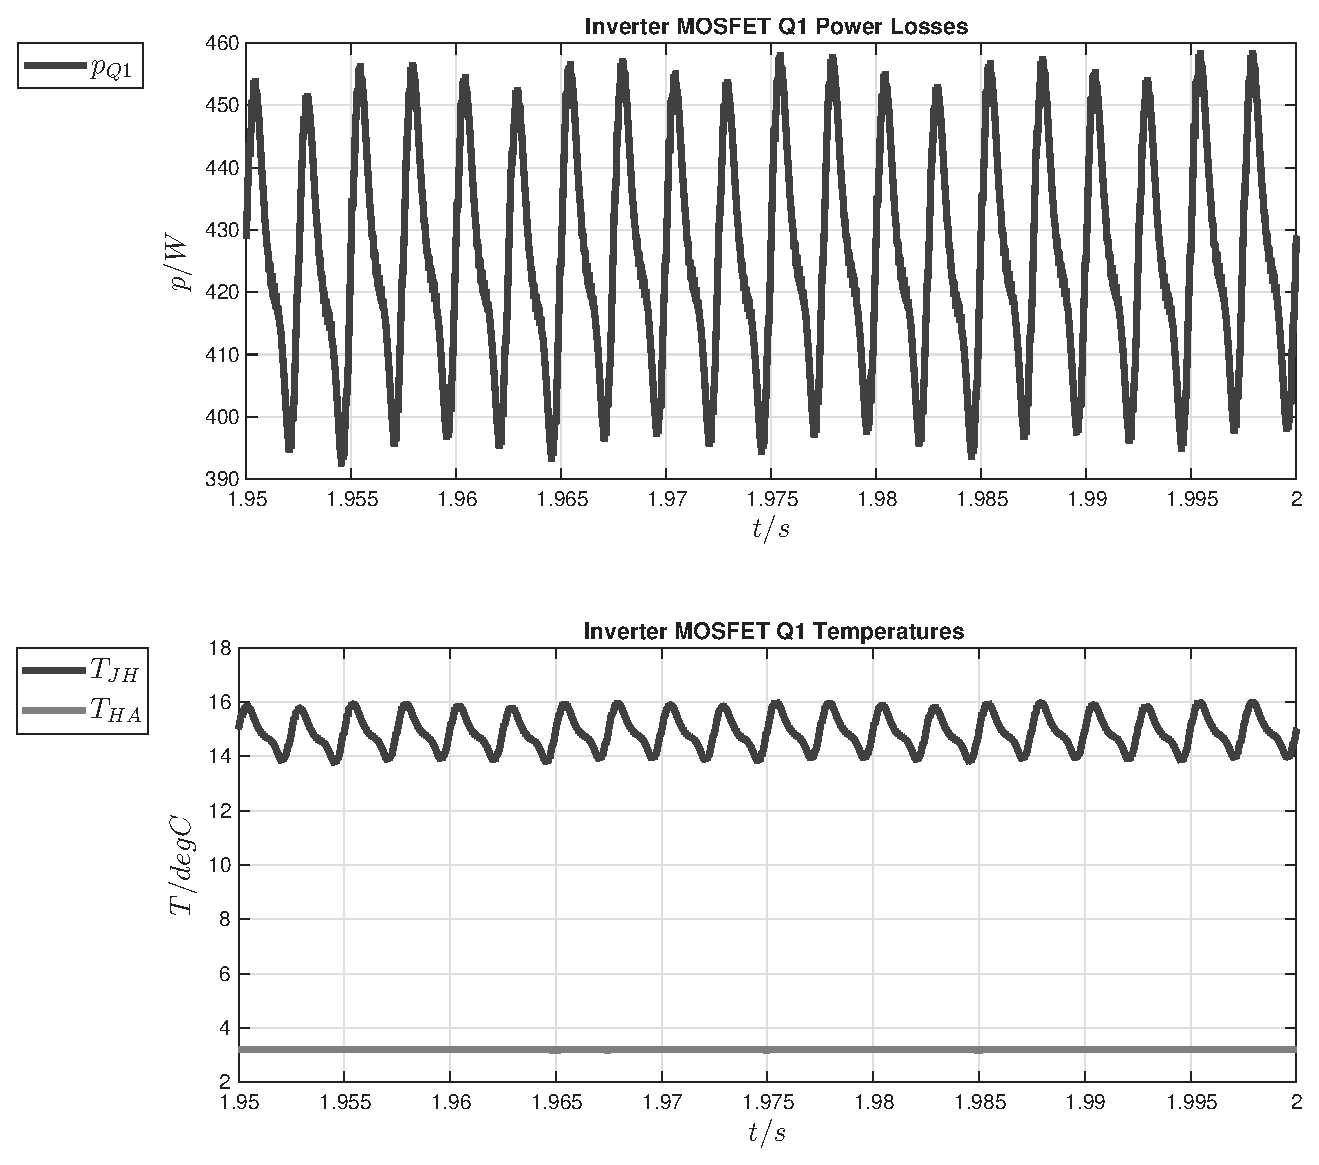
\includegraphics[width =225pt, angle = 0, 
		keepaspectratio]{figures/sim_results_400Hz_10kHz_1/inverter_Q1_power_losses.eps}
		\captionsetup{width=0.65\textwidth, font=footnotesize}	
		\caption{Inverter MOSFET Q1 power loss (top), and junction-case temperature (bottom).}
		\label{inverter_Q1_power_losses_400Hz}
	\end{subfigure}%
	\begin{subfigure}{0.5\textwidth}
		\centering
		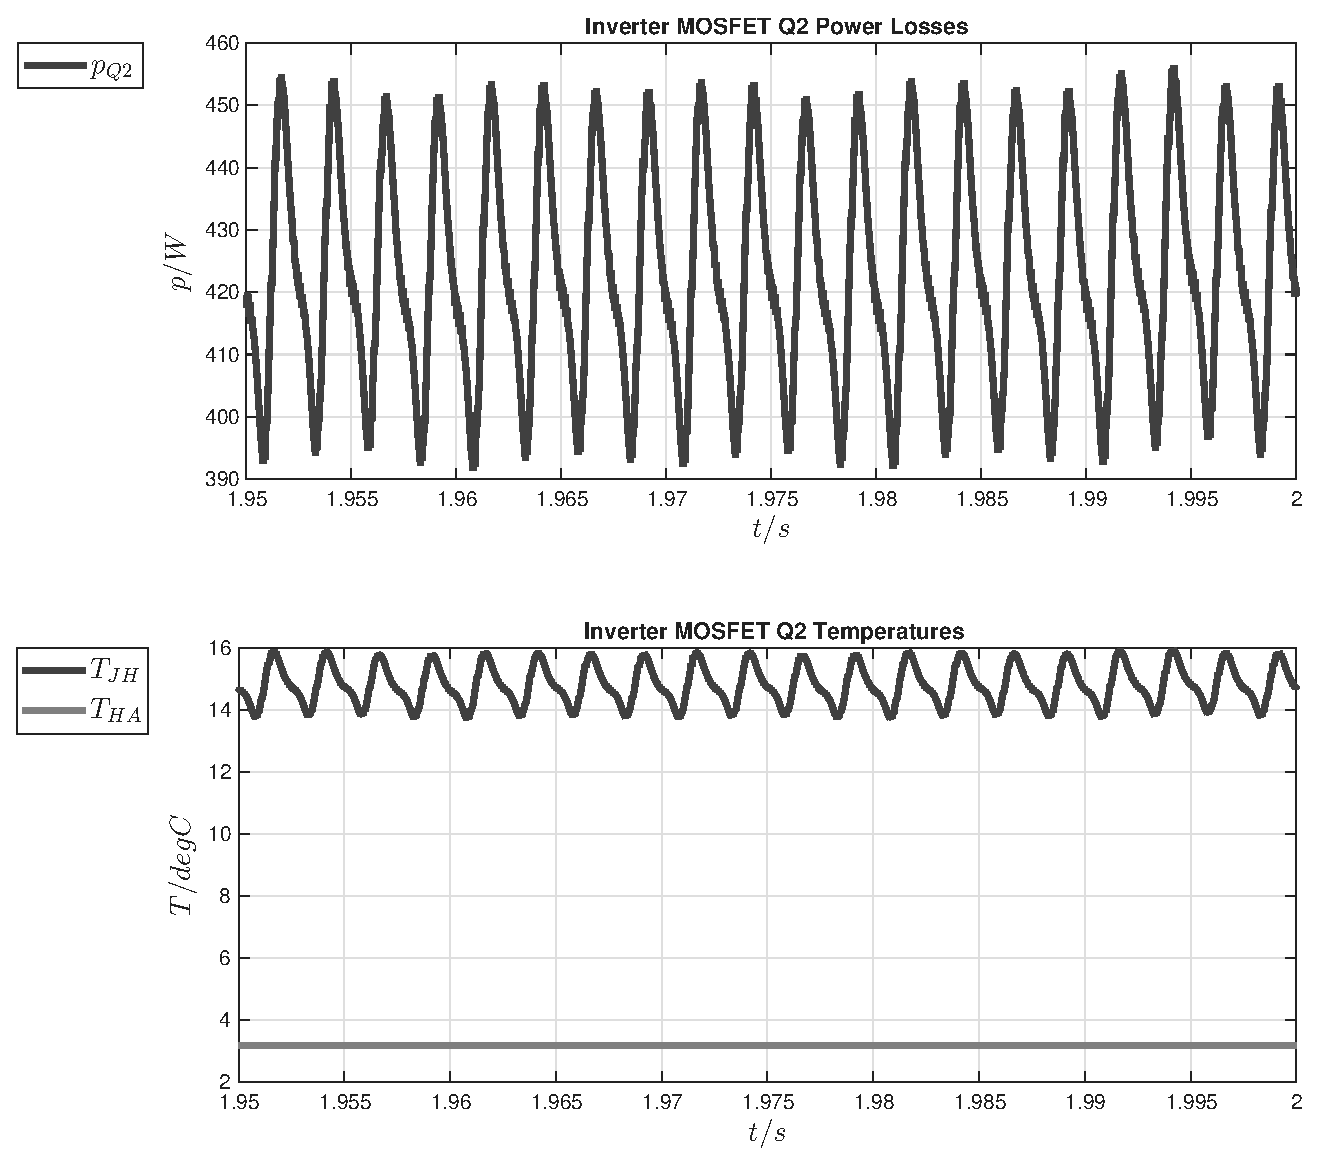
\includegraphics[width =225pt, angle = 0, 
		keepaspectratio]{figures/sim_results_400Hz_10kHz_1/inverter_Q2_power_losses.eps}
		\captionsetup{width=0.75\textwidth, font=footnotesize}	
		\caption{Inverter MOSFET Q2 power loss (top), and junction-case temperature (bottom).}
		\label{inverter_Q2_power_losses_400Hz}
	\end{subfigure}
	\captionsetup{width=0.65\textwidth, font=small}	
	\caption{Inverter MOSFETs thermal performance.}
	\label{}
\end{figure}

\begin{figure}[H]
	\centering
	\begin{subfigure}{0.5\textwidth}
		\centering
		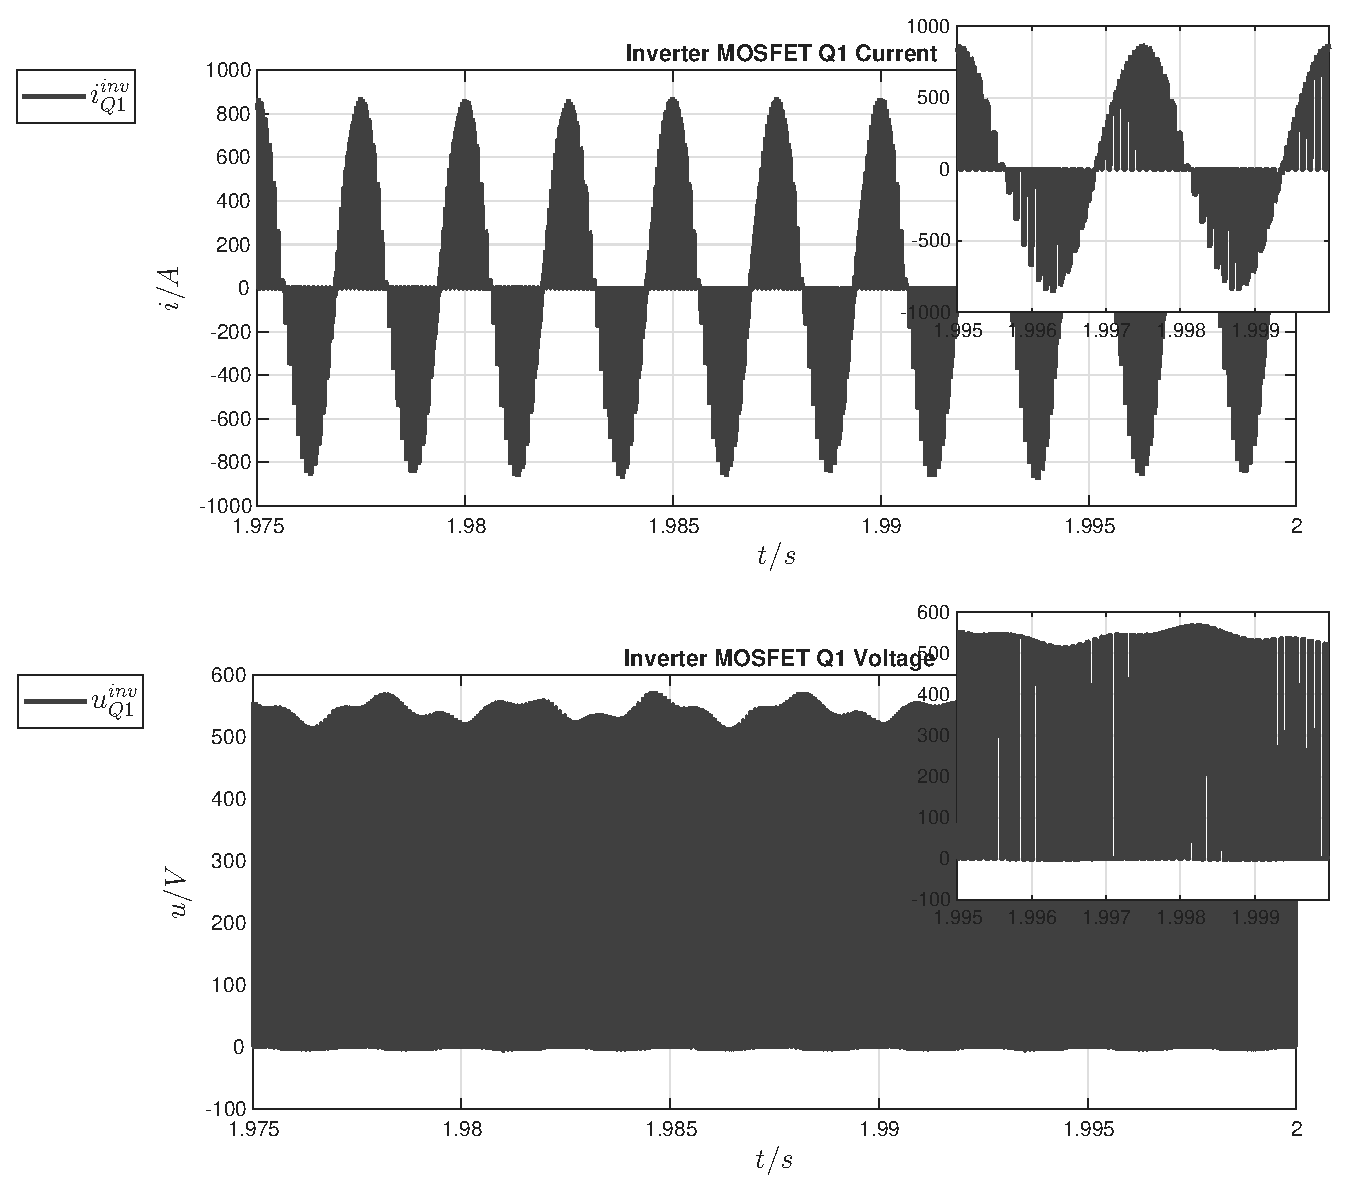
\includegraphics[width =225pt, angle = 0, 
		keepaspectratio]{figures/sim_results_400Hz_10kHz_1/inverter_mosfet_Q1_iu.eps}
		\captionsetup{width=0.65\textwidth, font=footnotesize}	
		\caption{Inverter MOSFET Q1 current (top), and voltage (bottom).}
		\label{inverter_mosfet_Q1_iu_400Hz}
	\end{subfigure}%
	\begin{subfigure}{0.5\textwidth}
		\centering
		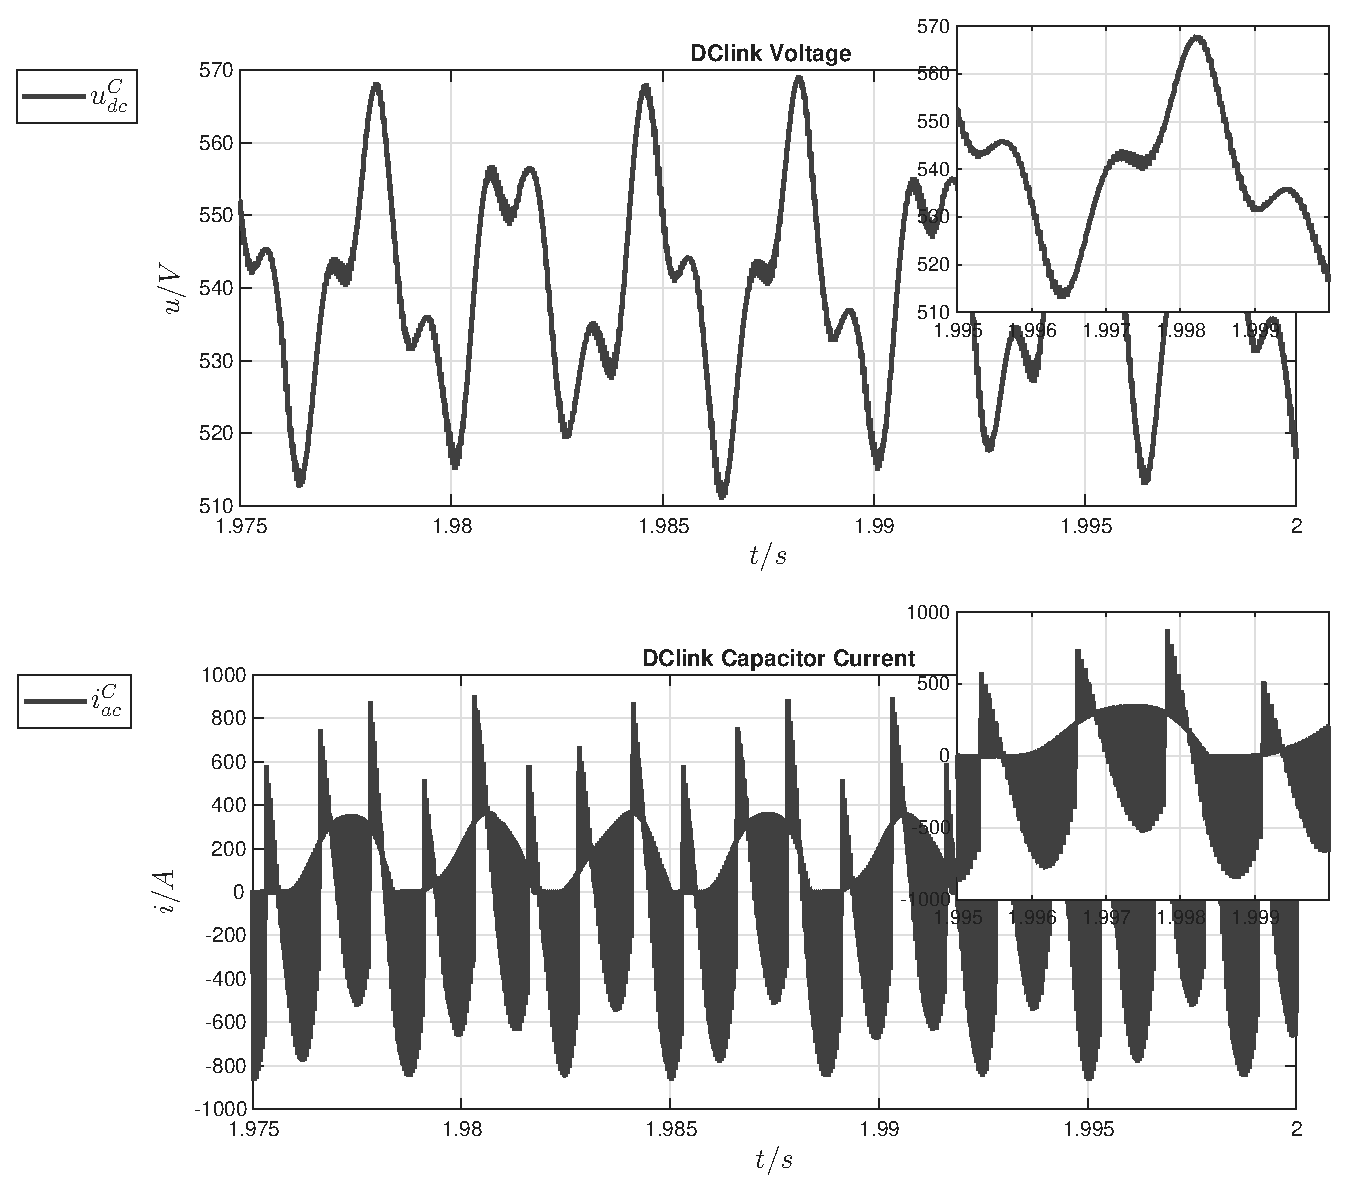
\includegraphics[width =225pt, angle = 0, 
		keepaspectratio]{figures/sim_results_400Hz_10kHz_1/dclink_ui.eps}
		\captionsetup{width=0.75\textwidth, font=footnotesize}	
		\caption{DClink voltage (top), and dclink capcitor current (bottom).}
		\label{dclink_ui_400Hz}
	\end{subfigure}
	\captionsetup{width=0.65\textwidth, font=small}	
	\caption{Inverter MOSFETs, and DClink quantities.}
	\label{}
\end{figure}

\begin{figure}[H]
	\centering
	\begin{subfigure}{0.5\textwidth}
		\centering
		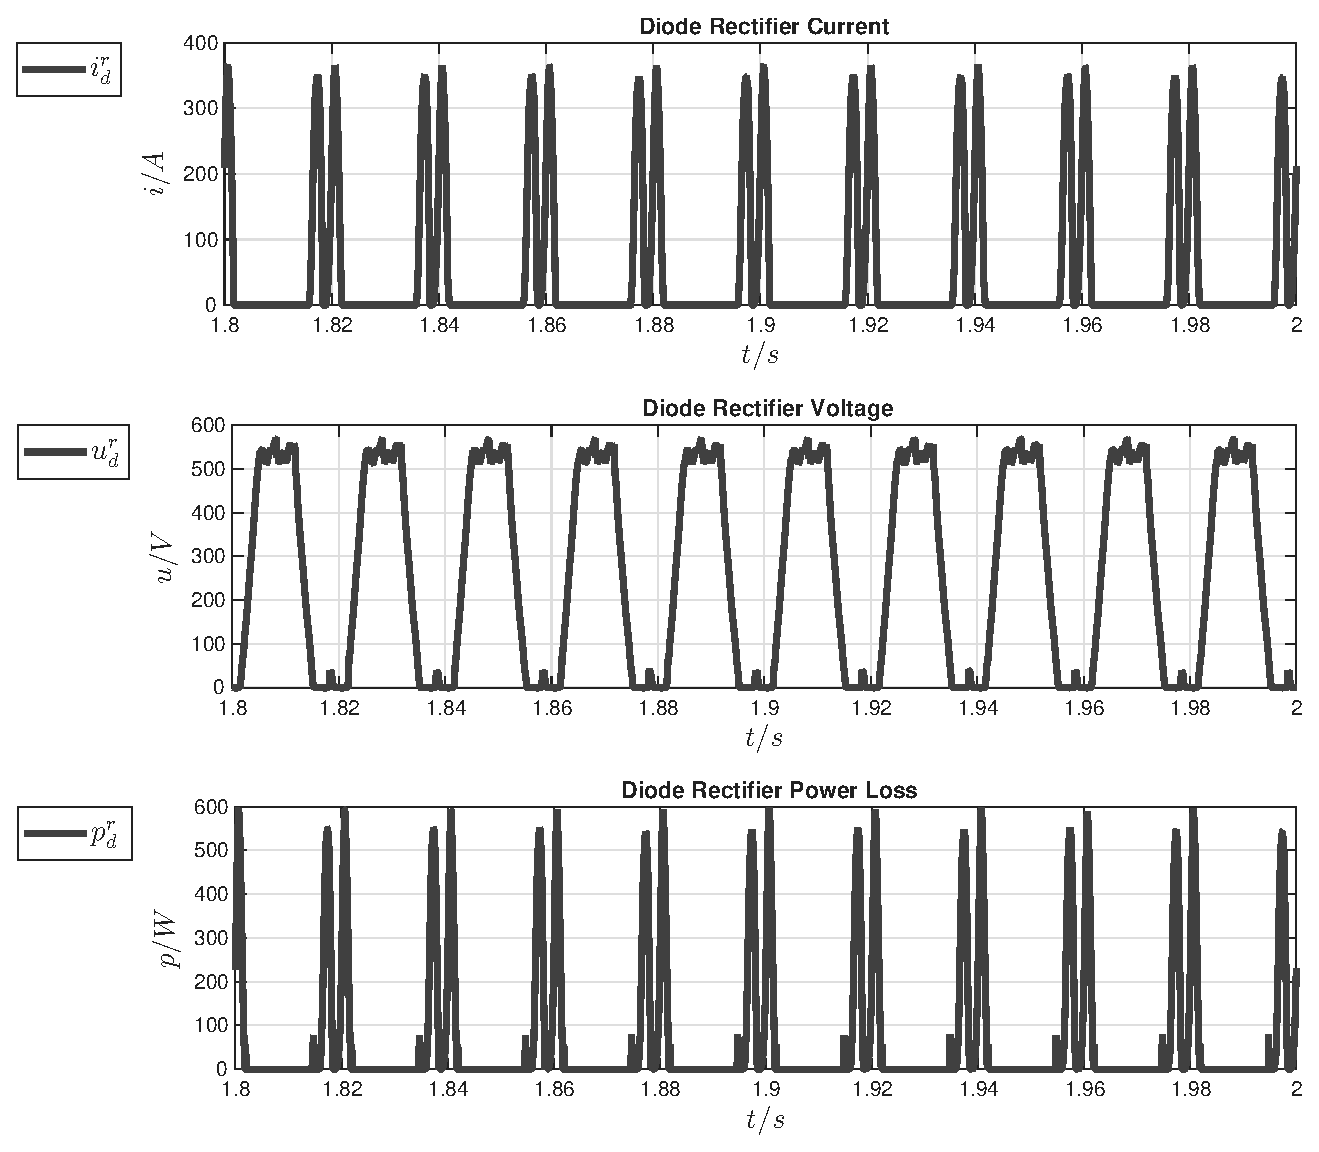
\includegraphics[width =225pt, angle = 0, 
		keepaspectratio]{figures/sim_results_400Hz_10kHz_1/diode_rectifier.eps}
		\captionsetup{width=0.65\textwidth, font=footnotesize}	
		\caption{Diode D1 rectifier current (top), voltage (center), and power loss (bottom).}
		\label{diode_rectifier_400Hz}
	\end{subfigure}%
	\begin{subfigure}{0.5\textwidth}
		\centering
		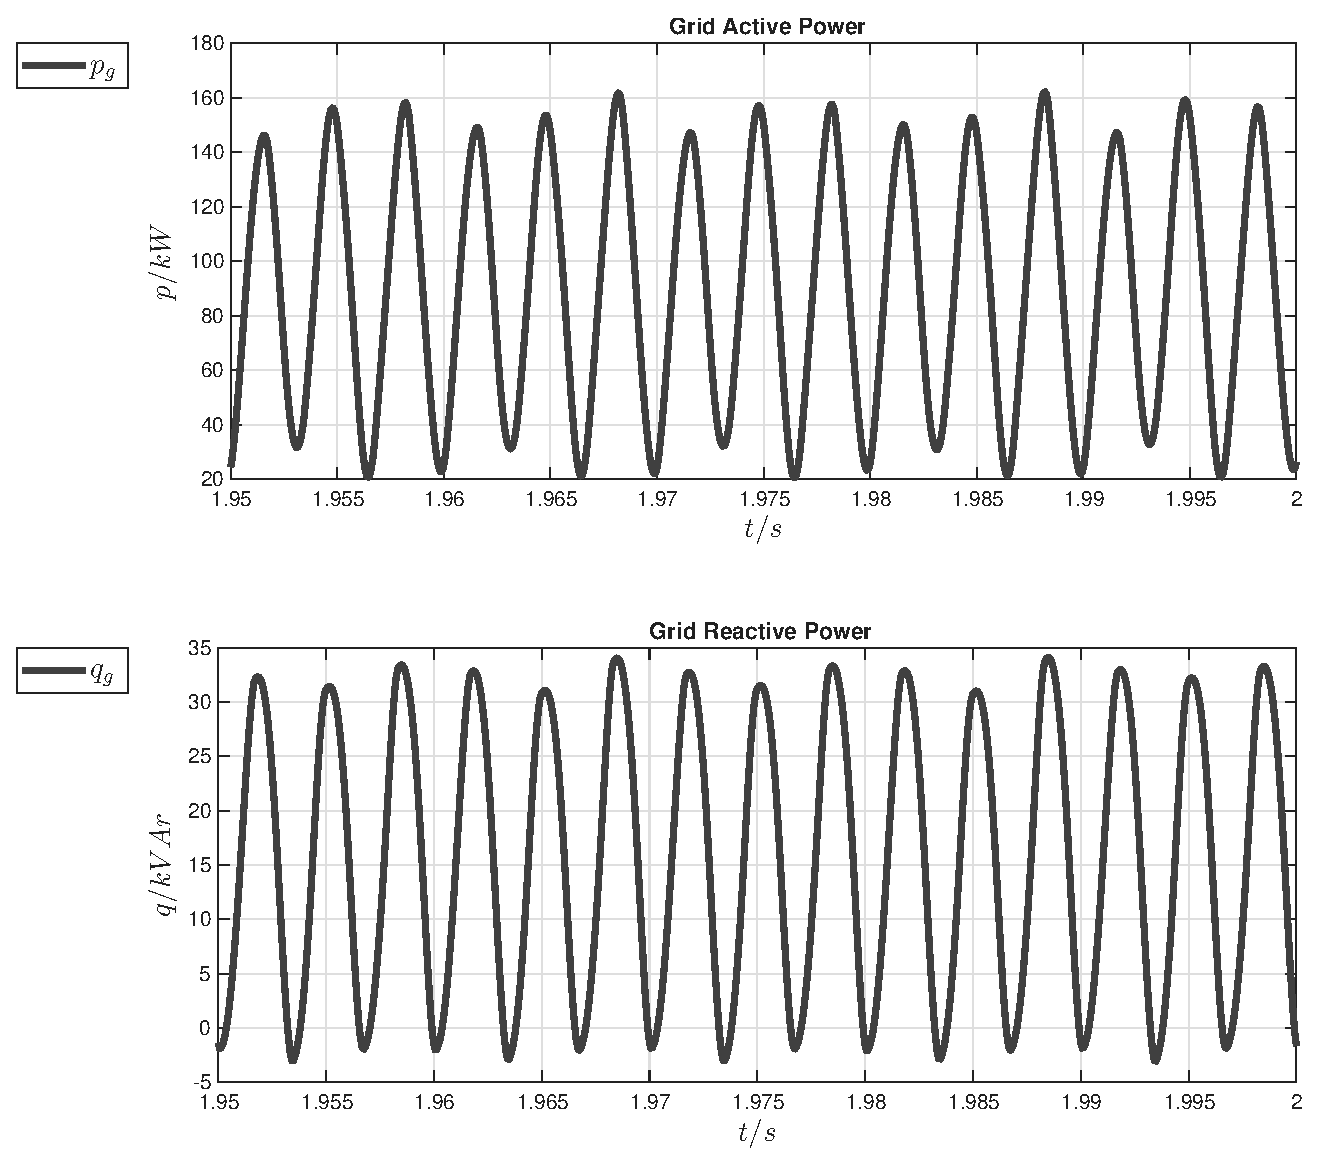
\includegraphics[width =225pt, angle = 0, 
		keepaspectratio]{figures/sim_results_400Hz_10kHz_1/grid_power.eps}
		\captionsetup{width=0.75\textwidth, font=footnotesize}	
		\caption{Grid active power (top), and grid reactive power (bottom) - measure implemented according to IEC.}
		\label{grid_power_400Hz}
	\end{subfigure}
	\captionsetup{width=0.65\textwidth, font=small}	
	\caption{Rectifier diode quantities and grid power analysis.}
	\label{}
\end{figure}

\begin{figure}[H]
	\centering
	\begin{subfigure}{0.5\textwidth}
		\centering
		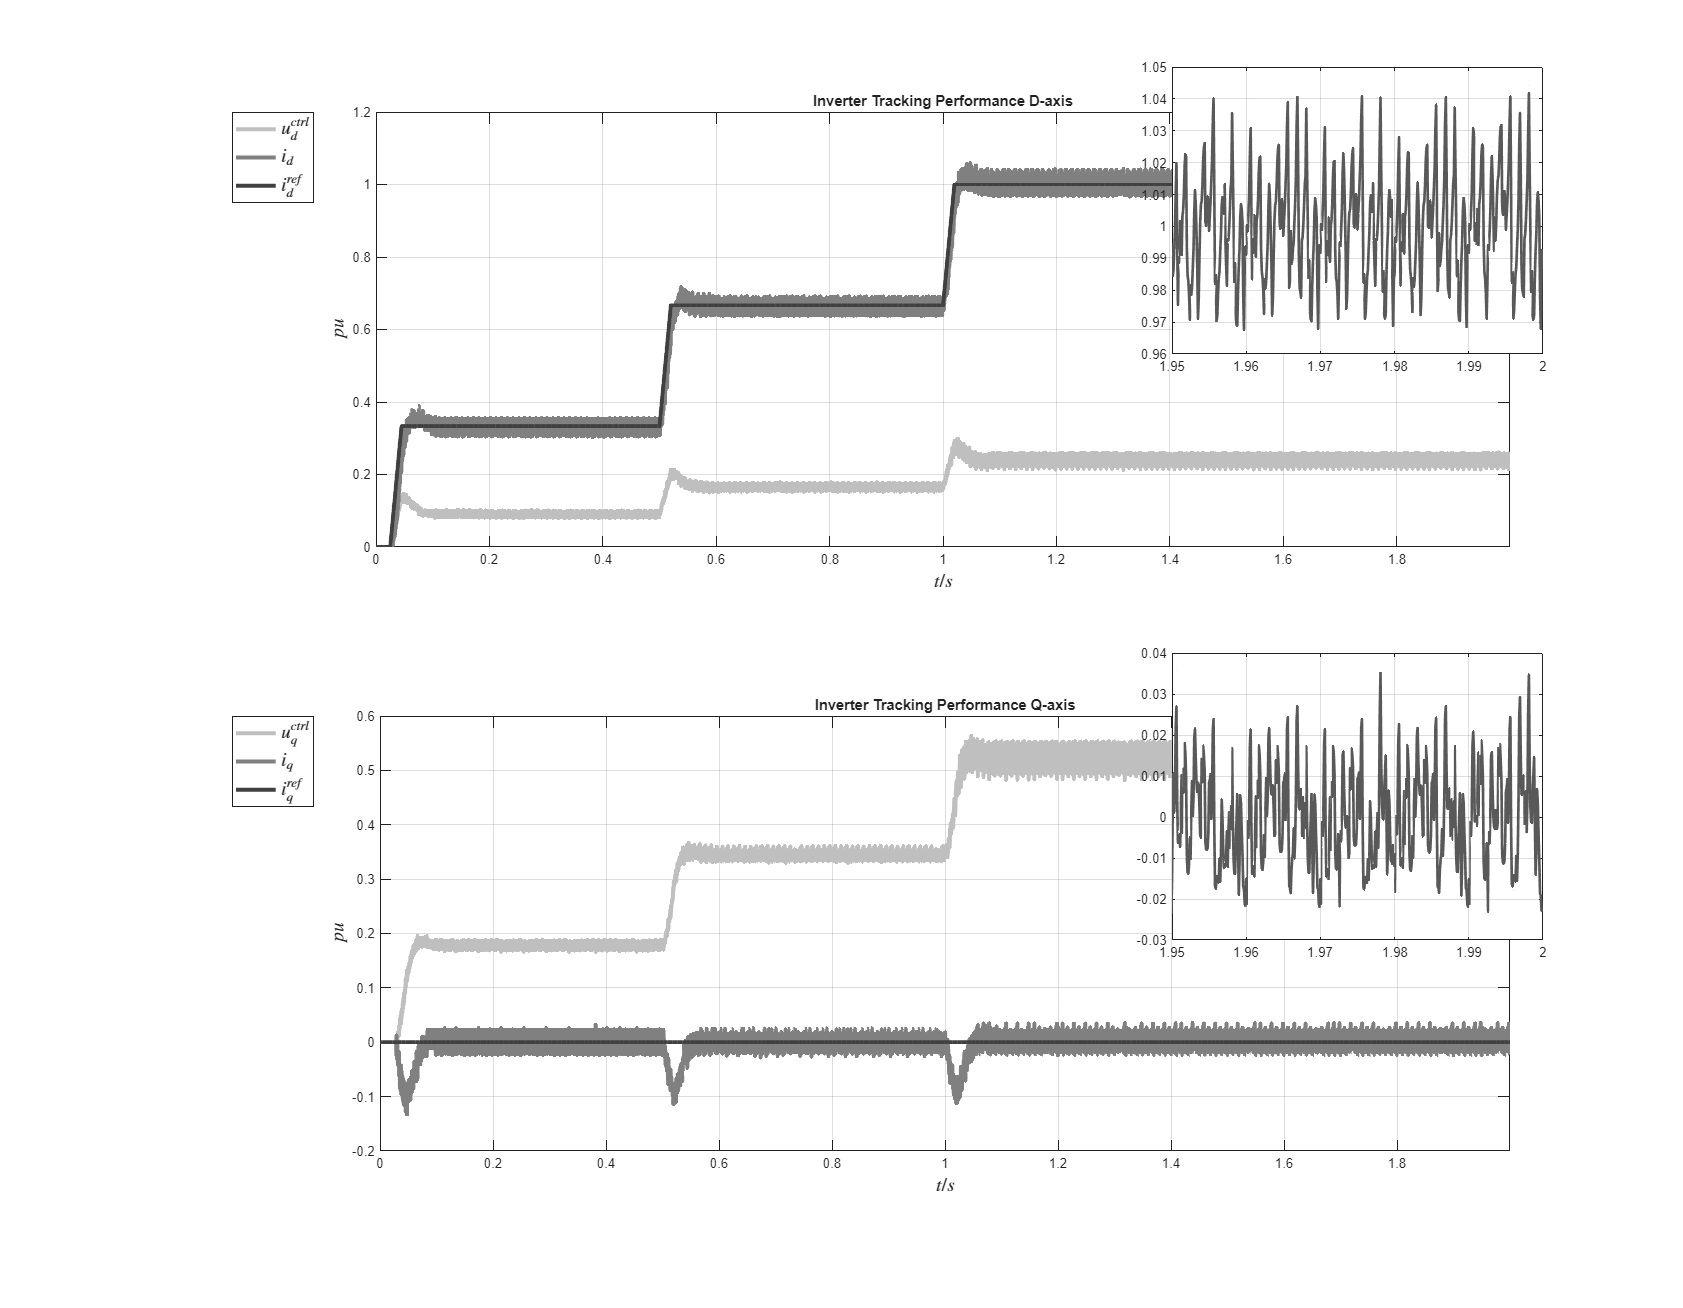
\includegraphics[width =265pt, angle = 0, 
		keepaspectratio]{figures/sim_results_400Hz_10kHz_1/inverter_current_control_1.eps}
		\captionsetup{width=0.65\textwidth, font=footnotesize}	
		\caption{Single phase tracking performance: along D-axis (top), along Q-axis (bottom).}
		\label{inverter_current_control_1_400Hz}
	\end{subfigure}%
	\begin{subfigure}{0.5\textwidth}
		\centering
		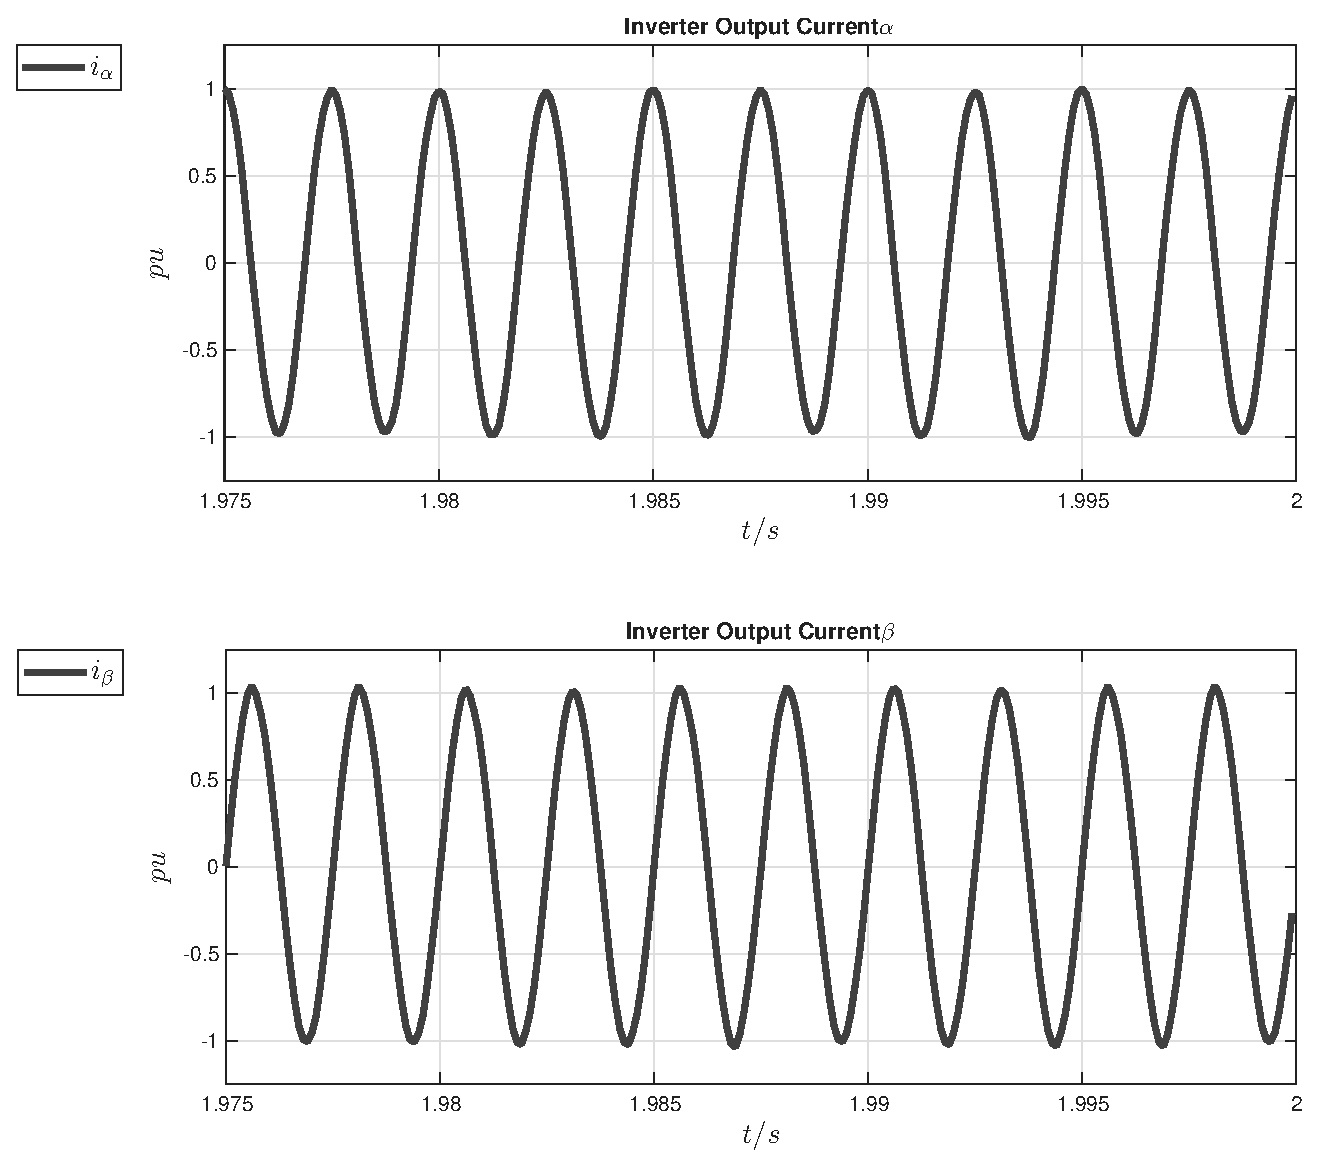
\includegraphics[width =225pt, angle = 0, 
		keepaspectratio]{figures/sim_results_400Hz_10kHz_1/inverter_current_control_2.eps}
		\captionsetup{width=0.75\textwidth, font=footnotesize}	
		\caption{Single phase output current (top), and equivalent shifted by the \textbf{phase-shift-filter} (bottom).}
		\label{inverter_current_control_2_400Hz}
	\end{subfigure}
	\captionsetup{width=0.65\textwidth, font=small}	
	\caption{Single phase inverter control performance.}
	\label{}
\end{figure}

\begin{figure}[H]
	\centering
	\begin{subfigure}{0.5\textwidth}
		\centering
		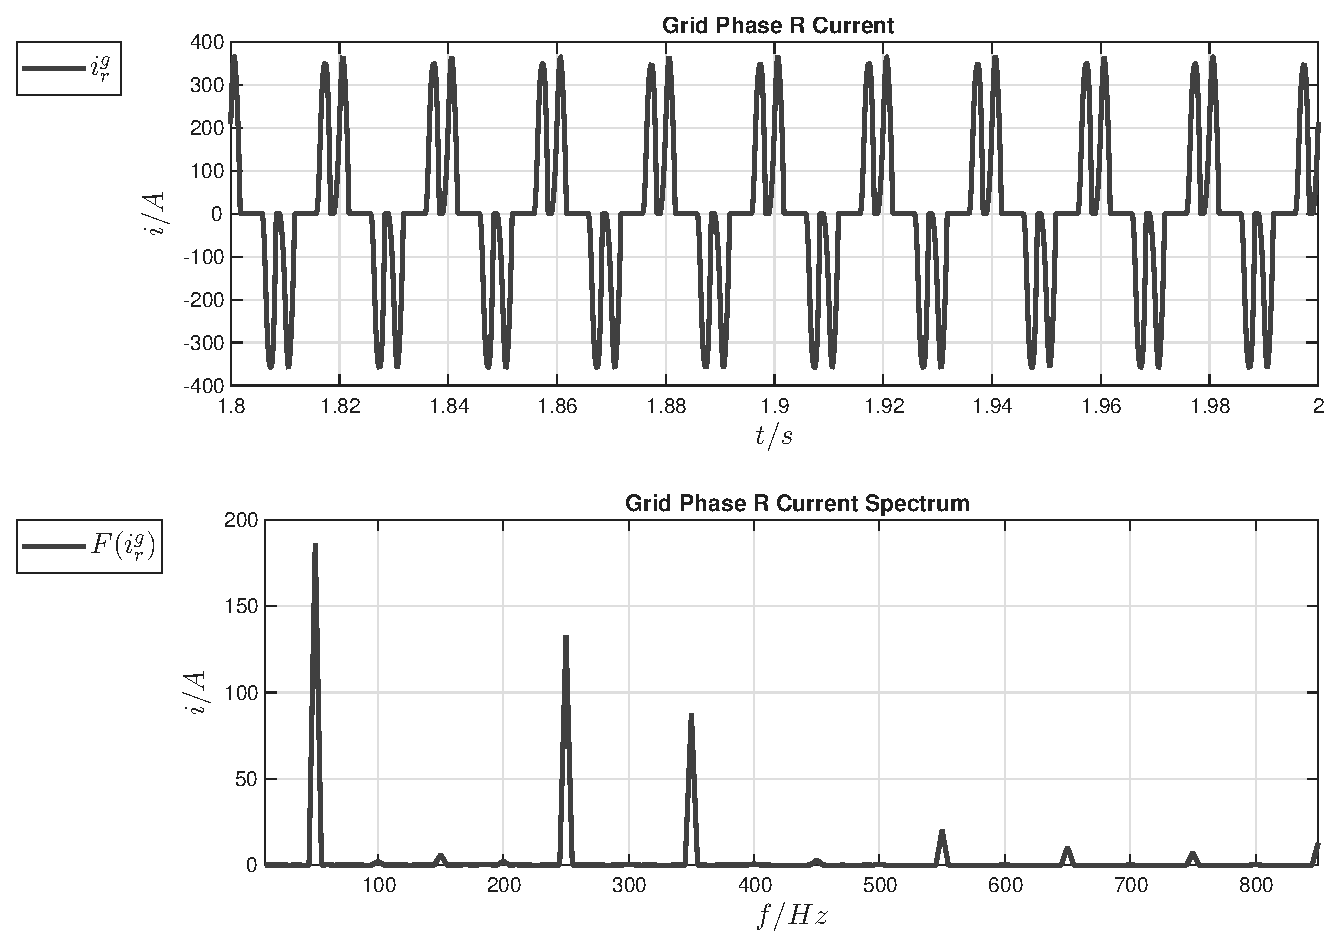
\includegraphics[width = 225pt, angle = 0, 
		keepaspectratio]{figures/sim_results_400Hz_10kHz_1/spectrum_grid_current_r.eps}
		\captionsetup{width=0.65\textwidth, font=footnotesize}	
		\caption{Grid phase current R (top), and grid phase current R spectrum (bottom).}
		\label{spectrum_grid_current_r_400Hz}
	\end{subfigure}%
	\begin{subfigure}{0.5\textwidth}
		\centering
		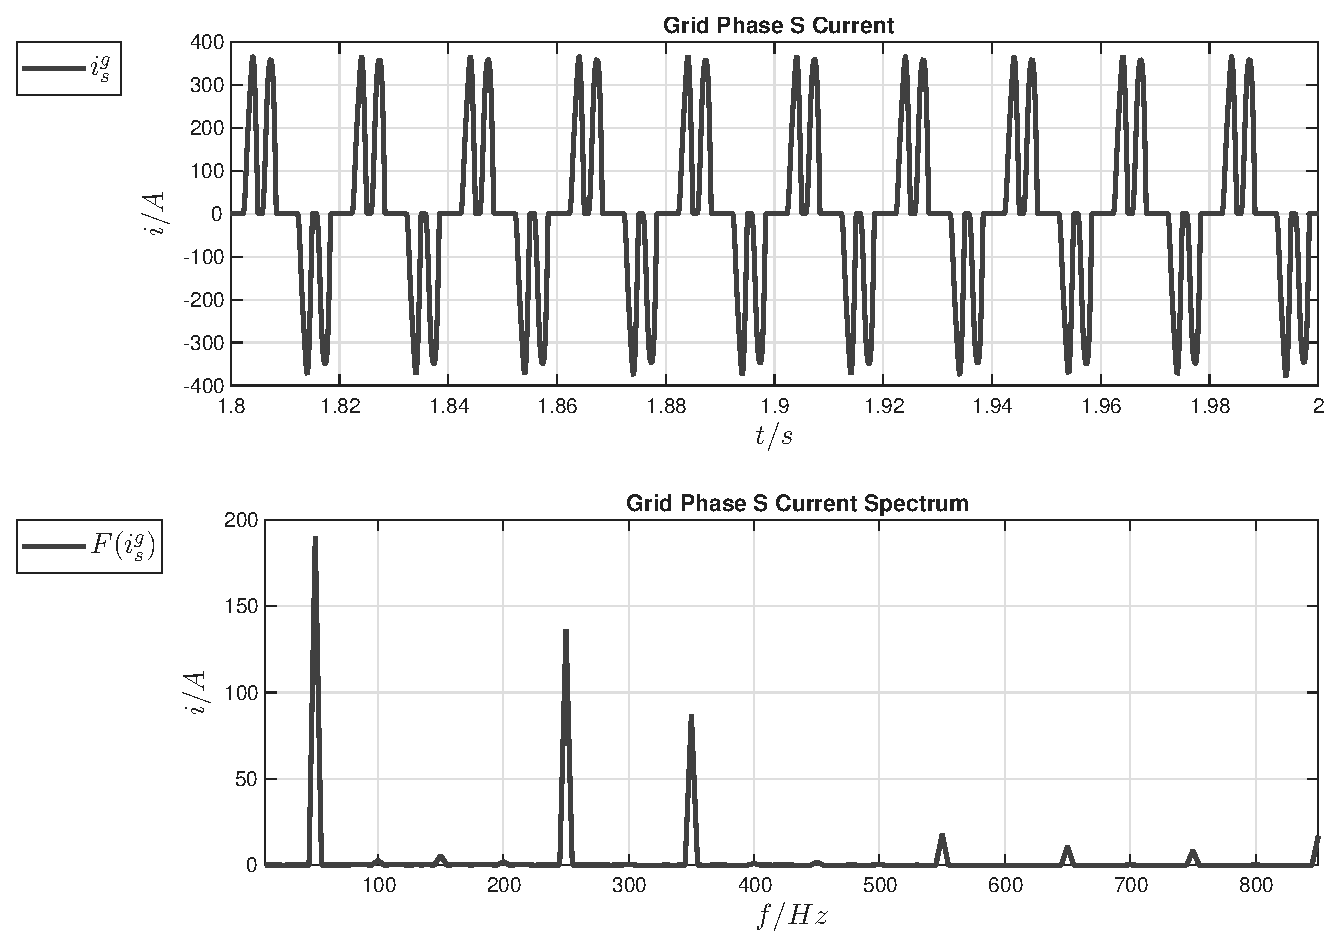
\includegraphics[width =225pt, angle = 0, 
		keepaspectratio]{figures/sim_results_400Hz_10kHz_1/spectrum_grid_current_s.eps}
		\captionsetup{width=0.75\textwidth, font=footnotesize}	
		\caption{Grid phase current S (top), and grid phase current S spectrum (bottom).}
		\label{spectrum_grid_current_s_400Hz}
	\end{subfigure}
	\captionsetup{width=0.65\textwidth, font=small}	
	\caption{Grid current harmonic analysis.}
	\label{}
\end{figure}



\begin{thebibliography}{99}
	% power electronics
	\bibitem{liserre} 
	R. Teodorescu, M. Liserre, P. Rodrıguez, \emph{Grid converters for photovoltaic and wind power systems}. Wiley, 2011.
\end{thebibliography}

\end{onehalfspace}
\end{document} 